% ******************************************************************************
% (c) NewTec GmbH 2019
%
% $URL: https://svn/nt/IMS/trunk/Entwicklung/Standard/Werkzeuge/mksource/system/Implementation/etc/c_c++/svn/h.tem $
% $Rev: 1377 $
% $Date: 2011-05-05 10:38:59 +0200 (Do, 05 Mai 2011) $
% $Author: $
% ******************************************************************************

% ******************************************************************************
% Definition einer Fusszeile fuer Ausgaben im HTML- und CHM-Format
%
% Diese Datei beinhaltet die Definition fuer die Fusszeile bei der
% Erstellung einer Detaillierten Software Design Dokumentation unter
% Verwendung von Doxygen.
% Folgende Dokumente koennen erzeugt werden:
% + PDF-Datei als Dokumentation zur Ansicht mit einem PDF-Reader
%
% Bitte unten in der entsprechenden Zeilen eintragen.
% Hinweis: Wird das Zeichen "_" verwendet, muss ein "\" davor gesetzt werden,
%          da es sonst als LaTeX-Kommando interpretiert wird.
% ******************************************************************************

\newcommand{\NTProjectname}{!!!Project Name2}
\newcommand{\NTDocumenttitle}{Detailed Software Design}
\newcommand{\NTVersion}{!!!0.12}
\newcommand{\NTDocumentnumber}{110012\_00992\_00882\_SWDD}
\newcommand{\NTCompanyNT}{NewTec GmbH
			\\Buchenweg 3
			\\89284 Pfaffenhofen a. d. Roth
			\\DEUTSCHLAND
}
\newcommand{\NTCompanyCustomer}{!!!Customer2
			\\!!!Customer department2
			\\!!!Customer Street 12
			\\!!!Customer location2
			\\!!!Germany2
}

% ******************************************************************************
% Ende mit manueller Bearbeitung.
% ******************************************************************************

% Latex header for doxygen 1.8.13
\documentclass[twoside]{book}

% Packages required by doxygen
\usepackage{fixltx2e}
\usepackage{calc}
\usepackage{doxygen}
\usepackage[export]{adjustbox} % also loads graphicx
\usepackage{graphicx}
\usepackage[utf8]{inputenc}
\usepackage{makeidx}
\usepackage{multicol}
\usepackage{multirow}
\PassOptionsToPackage{warn}{textcomp}
\usepackage{textcomp}
\usepackage[nointegrals]{wasysym}
\usepackage[table]{xcolor}

% Font selection
\usepackage[T1]{fontenc}
\usepackage[scaled=.90]{helvet}
\usepackage{courier}
\usepackage{amssymb}
\usepackage{sectsty}
\renewcommand{\familydefault}{\sfdefault}
\allsectionsfont{%
  \fontseries{bc}\selectfont%
  \color{darkgray}%
}
\renewcommand{\DoxyLabelFont}{%
  \fontseries{bc}\selectfont%
  \color{darkgray}%
}
\newcommand{\+}{\discretionary{\mbox{\scriptsize$\hookleftarrow$}}{}{}}

% Page & text layout
\usepackage{geometry}
\geometry{%
  a4paper,%
  top=2.5cm,%
  bottom=2.5cm,%
  left=2.5cm,%
  right=2.5cm%
}
\tolerance=750
\hfuzz=15pt
\hbadness=750
\setlength{\emergencystretch}{15pt}
\setlength{\parindent}{0cm}
\setlength{\parskip}{3ex plus 2ex minus 2ex}
\makeatletter
\renewcommand{\paragraph}{%
  \@startsection{paragraph}{4}{0ex}{-1.0ex}{1.0ex}{%
    \normalfont\normalsize\bfseries\SS@parafont%
  }%
}
\renewcommand{\subparagraph}{%
  \@startsection{subparagraph}{5}{0ex}{-1.0ex}{1.0ex}{%
    \normalfont\normalsize\bfseries\SS@subparafont%
  }%
}
\makeatother

% Headers & footers
\usepackage{fancyhdr}
\pagestyle{fancyplain}
\fancyhead[LE]{\fancyplain{}{\NTProjectname \\ \NTDocumenttitle}}
\fancyhead[CE]{\fancyplain{}{}}
\fancyhead[RE]{\fancyplain{}{
\includegraphics[scale=0.2]{110012_00992_00882_IMG-NewTecLogoSmall.jpg}}}
\fancyhead[LO]{\fancyplain{}{
\includegraphics[scale=0.2]{110012_00992_00882_IMG-NewTecLogoSmall.jpg}}}
\fancyhead[CO]{\fancyplain{}{}}
\fancyhead[RO]{\fancyplain{}{\NTProjectname \\ \NTDocumenttitle}}
\fancyfoot[LE]{\fancyplain{}{\bfseries\scriptsize Doc.-No.:\\ \NTDocumentnumber}}
\fancyfoot[CE]{\fancyplain{}{\bfseries\scriptsize Version: \NTVersion \\Issue Date: Tue Jan 30 2024 11:29:40}}
\fancyfoot[RE]{\fancyplain{}{\bfseries \scriptsize Page \thepage \ of \pageref{LastPage} \tiny \\ \  \\ Generated by Doxygen 1.8.7}}
\fancyfoot[LO]{\fancyplain{}{\bfseries \scriptsize Page \thepage \ of \pageref{LastPage} \tiny \\ \  \\ Generated by Doxygen 1.8.7}}
\fancyfoot[CO]{\fancyplain{}{\bfseries\scriptsize Version: \NTVersion \\Issue Date: Tue Jan 30 2024 11:29:40}}
\fancyfoot[RO]{\fancyplain{}{\bfseries\scriptsize Doc.-No.:\\ \NTDocumentnumber}}
\renewcommand{\footrulewidth}{0.4pt}
\renewcommand{\chaptermark}[1]{%
  \markboth{#1}{}%
}
\renewcommand{\sectionmark}[1]{%
  \markright{\thesection\ #1}%
}

% Indices & bibliography
\usepackage{natbib}
\usepackage[titles]{tocloft}
\setcounter{tocdepth}{3}
\setcounter{secnumdepth}{5}
\makeindex

% Hyperlinks (required, but should be loaded last)
\usepackage{ifpdf}
\ifpdf
  \usepackage[pdftex,pagebackref=true]{hyperref}
\else
  \usepackage[ps2pdf,pagebackref=true]{hyperref}
\fi
\hypersetup{%
  colorlinks=true,%
  linkcolor=blue,%
  citecolor=blue,%
  unicode%
}

% Background image at the title page
\usepackage[firstpage=true]{background}
\backgroundsetup{
    position=current page.south,
    angle=0,
    nodeanchor=south west,
    vshift=-5mm,
    opacity=0.6,
    scale=1,
    contents={%
        
\includegraphics[scale=0.6]{110012_00992_00882_IMG-NewTecBallGrid.png}
    }%
}

% Custom commands
\newcommand{\clearemptydoublepage}{%
  \newpage{\pagestyle{empty}\cleardoublepage}%
}

\usepackage{caption}
\captionsetup{labelsep=space,justification=centering,font={bf},singlelinecheck=off,skip=4pt,position=top}

% NT blue color
\definecolor{ntblue}{RGB}{0, 118, 189}

%===== C O N T E N T S =====

\begin{document}

% Titlepage & ToC
\hypersetup{pageanchor=false,
             bookmarks=true,
             bookmarksnumbered=true,
             pdfencoding=unicode
            }
\pagenumbering{arabic}
\begin{titlepage}
{\hfill 
\includegraphics[scale=0.2]{110012_00992_00882_IMG-NewTecSloganLogo.jpg}}\\
\vspace*{4cm}\\
{\Large \textcolor{ntblue}{\_\_\_\_}}\\
\\
{\huge \textcolor{ntblue}{\textit{\NTDocumenttitle}}}\\
{\Large \textcolor{ntblue}{\textit{\NTProjectname}}}\\
{\Large \textcolor{ntblue}{\_\_\_\_}}\\
\vspace*{1.5cm}\\
{\small Doc.-No.:\quad\NTDocumentnumber}\\
{\small Doc.-Version.:\quad\NTVersion}\\
\vspace*{5cm}\\
Customer:\\
\NTCompanyCustomer\\
\vspace*{1.5cm}\\
Author:\\
\NTCompanyNT
\end{titlepage}
\clearemptydoublepage
\tableofcontents
\clearemptydoublepage
\hypersetup{pageanchor=true}

%--- Begin generated contents ---
\chapter{Main Page}
\label{index}\hypertarget{index}{}Version\+: !!!0.12

\subsection*{Customer}

!!!\+Customer2~\newline
!!!\+Customer department2~\newline
!!!\+Customer Street 12~\newline
!!!\+Customer location2~\newline
!!!\+Germany2

\subsection*{Author}

New\+Tec Gmb\+H~\newline
Buchenweg 3~\newline
89284 Pfaffenhofen a. d. Roth~\newline
D\+E\+U\+T\+S\+C\+H\+L\+A\+N\+D 
\chapter{Module Index}
\section{Modules}
Here is a list of all modules\+:\begin{DoxyCompactList}
\item \contentsline{section}{App}{\pageref{group___app}}{}
\item \contentsline{section}{Global}{\pageref{group___global__group}}{}
\item \contentsline{section}{Os}{\pageref{group___os}}{}
\end{DoxyCompactList}

\chapter{Data Structure Index}
\section{Data Structures}
Here are the data structures with brief descriptions\+:\begin{DoxyCompactList}
\item\contentsline{section}{\hyperlink{structtag___soft_timer}{tag\+\_\+\+Soft\+Timer} \\*Soft\+Timer data structure }{\pageref{structtag___soft_timer}}{}
\item\contentsline{section}{\hyperlink{structtag___task}{tag\+\_\+\+Task} \\*Task Structure }{\pageref{structtag___task}}{}
\end{DoxyCompactList}

\chapter{File Index}
\section{File List}
Here is a list of all documented files with brief descriptions\+:\begin{DoxyCompactList}
\item\contentsline{section}{src/app/\hyperlink{_main_task_8c}{Main\+Task.\+c} \\*Main Application task }{\pageref{_main_task_8c}}{}
\item\contentsline{section}{src/app/\hyperlink{_main_task_8h}{Main\+Task.\+h} \\*The main application task }{\pageref{_main_task_8h}}{}
\item\contentsline{section}{src/\+Common/\hyperlink{_types_8h}{Types.\+h} \\*Basic types definition for A\+Tmega128 }{\pageref{_types_8h}}{}
\item\contentsline{section}{src/os/\hyperlink{_error_handler_8c}{Error\+Handler.\+c} \\*Error\+Handler for all error processing }{\pageref{_error_handler_8c}}{}
\item\contentsline{section}{src/os/\hyperlink{_error_handler_8h}{Error\+Handler.\+h} \\*Enter short description here }{\pageref{_error_handler_8h}}{}
\item\contentsline{section}{src/os/\hyperlink{_os_8c}{Os.\+c} \\*O\+S main module }{\pageref{_os_8c}}{}
\item\contentsline{section}{src/os/\hyperlink{_os_8h}{Os.\+h} \\*Main header for O\+S module }{\pageref{_os_8h}}{}
\item\contentsline{section}{src/os/\hyperlink{_scheduler_8c}{Scheduler.\+c} \\*Simple task scheduler }{\pageref{_scheduler_8c}}{}
\item\contentsline{section}{src/os/\hyperlink{_scheduler_8h}{Scheduler.\+h} \\*Cooperative Round-\/\+Robin Scheduler }{\pageref{_scheduler_8h}}{}
\item\contentsline{section}{src/os/\hyperlink{_soft_timer_8c}{Soft\+Timer.\+c} \\*Soft\+Timer implementation }{\pageref{_soft_timer_8c}}{}
\item\contentsline{section}{src/os/\hyperlink{_soft_timer_8h}{Soft\+Timer.\+h} \\*Soft\+Timer definiton }{\pageref{_soft_timer_8h}}{}
\item\contentsline{section}{src/os/\hyperlink{_task_8c}{Task.\+c} \\*Simple task scheduler }{\pageref{_task_8c}}{}
\item\contentsline{section}{src/os/\hyperlink{_task_8h}{Task.\+h} \\*Enter short description here }{\pageref{_task_8h}}{}
\end{DoxyCompactList}

\chapter{Module Documentation}
\hypertarget{group___app}{\section{App}
\label{group___app}\index{App@{App}}
}
\subsection*{Files}
\begin{DoxyCompactItemize}
\item 
file \hyperlink{_main_task_8c}{Main\+Task.\+c}
\begin{DoxyCompactList}\small\item\em Main Application task. \end{DoxyCompactList}\item 
file \hyperlink{_main_task_8h}{Main\+Task.\+h}
\begin{DoxyCompactList}\small\item\em The main application task. \end{DoxyCompactList}\end{DoxyCompactItemize}


\subsection{Detailed Description}

\hypertarget{group___global__group}{\section{Global}
\label{group___global__group}\index{Global@{Global}}
}
\subsection*{Files}
\begin{DoxyCompactItemize}
\item 
file \hyperlink{_types_8h}{Types.\+h}
\begin{DoxyCompactList}\small\item\em Basic types definition for A\+Tmega128. \end{DoxyCompactList}\end{DoxyCompactItemize}


\subsection{Detailed Description}

\hypertarget{group___os}{\section{Os}
\label{group___os}\index{Os@{Os}}
}
\subsection*{Files}
\begin{DoxyCompactItemize}
\item 
file \hyperlink{_error_handler_8c}{Error\+Handler.\+c}
\begin{DoxyCompactList}\small\item\em Error\+Handler for all error processing. \end{DoxyCompactList}\item 
file \hyperlink{_error_handler_8h}{Error\+Handler.\+h}
\begin{DoxyCompactList}\small\item\em Enter short description here. \end{DoxyCompactList}\item 
file \hyperlink{_os_8c}{Os.\+c}
\begin{DoxyCompactList}\small\item\em O\+S main module. \end{DoxyCompactList}\item 
file \hyperlink{_os_8h}{Os.\+h}
\begin{DoxyCompactList}\small\item\em Main header for O\+S module. \end{DoxyCompactList}\item 
file \hyperlink{_scheduler_8c}{Scheduler.\+c}
\begin{DoxyCompactList}\small\item\em Simple task scheduler. \end{DoxyCompactList}\item 
file \hyperlink{_scheduler_8h}{Scheduler.\+h}
\begin{DoxyCompactList}\small\item\em Cooperative Round-\/\+Robin Scheduler. \end{DoxyCompactList}\item 
file \hyperlink{_soft_timer_8c}{Soft\+Timer.\+c}
\begin{DoxyCompactList}\small\item\em Soft\+Timer implementation. \end{DoxyCompactList}\item 
file \hyperlink{_soft_timer_8h}{Soft\+Timer.\+h}
\begin{DoxyCompactList}\small\item\em Soft\+Timer definiton. \end{DoxyCompactList}\item 
file \hyperlink{_task_8c}{Task.\+c}
\begin{DoxyCompactList}\small\item\em Simple task scheduler. \end{DoxyCompactList}\item 
file \hyperlink{_task_8h}{Task.\+h}
\begin{DoxyCompactList}\small\item\em Enter short description here. \end{DoxyCompactList}\end{DoxyCompactItemize}


\subsection{Detailed Description}

\chapter{Data Structure Documentation}
\hypertarget{structtag___soft_timer}{\section{tag\+\_\+\+Soft\+Timer Struct Reference}
\label{structtag___soft_timer}\index{tag\+\_\+\+Soft\+Timer@{tag\+\_\+\+Soft\+Timer}}
}


Soft\+Timer data structure.  




{\ttfamily \#include $<$Soft\+Timer.\+h$>$}

\subsection*{Data Fields}
\begin{DoxyCompactItemize}
\item 
\hyperlink{_soft_timer_8h_a7f078e1503ae2d931bfbc6ada2145fed}{Soft\+Timer\+State} \hyperlink{structtag___soft_timer_af62379b52047ab99128f9a4b62905bc2}{state}
\begin{DoxyCompactList}\small\item\em Soft\+Timer state. \end{DoxyCompactList}\item 
volatile \hyperlink{_types_8h_aad0fc9943ec46ed9388d30c8ebe52b77}{U\+Int16} \hyperlink{structtag___soft_timer_ad35ffa049959bc406243952e7f3e738f}{counter}
\begin{DoxyCompactList}\small\item\em The countdown counter. \end{DoxyCompactList}\item 
\hyperlink{_types_8h_aad0fc9943ec46ed9388d30c8ebe52b77}{U\+Int16} \hyperlink{structtag___soft_timer_aa7b3fcf408e6ac60c9fc94ce0f202285}{thresh\+Hold}
\begin{DoxyCompactList}\small\item\em The countdown start value. \end{DoxyCompactList}\end{DoxyCompactItemize}


\subsection{Detailed Description}
Soft\+Timer data structure. 

\subsection{Field Documentation}
\hypertarget{structtag___soft_timer_ad35ffa049959bc406243952e7f3e738f}{\index{tag\+\_\+\+Soft\+Timer@{tag\+\_\+\+Soft\+Timer}!counter@{counter}}
\index{counter@{counter}!tag\+\_\+\+Soft\+Timer@{tag\+\_\+\+Soft\+Timer}}
\subsubsection[{counter}]{\setlength{\rightskip}{0pt plus 5cm}volatile {\bf U\+Int16} tag\+\_\+\+Soft\+Timer\+::counter}}\label{structtag___soft_timer_ad35ffa049959bc406243952e7f3e738f}


The countdown counter. 



Referenced by Soft\+Timer\+\_\+get(), Soft\+Timer\+\_\+init(), Soft\+Timer\+\_\+start(), Soft\+Timer\+\_\+\+Update(), and Soft\+Timer\+Handler\+\_\+update().

\hypertarget{structtag___soft_timer_af62379b52047ab99128f9a4b62905bc2}{\index{tag\+\_\+\+Soft\+Timer@{tag\+\_\+\+Soft\+Timer}!state@{state}}
\index{state@{state}!tag\+\_\+\+Soft\+Timer@{tag\+\_\+\+Soft\+Timer}}
\subsubsection[{state}]{\setlength{\rightskip}{0pt plus 5cm}{\bf Soft\+Timer\+State} tag\+\_\+\+Soft\+Timer\+::state}}\label{structtag___soft_timer_af62379b52047ab99128f9a4b62905bc2}


Soft\+Timer state. 



Referenced by Soft\+Timer\+\_\+init(), Soft\+Timer\+\_\+start(), Soft\+Timer\+\_\+\+Stop(), Soft\+Timer\+\_\+\+Update(), Soft\+Timer\+Handler\+\_\+register(), and Soft\+Timer\+Handler\+\_\+update().

\hypertarget{structtag___soft_timer_aa7b3fcf408e6ac60c9fc94ce0f202285}{\index{tag\+\_\+\+Soft\+Timer@{tag\+\_\+\+Soft\+Timer}!thresh\+Hold@{thresh\+Hold}}
\index{thresh\+Hold@{thresh\+Hold}!tag\+\_\+\+Soft\+Timer@{tag\+\_\+\+Soft\+Timer}}
\subsubsection[{thresh\+Hold}]{\setlength{\rightskip}{0pt plus 5cm}{\bf U\+Int16} tag\+\_\+\+Soft\+Timer\+::thresh\+Hold}}\label{structtag___soft_timer_aa7b3fcf408e6ac60c9fc94ce0f202285}


The countdown start value. 



Referenced by Soft\+Timer\+\_\+init(), Soft\+Timer\+\_\+restart(), and Soft\+Timer\+\_\+start().



The documentation for this struct was generated from the following file\+:\begin{DoxyCompactItemize}
\item 
src/os/\hyperlink{_soft_timer_8h}{Soft\+Timer.\+h}\end{DoxyCompactItemize}

\hypertarget{structtag___task}{\section{tag\+\_\+\+Task Struct Reference}
\label{structtag___task}\index{tag\+\_\+\+Task@{tag\+\_\+\+Task}}
}


Task Structure.  




{\ttfamily \#include $<$Task.\+h$>$}

\subsection*{Data Fields}
\begin{DoxyCompactItemize}
\item 
\hyperlink{_task_8h_a72a5e74cf680503ec09223c3cfdbf4e3}{Task\+State} \hyperlink{structtag___task_a9c1ed76fb17998c5d0eaea9476aca301}{state}
\begin{DoxyCompactList}\small\item\em Task status. \end{DoxyCompactList}\item 
void $\ast$ \hyperlink{structtag___task_a02bd6ed13271438c11b932a061b59f0c}{instance\+Data}
\begin{DoxyCompactList}\small\item\em Task context, passed to work function. \end{DoxyCompactList}\item 
\hyperlink{_task_8h_a8f3c61c0430299673ab83bf936073184}{Task\+Work\+Callback} \hyperlink{structtag___task_ad633bdb373da2f8a144e8a7927cb3630}{work\+Callback}
\begin{DoxyCompactList}\small\item\em Task work cycle function. \end{DoxyCompactList}\end{DoxyCompactItemize}


\subsection{Detailed Description}
Task Structure. 

\subsection{Field Documentation}
\hypertarget{structtag___task_a02bd6ed13271438c11b932a061b59f0c}{\index{tag\+\_\+\+Task@{tag\+\_\+\+Task}!instance\+Data@{instance\+Data}}
\index{instance\+Data@{instance\+Data}!tag\+\_\+\+Task@{tag\+\_\+\+Task}}
\subsubsection[{instance\+Data}]{\setlength{\rightskip}{0pt plus 5cm}void$\ast$ tag\+\_\+\+Task\+::instance\+Data}}\label{structtag___task_a02bd6ed13271438c11b932a061b59f0c}


Task context, passed to work function. 



Referenced by Task\+\_\+init().

\hypertarget{structtag___task_a9c1ed76fb17998c5d0eaea9476aca301}{\index{tag\+\_\+\+Task@{tag\+\_\+\+Task}!state@{state}}
\index{state@{state}!tag\+\_\+\+Task@{tag\+\_\+\+Task}}
\subsubsection[{state}]{\setlength{\rightskip}{0pt plus 5cm}{\bf Task\+State} tag\+\_\+\+Task\+::state}}\label{structtag___task_a9c1ed76fb17998c5d0eaea9476aca301}


Task status. 



Referenced by Task\+\_\+init().

\hypertarget{structtag___task_ad633bdb373da2f8a144e8a7927cb3630}{\index{tag\+\_\+\+Task@{tag\+\_\+\+Task}!work\+Callback@{work\+Callback}}
\index{work\+Callback@{work\+Callback}!tag\+\_\+\+Task@{tag\+\_\+\+Task}}
\subsubsection[{work\+Callback}]{\setlength{\rightskip}{0pt plus 5cm}{\bf Task\+Work\+Callback} tag\+\_\+\+Task\+::work\+Callback}}\label{structtag___task_ad633bdb373da2f8a144e8a7927cb3630}


Task work cycle function. 



Referenced by Task\+\_\+init().



The documentation for this struct was generated from the following file\+:\begin{DoxyCompactItemize}
\item 
src/os/\hyperlink{_task_8h}{Task.\+h}\end{DoxyCompactItemize}

\chapter{File Documentation}
\hypertarget{_main_task_8c}{\section{src/app/\+Main\+Task.c File Reference}
\label{_main_task_8c}\index{src/app/\+Main\+Task.\+c@{src/app/\+Main\+Task.\+c}}
}


Main Application task.  


{\ttfamily \#include \char`\"{}app/\+Main\+Task.\+h\char`\"{}}\\*
{\ttfamily \#include \char`\"{}os/\+Error\+Handler.\+h\char`\"{}}\\*
{\ttfamily \#include \char`\"{}os/\+Task.\+h\char`\"{}}\\*
{\ttfamily \#include \char`\"{}os/\+Scheduler.\+h\char`\"{}}\\*
{\ttfamily \#include \char`\"{}service/\+Button.\+h\char`\"{}}\\*
Include dependency graph for Main\+Task.\+c\+:\nopagebreak
\begin{figure}[H]
\begin{center}
\leavevmode
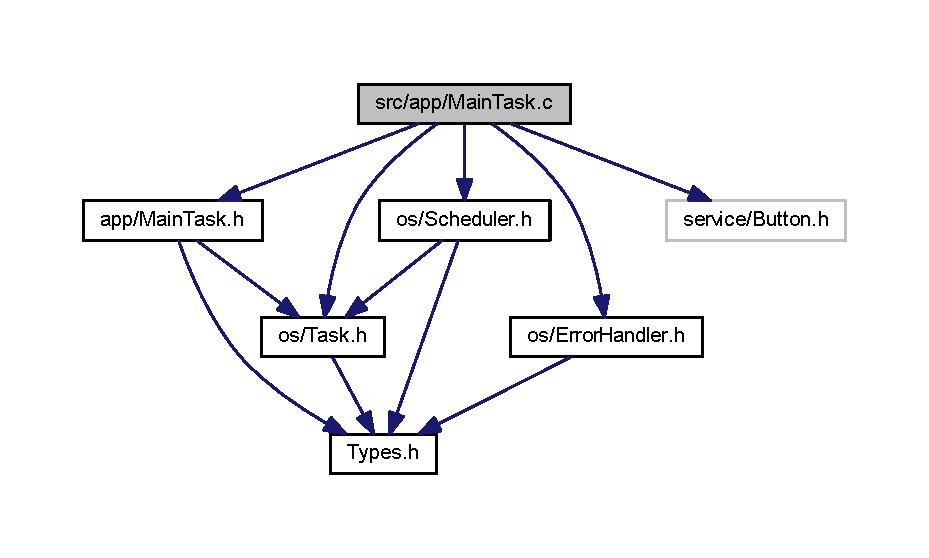
\includegraphics[width=350pt]{_main_task_8c__incl}
\end{center}
\end{figure}
\subsection*{Functions}
\begin{DoxyCompactItemize}
\item 
\hyperlink{_main_task_8h_a5c7f6fc98960ac3da07fc301f50b5e2f}{Main\+Task\+\_\+\+Ret} \hyperlink{_main_task_8c_a6184313b8eacbe1ebb0850cfc01c7d18}{Main\+Task\+\_\+init} (void)
\begin{DoxyCompactList}\small\item\em Initialize the main task. \end{DoxyCompactList}\end{DoxyCompactItemize}


\subsection{Detailed Description}
Main Application task. 

For a detailed description see the detailed description in \hyperlink{_main_task_8h}{Main\+Task.\+h}.

\begin{DoxyVersion}{Version}
\$\+Id\+: \hyperlink{_main_task_8c}{Main\+Task.\+c} 281 2024-\/01-\/12 12\+:09\+:03\+Z leglaz \$ 
\end{DoxyVersion}


\subsection{Function Documentation}
\hypertarget{_main_task_8c_a6184313b8eacbe1ebb0850cfc01c7d18}{\index{Main\+Task.\+c@{Main\+Task.\+c}!Main\+Task\+\_\+init@{Main\+Task\+\_\+init}}
\index{Main\+Task\+\_\+init@{Main\+Task\+\_\+init}!Main\+Task.\+c@{Main\+Task.\+c}}
\subsubsection[{Main\+Task\+\_\+init}]{\setlength{\rightskip}{0pt plus 5cm}{\bf Main\+Task\+\_\+\+Ret} Main\+Task\+\_\+init (
\begin{DoxyParamCaption}
\item[{void}]{}
\end{DoxyParamCaption}
)}}\label{_main_task_8c_a6184313b8eacbe1ebb0850cfc01c7d18}


Initialize the main task. 



References M\+A\+I\+N\+T\+A\+S\+K\+\_\+\+R\+E\+T\+\_\+\+A\+D\+D\+\_\+\+T\+A\+S\+K\+\_\+\+F\+A\+I\+L, M\+A\+I\+N\+T\+A\+S\+K\+\_\+\+R\+E\+T\+\_\+\+I\+N\+I\+T\+\_\+\+T\+A\+S\+K\+\_\+\+F\+A\+I\+L, M\+A\+I\+N\+T\+A\+S\+K\+\_\+\+R\+E\+T\+\_\+\+I\+N\+T\+E\+R\+N\+A\+L\+\_\+\+E\+R\+R\+O\+R, N\+U\+L\+L, Scheduler\+\_\+add\+Task(), S\+C\+H\+E\+D\+U\+L\+E\+R\+\_\+\+R\+E\+T\+\_\+\+S\+U\+C\+C\+E\+S\+S, Task\+\_\+init(), T\+A\+S\+K\+\_\+\+R\+E\+T\+\_\+\+S\+U\+C\+C\+E\+S\+S, and T\+A\+S\+K\+\_\+\+S\+T\+A\+T\+E\+\_\+\+R\+U\+N\+N\+I\+N\+G.



Here is the call graph for this function\+:\nopagebreak
\begin{figure}[H]
\begin{center}
\leavevmode
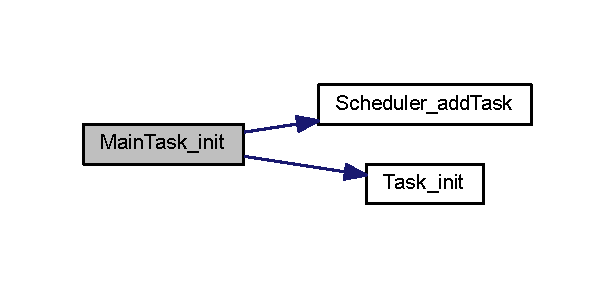
\includegraphics[width=295pt]{_main_task_8c_a6184313b8eacbe1ebb0850cfc01c7d18_cgraph}
\end{center}
\end{figure}



\hypertarget{_main_task_8h}{\section{src/app/\+Main\+Task.h File Reference}
\label{_main_task_8h}\index{src/app/\+Main\+Task.\+h@{src/app/\+Main\+Task.\+h}}
}


The main application task.  


{\ttfamily \#include \char`\"{}Types.\+h\char`\"{}}\\*
{\ttfamily \#include \char`\"{}os/\+Task.\+h\char`\"{}}\\*
Include dependency graph for Main\+Task.\+h\+:\nopagebreak
\begin{figure}[H]
\begin{center}
\leavevmode
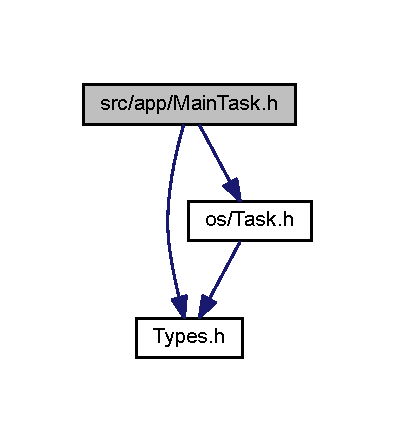
\includegraphics[width=190pt]{_main_task_8h__incl}
\end{center}
\end{figure}
This graph shows which files directly or indirectly include this file\+:\nopagebreak
\begin{figure}[H]
\begin{center}
\leavevmode
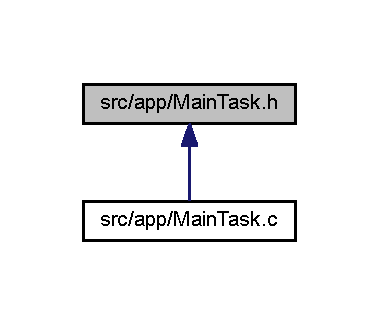
\includegraphics[width=182pt]{_main_task_8h__dep__incl}
\end{center}
\end{figure}
\subsection*{Enumerations}
\begin{DoxyCompactItemize}
\item 
enum \hyperlink{_main_task_8h_a5c7f6fc98960ac3da07fc301f50b5e2f}{Main\+Task\+\_\+\+Ret} \{ \hyperlink{_main_task_8h_a5c7f6fc98960ac3da07fc301f50b5e2fa0f8f7dc07e85f8a1c4f57e8fd0d39939}{M\+A\+I\+N\+T\+A\+S\+K\+\_\+\+R\+E\+T\+\_\+\+S\+U\+C\+C\+E\+S\+S} = 0, 
\hyperlink{_main_task_8h_a5c7f6fc98960ac3da07fc301f50b5e2fa0fb7c34347448a2bef05bcab5eee480c}{M\+A\+I\+N\+T\+A\+S\+K\+\_\+\+R\+E\+T\+\_\+\+I\+N\+I\+T\+\_\+\+T\+A\+S\+K\+\_\+\+F\+A\+I\+L}, 
\hyperlink{_main_task_8h_a5c7f6fc98960ac3da07fc301f50b5e2fa3fe7c66208c7817195196210efb61417}{M\+A\+I\+N\+T\+A\+S\+K\+\_\+\+R\+E\+T\+\_\+\+A\+D\+D\+\_\+\+T\+A\+S\+K\+\_\+\+F\+A\+I\+L}, 
\hyperlink{_main_task_8h_a5c7f6fc98960ac3da07fc301f50b5e2fa3066967e43ffd5681eb7153ff306b060}{M\+A\+I\+N\+T\+A\+S\+K\+\_\+\+R\+E\+T\+\_\+\+I\+N\+T\+E\+R\+N\+A\+L\+\_\+\+E\+R\+R\+O\+R}
 \}
\begin{DoxyCompactList}\small\item\em Statuses of the Main task. \end{DoxyCompactList}\end{DoxyCompactItemize}
\subsection*{Functions}
\begin{DoxyCompactItemize}
\item 
\hyperlink{_main_task_8h_a5c7f6fc98960ac3da07fc301f50b5e2f}{Main\+Task\+\_\+\+Ret} \hyperlink{_main_task_8h_a6184313b8eacbe1ebb0850cfc01c7d18}{Main\+Task\+\_\+init} (void)
\begin{DoxyCompactList}\small\item\em Initialize the main task. \end{DoxyCompactList}\end{DoxyCompactItemize}


\subsection{Detailed Description}
The main application task. 

\begin{DoxyVersion}{Version}
\$\+Id\+: \hyperlink{_main_task_8h}{Main\+Task.\+h} 281 2024-\/01-\/12 12\+:09\+:03\+Z leglaz \$ 
\end{DoxyVersion}


\subsection{Enumeration Type Documentation}
\hypertarget{_main_task_8h_a5c7f6fc98960ac3da07fc301f50b5e2f}{\index{Main\+Task.\+h@{Main\+Task.\+h}!Main\+Task\+\_\+\+Ret@{Main\+Task\+\_\+\+Ret}}
\index{Main\+Task\+\_\+\+Ret@{Main\+Task\+\_\+\+Ret}!Main\+Task.\+h@{Main\+Task.\+h}}
\subsubsection[{Main\+Task\+\_\+\+Ret}]{\setlength{\rightskip}{0pt plus 5cm}enum {\bf Main\+Task\+\_\+\+Ret}}}\label{_main_task_8h_a5c7f6fc98960ac3da07fc301f50b5e2f}


Statuses of the Main task. 

\begin{Desc}
\item[Enumerator]\par
\begin{description}
\index{M\+A\+I\+N\+T\+A\+S\+K\+\_\+\+R\+E\+T\+\_\+\+S\+U\+C\+C\+E\+S\+S@{M\+A\+I\+N\+T\+A\+S\+K\+\_\+\+R\+E\+T\+\_\+\+S\+U\+C\+C\+E\+S\+S}!Main\+Task.\+h@{Main\+Task.\+h}}\index{Main\+Task.\+h@{Main\+Task.\+h}!M\+A\+I\+N\+T\+A\+S\+K\+\_\+\+R\+E\+T\+\_\+\+S\+U\+C\+C\+E\+S\+S@{M\+A\+I\+N\+T\+A\+S\+K\+\_\+\+R\+E\+T\+\_\+\+S\+U\+C\+C\+E\+S\+S}}\item[{\em 
\hypertarget{_main_task_8h_a5c7f6fc98960ac3da07fc301f50b5e2fa0f8f7dc07e85f8a1c4f57e8fd0d39939}{M\+A\+I\+N\+T\+A\+S\+K\+\_\+\+R\+E\+T\+\_\+\+S\+U\+C\+C\+E\+S\+S}\label{_main_task_8h_a5c7f6fc98960ac3da07fc301f50b5e2fa0f8f7dc07e85f8a1c4f57e8fd0d39939}
}]Ok. \index{M\+A\+I\+N\+T\+A\+S\+K\+\_\+\+R\+E\+T\+\_\+\+I\+N\+I\+T\+\_\+\+T\+A\+S\+K\+\_\+\+F\+A\+I\+L@{M\+A\+I\+N\+T\+A\+S\+K\+\_\+\+R\+E\+T\+\_\+\+I\+N\+I\+T\+\_\+\+T\+A\+S\+K\+\_\+\+F\+A\+I\+L}!Main\+Task.\+h@{Main\+Task.\+h}}\index{Main\+Task.\+h@{Main\+Task.\+h}!M\+A\+I\+N\+T\+A\+S\+K\+\_\+\+R\+E\+T\+\_\+\+I\+N\+I\+T\+\_\+\+T\+A\+S\+K\+\_\+\+F\+A\+I\+L@{M\+A\+I\+N\+T\+A\+S\+K\+\_\+\+R\+E\+T\+\_\+\+I\+N\+I\+T\+\_\+\+T\+A\+S\+K\+\_\+\+F\+A\+I\+L}}\item[{\em 
\hypertarget{_main_task_8h_a5c7f6fc98960ac3da07fc301f50b5e2fa0fb7c34347448a2bef05bcab5eee480c}{M\+A\+I\+N\+T\+A\+S\+K\+\_\+\+R\+E\+T\+\_\+\+I\+N\+I\+T\+\_\+\+T\+A\+S\+K\+\_\+\+F\+A\+I\+L}\label{_main_task_8h_a5c7f6fc98960ac3da07fc301f50b5e2fa0fb7c34347448a2bef05bcab5eee480c}
}]Initalization failed. \index{M\+A\+I\+N\+T\+A\+S\+K\+\_\+\+R\+E\+T\+\_\+\+A\+D\+D\+\_\+\+T\+A\+S\+K\+\_\+\+F\+A\+I\+L@{M\+A\+I\+N\+T\+A\+S\+K\+\_\+\+R\+E\+T\+\_\+\+A\+D\+D\+\_\+\+T\+A\+S\+K\+\_\+\+F\+A\+I\+L}!Main\+Task.\+h@{Main\+Task.\+h}}\index{Main\+Task.\+h@{Main\+Task.\+h}!M\+A\+I\+N\+T\+A\+S\+K\+\_\+\+R\+E\+T\+\_\+\+A\+D\+D\+\_\+\+T\+A\+S\+K\+\_\+\+F\+A\+I\+L@{M\+A\+I\+N\+T\+A\+S\+K\+\_\+\+R\+E\+T\+\_\+\+A\+D\+D\+\_\+\+T\+A\+S\+K\+\_\+\+F\+A\+I\+L}}\item[{\em 
\hypertarget{_main_task_8h_a5c7f6fc98960ac3da07fc301f50b5e2fa3fe7c66208c7817195196210efb61417}{M\+A\+I\+N\+T\+A\+S\+K\+\_\+\+R\+E\+T\+\_\+\+A\+D\+D\+\_\+\+T\+A\+S\+K\+\_\+\+F\+A\+I\+L}\label{_main_task_8h_a5c7f6fc98960ac3da07fc301f50b5e2fa3fe7c66208c7817195196210efb61417}
}]Adding failed. \index{M\+A\+I\+N\+T\+A\+S\+K\+\_\+\+R\+E\+T\+\_\+\+I\+N\+T\+E\+R\+N\+A\+L\+\_\+\+E\+R\+R\+O\+R@{M\+A\+I\+N\+T\+A\+S\+K\+\_\+\+R\+E\+T\+\_\+\+I\+N\+T\+E\+R\+N\+A\+L\+\_\+\+E\+R\+R\+O\+R}!Main\+Task.\+h@{Main\+Task.\+h}}\index{Main\+Task.\+h@{Main\+Task.\+h}!M\+A\+I\+N\+T\+A\+S\+K\+\_\+\+R\+E\+T\+\_\+\+I\+N\+T\+E\+R\+N\+A\+L\+\_\+\+E\+R\+R\+O\+R@{M\+A\+I\+N\+T\+A\+S\+K\+\_\+\+R\+E\+T\+\_\+\+I\+N\+T\+E\+R\+N\+A\+L\+\_\+\+E\+R\+R\+O\+R}}\item[{\em 
\hypertarget{_main_task_8h_a5c7f6fc98960ac3da07fc301f50b5e2fa3066967e43ffd5681eb7153ff306b060}{M\+A\+I\+N\+T\+A\+S\+K\+\_\+\+R\+E\+T\+\_\+\+I\+N\+T\+E\+R\+N\+A\+L\+\_\+\+E\+R\+R\+O\+R}\label{_main_task_8h_a5c7f6fc98960ac3da07fc301f50b5e2fa3066967e43ffd5681eb7153ff306b060}
}]Internal error. \end{description}
\end{Desc}


\subsection{Function Documentation}
\hypertarget{_main_task_8h_a6184313b8eacbe1ebb0850cfc01c7d18}{\index{Main\+Task.\+h@{Main\+Task.\+h}!Main\+Task\+\_\+init@{Main\+Task\+\_\+init}}
\index{Main\+Task\+\_\+init@{Main\+Task\+\_\+init}!Main\+Task.\+h@{Main\+Task.\+h}}
\subsubsection[{Main\+Task\+\_\+init}]{\setlength{\rightskip}{0pt plus 5cm}{\bf Main\+Task\+\_\+\+Ret} Main\+Task\+\_\+init (
\begin{DoxyParamCaption}
\item[{void}]{}
\end{DoxyParamCaption}
)}}\label{_main_task_8h_a6184313b8eacbe1ebb0850cfc01c7d18}


Initialize the main task. 



References M\+A\+I\+N\+T\+A\+S\+K\+\_\+\+R\+E\+T\+\_\+\+A\+D\+D\+\_\+\+T\+A\+S\+K\+\_\+\+F\+A\+I\+L, M\+A\+I\+N\+T\+A\+S\+K\+\_\+\+R\+E\+T\+\_\+\+I\+N\+I\+T\+\_\+\+T\+A\+S\+K\+\_\+\+F\+A\+I\+L, M\+A\+I\+N\+T\+A\+S\+K\+\_\+\+R\+E\+T\+\_\+\+I\+N\+T\+E\+R\+N\+A\+L\+\_\+\+E\+R\+R\+O\+R, N\+U\+L\+L, Scheduler\+\_\+add\+Task(), S\+C\+H\+E\+D\+U\+L\+E\+R\+\_\+\+R\+E\+T\+\_\+\+S\+U\+C\+C\+E\+S\+S, Task\+\_\+init(), T\+A\+S\+K\+\_\+\+R\+E\+T\+\_\+\+S\+U\+C\+C\+E\+S\+S, and T\+A\+S\+K\+\_\+\+S\+T\+A\+T\+E\+\_\+\+R\+U\+N\+N\+I\+N\+G.



Here is the call graph for this function\+:\nopagebreak
\begin{figure}[H]
\begin{center}
\leavevmode
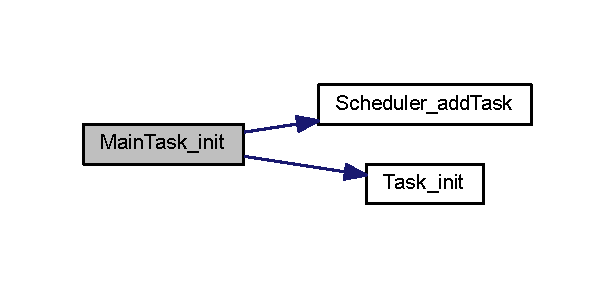
\includegraphics[width=295pt]{_main_task_8h_a6184313b8eacbe1ebb0850cfc01c7d18_cgraph}
\end{center}
\end{figure}



\hypertarget{_types_8h}{\section{src/\+Common/\+Types.h File Reference}
\label{_types_8h}\index{src/\+Common/\+Types.\+h@{src/\+Common/\+Types.\+h}}
}


Basic types definition for A\+Tmega128.  


This graph shows which files directly or indirectly include this file\+:\nopagebreak
\begin{figure}[H]
\begin{center}
\leavevmode
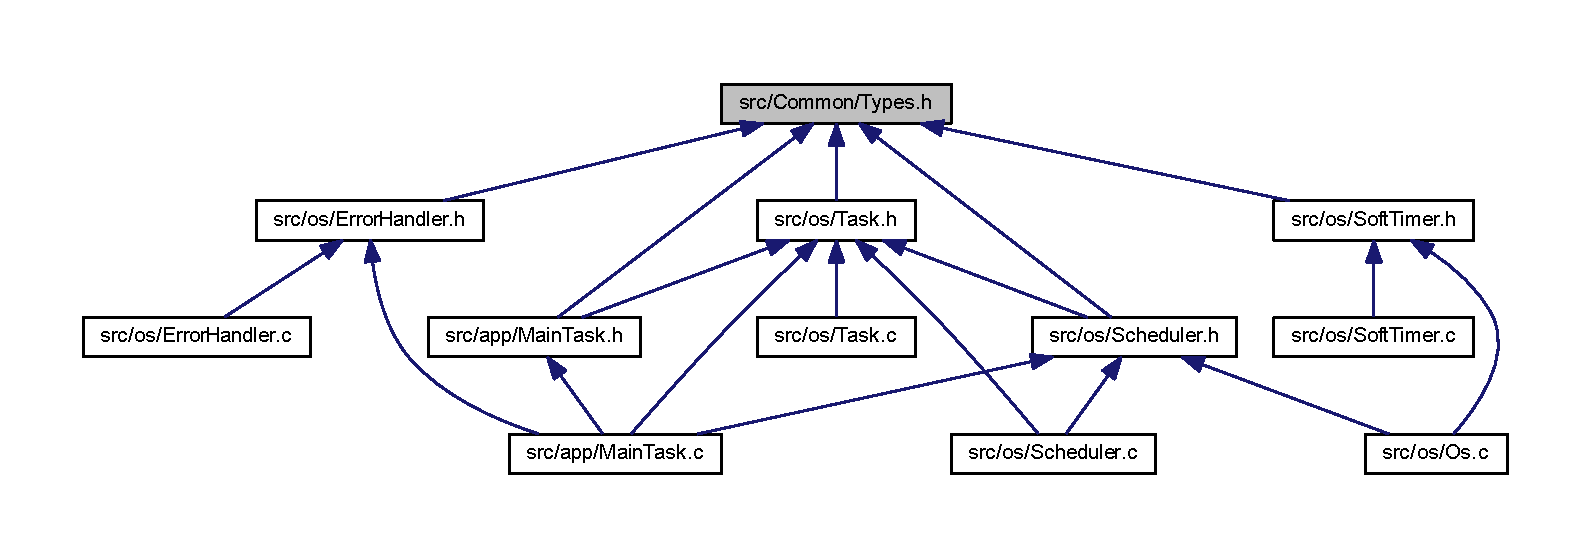
\includegraphics[width=350pt]{_types_8h__dep__incl}
\end{center}
\end{figure}
\subsection*{Macros}
\begin{DoxyCompactItemize}
\item 
\hypertarget{_types_8h_a070d2ce7b6bb7e5c05602aa8c308d0c4}{\#define \hyperlink{_types_8h_a070d2ce7b6bb7e5c05602aa8c308d0c4}{N\+U\+L\+L}~((void $\ast$) 0)}\label{_types_8h_a070d2ce7b6bb7e5c05602aa8c308d0c4}

\begin{DoxyCompactList}\small\item\em N\+U\+L\+L. \end{DoxyCompactList}\end{DoxyCompactItemize}
\subsection*{Typedefs}
\begin{DoxyCompactItemize}
\item 
\hypertarget{_types_8h_ae3a497195d617519e5353ea7b417940f}{typedef unsigned char \hyperlink{_types_8h_ae3a497195d617519e5353ea7b417940f}{Byte}}\label{_types_8h_ae3a497195d617519e5353ea7b417940f}

\begin{DoxyCompactList}\small\item\em 8\+Bit data type \end{DoxyCompactList}\item 
\hypertarget{_types_8h_a5a0fa7fd26bf95968c50ea6c1dc48825}{typedef unsigned char \hyperlink{_types_8h_a5a0fa7fd26bf95968c50ea6c1dc48825}{U\+Char}}\label{_types_8h_a5a0fa7fd26bf95968c50ea6c1dc48825}

\begin{DoxyCompactList}\small\item\em 8\+Bit character A\+S\+C\+I\+I256 \end{DoxyCompactList}\item 
\hypertarget{_types_8h_aa141593bc2edcab4eba2fb880aad19b2}{typedef signed char \hyperlink{_types_8h_aa141593bc2edcab4eba2fb880aad19b2}{Char}}\label{_types_8h_aa141593bc2edcab4eba2fb880aad19b2}

\begin{DoxyCompactList}\small\item\em 8\+Bit character A\+S\+C\+I\+I128 \end{DoxyCompactList}\item 
\hypertarget{_types_8h_a7e31ca7716b8d85dd473450a5c5e5a97}{typedef signed char \hyperlink{_types_8h_a7e31ca7716b8d85dd473450a5c5e5a97}{Int8}}\label{_types_8h_a7e31ca7716b8d85dd473450a5c5e5a97}

\begin{DoxyCompactList}\small\item\em 8\+Bit signed integer \end{DoxyCompactList}\item 
\hypertarget{_types_8h_a9b66271558bfa5abc5095791246b540d}{typedef unsigned char \hyperlink{_types_8h_a9b66271558bfa5abc5095791246b540d}{U\+Int8}}\label{_types_8h_a9b66271558bfa5abc5095791246b540d}

\begin{DoxyCompactList}\small\item\em 8\+Bit unsigned integer \end{DoxyCompactList}\item 
\hypertarget{_types_8h_a6848f29a2fa83032f12605820b27b9f0}{typedef volatile unsigned char \hyperlink{_types_8h_a6848f29a2fa83032f12605820b27b9f0}{V\+U\+Int8}}\label{_types_8h_a6848f29a2fa83032f12605820b27b9f0}

\begin{DoxyCompactList}\small\item\em 8\+Bit volatile unsigned integer \end{DoxyCompactList}\item 
\hypertarget{_types_8h_a47bfd492cc0c523df1f3b5e4c749156e}{typedef volatile signed char \hyperlink{_types_8h_a47bfd492cc0c523df1f3b5e4c749156e}{V\+Int8}}\label{_types_8h_a47bfd492cc0c523df1f3b5e4c749156e}

\begin{DoxyCompactList}\small\item\em 8\+Bit volatile integer \end{DoxyCompactList}\item 
\hypertarget{_types_8h_a659ce9e5eb6571f9984ffc7caad2660a}{typedef signed int \hyperlink{_types_8h_a659ce9e5eb6571f9984ffc7caad2660a}{Int16}}\label{_types_8h_a659ce9e5eb6571f9984ffc7caad2660a}

\begin{DoxyCompactList}\small\item\em 16\+Bit signed integer \end{DoxyCompactList}\item 
\hypertarget{_types_8h_aad0fc9943ec46ed9388d30c8ebe52b77}{typedef unsigned int \hyperlink{_types_8h_aad0fc9943ec46ed9388d30c8ebe52b77}{U\+Int16}}\label{_types_8h_aad0fc9943ec46ed9388d30c8ebe52b77}

\begin{DoxyCompactList}\small\item\em 16\+Bit unsigned integer \end{DoxyCompactList}\item 
\hypertarget{_types_8h_ae10a43dba9efad58e7c36513375ba0f9}{typedef volatile unsigned int \hyperlink{_types_8h_ae10a43dba9efad58e7c36513375ba0f9}{V\+U\+Int16}}\label{_types_8h_ae10a43dba9efad58e7c36513375ba0f9}

\begin{DoxyCompactList}\small\item\em 16\+Bit volatile unsigned integer \end{DoxyCompactList}\item 
\hypertarget{_types_8h_ab14c94b9f07750cee9b162c101ee68f5}{typedef volatile signed int \hyperlink{_types_8h_ab14c94b9f07750cee9b162c101ee68f5}{V\+Int16}}\label{_types_8h_ab14c94b9f07750cee9b162c101ee68f5}

\begin{DoxyCompactList}\small\item\em 16\+Bit volatile unsigned integer \end{DoxyCompactList}\item 
\hypertarget{_types_8h_a184d0ff2424cf4b81c68ce9538481a04}{typedef signed long \hyperlink{_types_8h_a184d0ff2424cf4b81c68ce9538481a04}{Int32}}\label{_types_8h_a184d0ff2424cf4b81c68ce9538481a04}

\begin{DoxyCompactList}\small\item\em 32\+Bit signed integer \end{DoxyCompactList}\item 
\hypertarget{_types_8h_aff6f5ee5b7d4f374428d4a853d976f94}{typedef unsigned long \hyperlink{_types_8h_aff6f5ee5b7d4f374428d4a853d976f94}{U\+Int32}}\label{_types_8h_aff6f5ee5b7d4f374428d4a853d976f94}

\begin{DoxyCompactList}\small\item\em 32\+Bit unsigned integer \end{DoxyCompactList}\item 
\hypertarget{_types_8h_ae63080690e6ebce3fd1b7b9a1ead4b98}{typedef volatile unsigned long \hyperlink{_types_8h_ae63080690e6ebce3fd1b7b9a1ead4b98}{V\+U\+Int32}}\label{_types_8h_ae63080690e6ebce3fd1b7b9a1ead4b98}

\begin{DoxyCompactList}\small\item\em 32\+Bit volatile unsigned integer \end{DoxyCompactList}\item 
\hypertarget{_types_8h_a41ac7dbc589c972dd189993b87273336}{typedef volatile signed long \hyperlink{_types_8h_a41ac7dbc589c972dd189993b87273336}{V\+Int32}}\label{_types_8h_a41ac7dbc589c972dd189993b87273336}

\begin{DoxyCompactList}\small\item\em 32\+Bit volatile unsigned integer \end{DoxyCompactList}\item 
\hypertarget{_types_8h_a56afe571a9be7582d493be2b31aed0ea}{typedef signed long long \hyperlink{_types_8h_a56afe571a9be7582d493be2b31aed0ea}{Int64}}\label{_types_8h_a56afe571a9be7582d493be2b31aed0ea}

\begin{DoxyCompactList}\small\item\em 64\+Bit signed integer \end{DoxyCompactList}\item 
\hypertarget{_types_8h_aa1d7d331b6d522d6d9840fece27108d8}{typedef unsigned long long \hyperlink{_types_8h_aa1d7d331b6d522d6d9840fece27108d8}{U\+Int64}}\label{_types_8h_aa1d7d331b6d522d6d9840fece27108d8}

\begin{DoxyCompactList}\small\item\em 64\+Bit unsigned integer \end{DoxyCompactList}\item 
\hypertarget{_types_8h_a39add53053b29a922c621524b5fdbbc9}{typedef volatile unsigned long long \hyperlink{_types_8h_a39add53053b29a922c621524b5fdbbc9}{V\+U\+Int64}}\label{_types_8h_a39add53053b29a922c621524b5fdbbc9}

\begin{DoxyCompactList}\small\item\em 64\+Bit volatile unsigned integer \end{DoxyCompactList}\item 
\hypertarget{_types_8h_acc0858a2f0a3df5399e5d7b963eb5241}{typedef volatile signed long long \hyperlink{_types_8h_acc0858a2f0a3df5399e5d7b963eb5241}{V\+Int64}}\label{_types_8h_acc0858a2f0a3df5399e5d7b963eb5241}

\begin{DoxyCompactList}\small\item\em 64\+Bit volatile unsigned integer \end{DoxyCompactList}\item 
\hypertarget{_types_8h_a87d38f886e617ced2698fc55afa07637}{typedef float \hyperlink{_types_8h_a87d38f886e617ced2698fc55afa07637}{Float32}}\label{_types_8h_a87d38f886e617ced2698fc55afa07637}

\begin{DoxyCompactList}\small\item\em 32\+Bit floating point \end{DoxyCompactList}\item 
\hypertarget{_types_8h_a81c86892a6bccf31d9154453da060386}{typedef volatile float \hyperlink{_types_8h_a81c86892a6bccf31d9154453da060386}{V\+Float32}}\label{_types_8h_a81c86892a6bccf31d9154453da060386}

\begin{DoxyCompactList}\small\item\em 32\+Bit floating point \end{DoxyCompactList}\item 
\hypertarget{_types_8h_ac618847877068404a9c47b29e51f6cda}{typedef long double \hyperlink{_types_8h_ac618847877068404a9c47b29e51f6cda}{Float64}}\label{_types_8h_ac618847877068404a9c47b29e51f6cda}

\begin{DoxyCompactList}\small\item\em 32\+Bit floating point \end{DoxyCompactList}\item 
\hypertarget{_types_8h_ab63916734ec8149263baae3331375fa4}{typedef volatile long double \hyperlink{_types_8h_ab63916734ec8149263baae3331375fa4}{V\+Float64}}\label{_types_8h_ab63916734ec8149263baae3331375fa4}

\begin{DoxyCompactList}\small\item\em 32\+Bit floating point \end{DoxyCompactList}\item 
\hypertarget{_types_8h_acb2cafebbc492a8f4e0758e9cd14a623}{typedef \hyperlink{_types_8h_a6848f29a2fa83032f12605820b27b9f0}{V\+U\+Int8} \hyperlink{_types_8h_acb2cafebbc492a8f4e0758e9cd14a623}{Reg8}}\label{_types_8h_acb2cafebbc492a8f4e0758e9cd14a623}

\begin{DoxyCompactList}\small\item\em 8\+Bit register \end{DoxyCompactList}\item 
\hypertarget{_types_8h_a347323846f4104fb7393e9aa6c0e4ef4}{typedef \hyperlink{_types_8h_ae10a43dba9efad58e7c36513375ba0f9}{V\+U\+Int16} \hyperlink{_types_8h_a347323846f4104fb7393e9aa6c0e4ef4}{Reg16}}\label{_types_8h_a347323846f4104fb7393e9aa6c0e4ef4}

\begin{DoxyCompactList}\small\item\em 16\+Bit register \end{DoxyCompactList}\item 
\hypertarget{_types_8h_a88f9ce72faa4a644db59b0880bf2b0ff}{typedef \hyperlink{_types_8h_ae63080690e6ebce3fd1b7b9a1ead4b98}{V\+U\+Int32} \hyperlink{_types_8h_a88f9ce72faa4a644db59b0880bf2b0ff}{Reg32}}\label{_types_8h_a88f9ce72faa4a644db59b0880bf2b0ff}

\begin{DoxyCompactList}\small\item\em 32\+Bit register \end{DoxyCompactList}\item 
\hypertarget{_types_8h_ae95f4e33ca147189a6cf24a018a2e00b}{typedef \hyperlink{_types_8h_a39add53053b29a922c621524b5fdbbc9}{V\+U\+Int64} \hyperlink{_types_8h_ae95f4e33ca147189a6cf24a018a2e00b}{Reg64}}\label{_types_8h_ae95f4e33ca147189a6cf24a018a2e00b}

\begin{DoxyCompactList}\small\item\em 64\+Bit register \end{DoxyCompactList}\end{DoxyCompactItemize}
\subsection*{Enumerations}
\begin{DoxyCompactItemize}
\item 
\hypertarget{_types_8h_a39db6982619d623273fad8a383489309}{enum \hyperlink{_types_8h_a39db6982619d623273fad8a383489309}{Bool} \{ {\bfseries F\+A\+L\+S\+E} = 0, 
{\bfseries T\+R\+U\+E} = 1
 \}}\label{_types_8h_a39db6982619d623273fad8a383489309}

\begin{DoxyCompactList}\small\item\em Boolean data type. \end{DoxyCompactList}\end{DoxyCompactItemize}


\subsection{Detailed Description}
Basic types definition for A\+Tmega128. 

\begin{DoxyVersion}{Version}
\$\+Id\+: \hyperlink{_types_8h}{Types.\+h} 281 2024-\/01-\/12 12\+:09\+:03\+Z leglaz \$ 
\end{DoxyVersion}

\hypertarget{_error_handler_8c}{\section{src/os/\+Error\+Handler.c File Reference}
\label{_error_handler_8c}\index{src/os/\+Error\+Handler.\+c@{src/os/\+Error\+Handler.\+c}}
}


Error\+Handler for all error processing.  


{\ttfamily \#include \char`\"{}os/\+Error\+Handler.\+h\char`\"{}}\\*
{\ttfamily \#include \char`\"{}hal/\+Hal.\+h\char`\"{}}\\*
Include dependency graph for Error\+Handler.\+c\+:\nopagebreak
\begin{figure}[H]
\begin{center}
\leavevmode
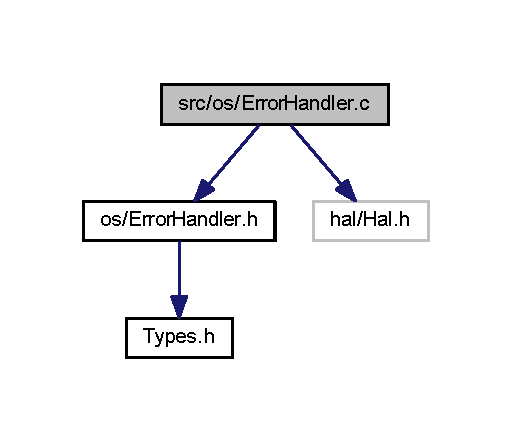
\includegraphics[width=246pt]{_error_handler_8c__incl}
\end{center}
\end{figure}
\subsection*{Functions}
\begin{DoxyCompactItemize}
\item 
void \hyperlink{_error_handler_8c_acc05881f1c6f1090dd9d1d88d32e2d88}{Error\+Handler\+\_\+set\+Print\+Callback} (\hyperlink{_error_handler_8h_a675699c57a733118f4641f24541892aa}{Print\+Callback} callback)
\begin{DoxyCompactList}\small\item\em Install error message output handler via callback interface. \end{DoxyCompactList}\item 
void \hyperlink{_error_handler_8c_a7acf566cf4c47dc7d15895e92608eda9}{Error\+Handler\+\_\+set\+Error\+Callback} (\hyperlink{_error_handler_8h_a2e96a0567c5de834b9d8fcfe70c2cc55}{Error\+Callback} callback)
\begin{DoxyCompactList}\small\item\em Install application error handler. \end{DoxyCompactList}\item 
void \hyperlink{_error_handler_8c_a9356b0c8efca0c26f7b118582087e9e3}{Error\+Handler\+\_\+show} (\hyperlink{_error_handler_8h_aed7d97b22f3571652032b3136460f314}{Error\+Handler\+Error\+Code} error\+Code)
\begin{DoxyCompactList}\small\item\em Show error code and return. \end{DoxyCompactList}\item 
void \hyperlink{_error_handler_8c_a7a5a812a13a9c76e57887ce64ddd7e18}{Error\+Handler\+\_\+halt} (\hyperlink{_error_handler_8h_aed7d97b22f3571652032b3136460f314}{Error\+Handler\+Error\+Code} error\+Code)
\begin{DoxyCompactList}\small\item\em Show error code and halt system. \end{DoxyCompactList}\end{DoxyCompactItemize}


\subsection{Detailed Description}
Error\+Handler for all error processing. 

\begin{DoxyVersion}{Version}
\$\+Id\+: \hyperlink{_error_handler_8c}{Error\+Handler.\+c} 294 2024-\/01-\/30 10\+:28\+:46\+Z leglaz \$ 
\end{DoxyVersion}


\subsection{Function Documentation}
\hypertarget{_error_handler_8c_a7a5a812a13a9c76e57887ce64ddd7e18}{\index{Error\+Handler.\+c@{Error\+Handler.\+c}!Error\+Handler\+\_\+halt@{Error\+Handler\+\_\+halt}}
\index{Error\+Handler\+\_\+halt@{Error\+Handler\+\_\+halt}!Error\+Handler.\+c@{Error\+Handler.\+c}}
\subsubsection[{Error\+Handler\+\_\+halt}]{\setlength{\rightskip}{0pt plus 5cm}void Error\+Handler\+\_\+halt (
\begin{DoxyParamCaption}
\item[{{\bf Error\+Handler\+Error\+Code}}]{error\+Code}
\end{DoxyParamCaption}
)}}\label{_error_handler_8c_a7a5a812a13a9c76e57887ce64ddd7e18}


Show error code and halt system. 


\begin{DoxyParams}[1]{Parameters}
\mbox{\tt in}  & {\em error\+Code} & Numeric error code to display. \\
\hline
\end{DoxyParams}
\hypertarget{_error_handler_8c_a7acf566cf4c47dc7d15895e92608eda9}{\index{Error\+Handler.\+c@{Error\+Handler.\+c}!Error\+Handler\+\_\+set\+Error\+Callback@{Error\+Handler\+\_\+set\+Error\+Callback}}
\index{Error\+Handler\+\_\+set\+Error\+Callback@{Error\+Handler\+\_\+set\+Error\+Callback}!Error\+Handler.\+c@{Error\+Handler.\+c}}
\subsubsection[{Error\+Handler\+\_\+set\+Error\+Callback}]{\setlength{\rightskip}{0pt plus 5cm}void Error\+Handler\+\_\+set\+Error\+Callback (
\begin{DoxyParamCaption}
\item[{{\bf Error\+Callback}}]{callback}
\end{DoxyParamCaption}
)}}\label{_error_handler_8c_a7acf566cf4c47dc7d15895e92608eda9}


Install application error handler. 


\begin{DoxyParams}[1]{Parameters}
\mbox{\tt in}  & {\em callback} & callback function error handling. \\
\hline
\end{DoxyParams}
\hypertarget{_error_handler_8c_acc05881f1c6f1090dd9d1d88d32e2d88}{\index{Error\+Handler.\+c@{Error\+Handler.\+c}!Error\+Handler\+\_\+set\+Print\+Callback@{Error\+Handler\+\_\+set\+Print\+Callback}}
\index{Error\+Handler\+\_\+set\+Print\+Callback@{Error\+Handler\+\_\+set\+Print\+Callback}!Error\+Handler.\+c@{Error\+Handler.\+c}}
\subsubsection[{Error\+Handler\+\_\+set\+Print\+Callback}]{\setlength{\rightskip}{0pt plus 5cm}void Error\+Handler\+\_\+set\+Print\+Callback (
\begin{DoxyParamCaption}
\item[{{\bf Print\+Callback}}]{callback}
\end{DoxyParamCaption}
)}}\label{_error_handler_8c_acc05881f1c6f1090dd9d1d88d32e2d88}


Install error message output handler via callback interface. 


\begin{DoxyParams}[1]{Parameters}
\mbox{\tt in}  & {\em callback} & callback function for displaying error message. \\
\hline
\end{DoxyParams}
\hypertarget{_error_handler_8c_a9356b0c8efca0c26f7b118582087e9e3}{\index{Error\+Handler.\+c@{Error\+Handler.\+c}!Error\+Handler\+\_\+show@{Error\+Handler\+\_\+show}}
\index{Error\+Handler\+\_\+show@{Error\+Handler\+\_\+show}!Error\+Handler.\+c@{Error\+Handler.\+c}}
\subsubsection[{Error\+Handler\+\_\+show}]{\setlength{\rightskip}{0pt plus 5cm}void Error\+Handler\+\_\+show (
\begin{DoxyParamCaption}
\item[{{\bf Error\+Handler\+Error\+Code}}]{error\+Code}
\end{DoxyParamCaption}
)}}\label{_error_handler_8c_a9356b0c8efca0c26f7b118582087e9e3}


Show error code and return. 


\begin{DoxyParams}[1]{Parameters}
\mbox{\tt in}  & {\em error\+Code} & Numeric error code to display. \\
\hline
\end{DoxyParams}

\hypertarget{_error_handler_8h}{\section{src/os/\+Error\+Handler.h File Reference}
\label{_error_handler_8h}\index{src/os/\+Error\+Handler.\+h@{src/os/\+Error\+Handler.\+h}}
}


Enter short description here.  


{\ttfamily \#include \char`\"{}Types.\+h\char`\"{}}\\*
Include dependency graph for Error\+Handler.\+h\+:\nopagebreak
\begin{figure}[H]
\begin{center}
\leavevmode
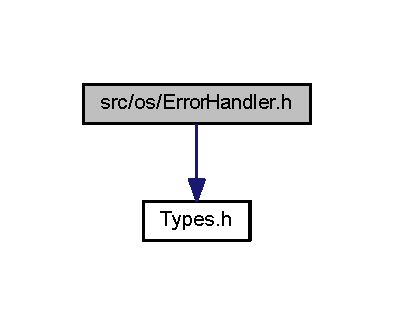
\includegraphics[width=189pt]{_error_handler_8h__incl}
\end{center}
\end{figure}
This graph shows which files directly or indirectly include this file\+:\nopagebreak
\begin{figure}[H]
\begin{center}
\leavevmode
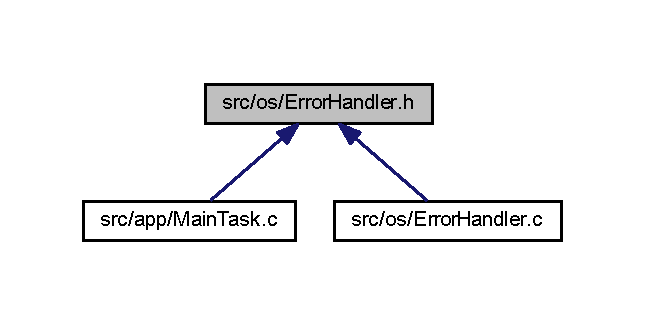
\includegraphics[width=310pt]{_error_handler_8h__dep__incl}
\end{center}
\end{figure}
\subsection*{Typedefs}
\begin{DoxyCompactItemize}
\item 
typedef enum \hyperlink{_error_handler_8h_ad1141f86ec521af1f274aeb9b73a7480}{tag\+\_\+\+Error\+Code} \hyperlink{_error_handler_8h_aed7d97b22f3571652032b3136460f314}{Error\+Handler\+Error\+Code}
\begin{DoxyCompactList}\small\item\em All error codes. \end{DoxyCompactList}\item 
typedef void($\ast$ \hyperlink{_error_handler_8h_a675699c57a733118f4641f24541892aa}{Print\+Callback} )(const char $\ast$line1, const char $\ast$line2)
\begin{DoxyCompactList}\small\item\em Callback function type for showing errror codes \char`\"{}somewhere\char`\"{}. \end{DoxyCompactList}\item 
\hypertarget{_error_handler_8h_a2e96a0567c5de834b9d8fcfe70c2cc55}{typedef void($\ast$ \hyperlink{_error_handler_8h_a2e96a0567c5de834b9d8fcfe70c2cc55}{Error\+Callback} )(\hyperlink{_error_handler_8h_aed7d97b22f3571652032b3136460f314}{Error\+Handler\+Error\+Code} errorcode)}\label{_error_handler_8h_a2e96a0567c5de834b9d8fcfe70c2cc55}

\begin{DoxyCompactList}\small\item\em Callback function type for app specific error handling. \end{DoxyCompactList}\end{DoxyCompactItemize}
\subsection*{Enumerations}
\begin{DoxyCompactItemize}
\item 
enum \hyperlink{_error_handler_8h_ad1141f86ec521af1f274aeb9b73a7480}{tag\+\_\+\+Error\+Code} \{ \\*
\hyperlink{_error_handler_8h_ad1141f86ec521af1f274aeb9b73a7480ab24e43d2d31b755eb736c4846dbac6de}{E\+R\+R\+O\+R\+H\+A\+N\+D\+L\+E\+R\+\_\+\+M\+A\+I\+N\+\_\+\+S\+C\+H\+E\+D\+U\+L\+E\+R\+\_\+\+E\+X\+I\+T} = 1, 
\hyperlink{_error_handler_8h_ad1141f86ec521af1f274aeb9b73a7480ae7049eee5952a4e52b1cd9329c41af0e}{E\+R\+R\+O\+R\+H\+A\+N\+D\+L\+E\+R\+\_\+\+M\+A\+I\+N\+T\+A\+S\+K\+\_\+\+I\+N\+I\+T\+\_\+\+F\+A\+I\+L} = 100, 
\hyperlink{_error_handler_8h_ad1141f86ec521af1f274aeb9b73a7480a3b616e54406bc97e2bec31267fd58b77}{E\+R\+R\+O\+R\+H\+A\+N\+D\+L\+E\+R\+\_\+\+S\+T\+A\+R\+T\+U\+P\+\_\+\+I\+N\+I\+T\+\_\+\+F\+A\+I\+L} = 110, 
\hyperlink{_error_handler_8h_ad1141f86ec521af1f274aeb9b73a7480a4b16e262ad88b9d9e5d0c761e4305a8e}{E\+R\+R\+O\+R\+H\+A\+N\+D\+L\+E\+R\+\_\+\+S\+T\+A\+R\+T\+U\+P\+\_\+\+U\+N\+I\+N\+I\+T\+\_\+\+F\+A\+I\+L} = 111, 
\\*
\hyperlink{_error_handler_8h_ad1141f86ec521af1f274aeb9b73a7480af34d5c411ff67c67f3d9e7c2b4a98b1b}{E\+R\+R\+O\+R\+H\+A\+N\+D\+L\+E\+R\+\_\+\+C\+A\+L\+I\+B\+R\+A\+T\+E\+\_\+\+T\+I\+M\+E\+R\+\_\+\+I\+N\+I\+T\+\_\+\+F\+A\+I\+L} = 200, 
\hyperlink{_error_handler_8h_ad1141f86ec521af1f274aeb9b73a7480a2678e9801b48c03ecce001f65ed34dd5}{E\+R\+R\+O\+R\+H\+A\+N\+D\+L\+E\+R\+\_\+\+C\+A\+L\+I\+B\+R\+A\+T\+E\+\_\+\+A\+L\+O\+G\+R\+I\+T\+M\+I\+C\+\_\+\+F\+A\+I\+L} = 201, 
\hyperlink{_error_handler_8h_ad1141f86ec521af1f274aeb9b73a7480a2ac914139148792059834a854f3dc214}{E\+R\+R\+O\+R\+H\+A\+N\+D\+L\+E\+R\+\_\+\+C\+A\+L\+I\+B\+R\+A\+T\+E\+\_\+\+T\+I\+M\+E\+O\+U\+T} = 202, 
\hyperlink{_error_handler_8h_ad1141f86ec521af1f274aeb9b73a7480abfe5652152b4db6eb7b3c2c7c1264b1a}{E\+R\+R\+O\+R\+H\+A\+N\+D\+L\+E\+R\+\_\+\+C\+A\+L\+I\+B\+R\+A\+T\+E\+\_\+\+T\+I\+M\+E\+R\+\_\+\+U\+N\+I\+N\+I\+T\+\_\+\+F\+A\+I\+L} = 203, 
\\*
\hyperlink{_error_handler_8h_ad1141f86ec521af1f274aeb9b73a7480a9d4f2e6f37e527ac811a3f18bc4c2a2c}{E\+R\+R\+O\+R\+H\+A\+N\+D\+L\+E\+R\+\_\+\+R\+E\+L\+E\+A\+S\+E\+T\+R\+A\+C\+K\+\_\+\+T\+I\+M\+E\+R\+\_\+\+I\+N\+I\+T\+\_\+\+F\+A\+I\+L} = 250, 
\hyperlink{_error_handler_8h_ad1141f86ec521af1f274aeb9b73a7480ac940f33530cc3432c615279895c2b8b2}{E\+R\+R\+O\+R\+H\+A\+N\+D\+L\+E\+R\+\_\+\+R\+E\+L\+E\+A\+S\+E\+T\+R\+A\+C\+K\+\_\+\+T\+I\+M\+E\+R\+\_\+\+U\+N\+I\+N\+I\+T\+\_\+\+F\+A\+I\+L} = 251, 
\hyperlink{_error_handler_8h_ad1141f86ec521af1f274aeb9b73a7480a4f441078fb4b0d942dad6e85c33e7d12}{E\+R\+R\+O\+R\+H\+A\+N\+D\+L\+E\+R\+\_\+\+R\+E\+L\+E\+A\+S\+E\+T\+R\+A\+C\+K\+\_\+\+T\+I\+M\+E\+R\+\_\+\+S\+T\+A\+R\+T\+\_\+\+F\+A\+I\+L} = 252, 
\hyperlink{_error_handler_8h_ad1141f86ec521af1f274aeb9b73a7480a69ae5caed44b248c9adeb9d123d464a9}{E\+R\+R\+O\+R\+H\+A\+N\+D\+L\+E\+R\+\_\+\+D\+R\+I\+V\+I\+N\+G\+\_\+\+T\+I\+M\+E\+R\+\_\+\+I\+N\+I\+T\+\_\+\+F\+A\+I\+L} = 300, 
\\*
\hyperlink{_error_handler_8h_ad1141f86ec521af1f274aeb9b73a7480a55534f5d3bad3885f2a9dab46d024c1f}{E\+R\+R\+O\+R\+H\+A\+N\+D\+L\+E\+R\+\_\+\+D\+R\+I\+V\+I\+N\+G\+\_\+\+T\+I\+M\+E\+R\+\_\+\+U\+N\+I\+N\+I\+T\+\_\+\+F\+A\+I\+L} = 301, 
\hyperlink{_error_handler_8h_ad1141f86ec521af1f274aeb9b73a7480a0986eeba358181e426764905a15a0e7d}{E\+R\+R\+O\+R\+H\+A\+N\+D\+L\+E\+R\+\_\+\+D\+R\+I\+V\+I\+N\+G\+\_\+\+T\+I\+M\+E\+R\+\_\+\+S\+T\+A\+R\+T\+\_\+\+F\+A\+I\+L} = 302, 
\hyperlink{_error_handler_8h_ad1141f86ec521af1f274aeb9b73a7480a3fd7fd0ef59ff3108d6ac689aa0ad1c5}{E\+R\+R\+O\+R\+H\+A\+N\+D\+L\+E\+R\+\_\+\+D\+R\+I\+V\+I\+N\+G\+\_\+\+T\+I\+M\+E\+O\+U\+T} = 303, 
\hyperlink{_error_handler_8h_ad1141f86ec521af1f274aeb9b73a7480a77c9fde664ff1b37fa91827dd18e9f41}{E\+R\+R\+O\+R\+H\+A\+N\+D\+L\+E\+R\+\_\+\+L\+I\+N\+E\+L\+O\+S\+T\+\_\+\+T\+I\+M\+E\+O\+U\+T} = 304, 
\\*
\hyperlink{_error_handler_8h_ad1141f86ec521af1f274aeb9b73a7480ae7ab86ad77a859a4c59c5fd8276c325e}{E\+R\+R\+O\+R\+H\+A\+N\+D\+L\+E\+R\+\_\+\+F\+I\+N\+I\+S\+H\+\_\+\+T\+I\+M\+E\+R\+\_\+\+I\+N\+I\+T\+\_\+\+F\+A\+I\+L} = 400, 
\hyperlink{_error_handler_8h_ad1141f86ec521af1f274aeb9b73a7480a1dfa16f6298b0d21006a20065d65cb95}{E\+R\+R\+O\+R\+H\+A\+N\+D\+L\+E\+R\+\_\+\+F\+I\+N\+I\+S\+H\+\_\+\+T\+I\+M\+E\+R\+\_\+\+U\+N\+I\+N\+I\+T\+\_\+\+F\+A\+I\+L} = 401
 \}
\begin{DoxyCompactList}\small\item\em All error codes. \end{DoxyCompactList}\end{DoxyCompactItemize}
\subsection*{Functions}
\begin{DoxyCompactItemize}
\item 
void \hyperlink{_error_handler_8h_a7a5a812a13a9c76e57887ce64ddd7e18}{Error\+Handler\+\_\+halt} (\hyperlink{_error_handler_8h_aed7d97b22f3571652032b3136460f314}{Error\+Handler\+Error\+Code} error\+Code)
\begin{DoxyCompactList}\small\item\em Show error code and halt system. \end{DoxyCompactList}\item 
void \hyperlink{_error_handler_8h_a9356b0c8efca0c26f7b118582087e9e3}{Error\+Handler\+\_\+show} (\hyperlink{_error_handler_8h_aed7d97b22f3571652032b3136460f314}{Error\+Handler\+Error\+Code} error\+Code)
\begin{DoxyCompactList}\small\item\em Show error code and return. \end{DoxyCompactList}\item 
void \hyperlink{_error_handler_8h_acc05881f1c6f1090dd9d1d88d32e2d88}{Error\+Handler\+\_\+set\+Print\+Callback} (\hyperlink{_error_handler_8h_a675699c57a733118f4641f24541892aa}{Print\+Callback} callback)
\begin{DoxyCompactList}\small\item\em Install error message output handler via callback interface. \end{DoxyCompactList}\item 
void \hyperlink{_error_handler_8h_a7acf566cf4c47dc7d15895e92608eda9}{Error\+Handler\+\_\+set\+Error\+Callback} (\hyperlink{_error_handler_8h_a2e96a0567c5de834b9d8fcfe70c2cc55}{Error\+Callback} callback)
\begin{DoxyCompactList}\small\item\em Install application error handler. \end{DoxyCompactList}\end{DoxyCompactItemize}


\subsection{Detailed Description}
Enter short description here. 

Enter detailed description here.

\begin{DoxyVersion}{Version}
\$\+Id\+: \hyperlink{_error_handler_8h}{Error\+Handler.\+h} 281 2024-\/01-\/12 12\+:09\+:03\+Z leglaz \$ 
\end{DoxyVersion}


\subsection{Typedef Documentation}
\hypertarget{_error_handler_8h_aed7d97b22f3571652032b3136460f314}{\index{Error\+Handler.\+h@{Error\+Handler.\+h}!Error\+Handler\+Error\+Code@{Error\+Handler\+Error\+Code}}
\index{Error\+Handler\+Error\+Code@{Error\+Handler\+Error\+Code}!Error\+Handler.\+h@{Error\+Handler.\+h}}
\subsubsection[{Error\+Handler\+Error\+Code}]{\setlength{\rightskip}{0pt plus 5cm}typedef enum {\bf tag\+\_\+\+Error\+Code}  {\bf Error\+Handler\+Error\+Code}}}\label{_error_handler_8h_aed7d97b22f3571652032b3136460f314}


All error codes. 

\hypertarget{_error_handler_8h_a675699c57a733118f4641f24541892aa}{\index{Error\+Handler.\+h@{Error\+Handler.\+h}!Print\+Callback@{Print\+Callback}}
\index{Print\+Callback@{Print\+Callback}!Error\+Handler.\+h@{Error\+Handler.\+h}}
\subsubsection[{Print\+Callback}]{\setlength{\rightskip}{0pt plus 5cm}typedef void($\ast$ Print\+Callback)(const char $\ast$line1, const char $\ast$line2)}}\label{_error_handler_8h_a675699c57a733118f4641f24541892aa}


Callback function type for showing errror codes \char`\"{}somewhere\char`\"{}. 

Assume 2 lines auf output is possible (\begin{DoxySeeAlso}{See also}
Display). 
\end{DoxySeeAlso}


\subsection{Enumeration Type Documentation}
\hypertarget{_error_handler_8h_ad1141f86ec521af1f274aeb9b73a7480}{\index{Error\+Handler.\+h@{Error\+Handler.\+h}!tag\+\_\+\+Error\+Code@{tag\+\_\+\+Error\+Code}}
\index{tag\+\_\+\+Error\+Code@{tag\+\_\+\+Error\+Code}!Error\+Handler.\+h@{Error\+Handler.\+h}}
\subsubsection[{tag\+\_\+\+Error\+Code}]{\setlength{\rightskip}{0pt plus 5cm}enum {\bf tag\+\_\+\+Error\+Code}}}\label{_error_handler_8h_ad1141f86ec521af1f274aeb9b73a7480}


All error codes. 

\begin{Desc}
\item[Enumerator]\par
\begin{description}
\index{E\+R\+R\+O\+R\+H\+A\+N\+D\+L\+E\+R\+\_\+\+M\+A\+I\+N\+\_\+\+S\+C\+H\+E\+D\+U\+L\+E\+R\+\_\+\+E\+X\+I\+T@{E\+R\+R\+O\+R\+H\+A\+N\+D\+L\+E\+R\+\_\+\+M\+A\+I\+N\+\_\+\+S\+C\+H\+E\+D\+U\+L\+E\+R\+\_\+\+E\+X\+I\+T}!Error\+Handler.\+h@{Error\+Handler.\+h}}\index{Error\+Handler.\+h@{Error\+Handler.\+h}!E\+R\+R\+O\+R\+H\+A\+N\+D\+L\+E\+R\+\_\+\+M\+A\+I\+N\+\_\+\+S\+C\+H\+E\+D\+U\+L\+E\+R\+\_\+\+E\+X\+I\+T@{E\+R\+R\+O\+R\+H\+A\+N\+D\+L\+E\+R\+\_\+\+M\+A\+I\+N\+\_\+\+S\+C\+H\+E\+D\+U\+L\+E\+R\+\_\+\+E\+X\+I\+T}}\item[{\em 
\hypertarget{_error_handler_8h_ad1141f86ec521af1f274aeb9b73a7480ab24e43d2d31b755eb736c4846dbac6de}{E\+R\+R\+O\+R\+H\+A\+N\+D\+L\+E\+R\+\_\+\+M\+A\+I\+N\+\_\+\+S\+C\+H\+E\+D\+U\+L\+E\+R\+\_\+\+E\+X\+I\+T}\label{_error_handler_8h_ad1141f86ec521af1f274aeb9b73a7480ab24e43d2d31b755eb736c4846dbac6de}
}]Unexpected scheduler return. \index{E\+R\+R\+O\+R\+H\+A\+N\+D\+L\+E\+R\+\_\+\+M\+A\+I\+N\+T\+A\+S\+K\+\_\+\+I\+N\+I\+T\+\_\+\+F\+A\+I\+L@{E\+R\+R\+O\+R\+H\+A\+N\+D\+L\+E\+R\+\_\+\+M\+A\+I\+N\+T\+A\+S\+K\+\_\+\+I\+N\+I\+T\+\_\+\+F\+A\+I\+L}!Error\+Handler.\+h@{Error\+Handler.\+h}}\index{Error\+Handler.\+h@{Error\+Handler.\+h}!E\+R\+R\+O\+R\+H\+A\+N\+D\+L\+E\+R\+\_\+\+M\+A\+I\+N\+T\+A\+S\+K\+\_\+\+I\+N\+I\+T\+\_\+\+F\+A\+I\+L@{E\+R\+R\+O\+R\+H\+A\+N\+D\+L\+E\+R\+\_\+\+M\+A\+I\+N\+T\+A\+S\+K\+\_\+\+I\+N\+I\+T\+\_\+\+F\+A\+I\+L}}\item[{\em 
\hypertarget{_error_handler_8h_ad1141f86ec521af1f274aeb9b73a7480ae7049eee5952a4e52b1cd9329c41af0e}{E\+R\+R\+O\+R\+H\+A\+N\+D\+L\+E\+R\+\_\+\+M\+A\+I\+N\+T\+A\+S\+K\+\_\+\+I\+N\+I\+T\+\_\+\+F\+A\+I\+L}\label{_error_handler_8h_ad1141f86ec521af1f274aeb9b73a7480ae7049eee5952a4e52b1cd9329c41af0e}
}]Initialization of main task failed. \index{E\+R\+R\+O\+R\+H\+A\+N\+D\+L\+E\+R\+\_\+\+S\+T\+A\+R\+T\+U\+P\+\_\+\+I\+N\+I\+T\+\_\+\+F\+A\+I\+L@{E\+R\+R\+O\+R\+H\+A\+N\+D\+L\+E\+R\+\_\+\+S\+T\+A\+R\+T\+U\+P\+\_\+\+I\+N\+I\+T\+\_\+\+F\+A\+I\+L}!Error\+Handler.\+h@{Error\+Handler.\+h}}\index{Error\+Handler.\+h@{Error\+Handler.\+h}!E\+R\+R\+O\+R\+H\+A\+N\+D\+L\+E\+R\+\_\+\+S\+T\+A\+R\+T\+U\+P\+\_\+\+I\+N\+I\+T\+\_\+\+F\+A\+I\+L@{E\+R\+R\+O\+R\+H\+A\+N\+D\+L\+E\+R\+\_\+\+S\+T\+A\+R\+T\+U\+P\+\_\+\+I\+N\+I\+T\+\_\+\+F\+A\+I\+L}}\item[{\em 
\hypertarget{_error_handler_8h_ad1141f86ec521af1f274aeb9b73a7480a3b616e54406bc97e2bec31267fd58b77}{E\+R\+R\+O\+R\+H\+A\+N\+D\+L\+E\+R\+\_\+\+S\+T\+A\+R\+T\+U\+P\+\_\+\+I\+N\+I\+T\+\_\+\+F\+A\+I\+L}\label{_error_handler_8h_ad1141f86ec521af1f274aeb9b73a7480a3b616e54406bc97e2bec31267fd58b77}
}]Startup state init error. \index{E\+R\+R\+O\+R\+H\+A\+N\+D\+L\+E\+R\+\_\+\+S\+T\+A\+R\+T\+U\+P\+\_\+\+U\+N\+I\+N\+I\+T\+\_\+\+F\+A\+I\+L@{E\+R\+R\+O\+R\+H\+A\+N\+D\+L\+E\+R\+\_\+\+S\+T\+A\+R\+T\+U\+P\+\_\+\+U\+N\+I\+N\+I\+T\+\_\+\+F\+A\+I\+L}!Error\+Handler.\+h@{Error\+Handler.\+h}}\index{Error\+Handler.\+h@{Error\+Handler.\+h}!E\+R\+R\+O\+R\+H\+A\+N\+D\+L\+E\+R\+\_\+\+S\+T\+A\+R\+T\+U\+P\+\_\+\+U\+N\+I\+N\+I\+T\+\_\+\+F\+A\+I\+L@{E\+R\+R\+O\+R\+H\+A\+N\+D\+L\+E\+R\+\_\+\+S\+T\+A\+R\+T\+U\+P\+\_\+\+U\+N\+I\+N\+I\+T\+\_\+\+F\+A\+I\+L}}\item[{\em 
\hypertarget{_error_handler_8h_ad1141f86ec521af1f274aeb9b73a7480a4b16e262ad88b9d9e5d0c761e4305a8e}{E\+R\+R\+O\+R\+H\+A\+N\+D\+L\+E\+R\+\_\+\+S\+T\+A\+R\+T\+U\+P\+\_\+\+U\+N\+I\+N\+I\+T\+\_\+\+F\+A\+I\+L}\label{_error_handler_8h_ad1141f86ec521af1f274aeb9b73a7480a4b16e262ad88b9d9e5d0c761e4305a8e}
}]Startup state unint error. \index{E\+R\+R\+O\+R\+H\+A\+N\+D\+L\+E\+R\+\_\+\+C\+A\+L\+I\+B\+R\+A\+T\+E\+\_\+\+T\+I\+M\+E\+R\+\_\+\+I\+N\+I\+T\+\_\+\+F\+A\+I\+L@{E\+R\+R\+O\+R\+H\+A\+N\+D\+L\+E\+R\+\_\+\+C\+A\+L\+I\+B\+R\+A\+T\+E\+\_\+\+T\+I\+M\+E\+R\+\_\+\+I\+N\+I\+T\+\_\+\+F\+A\+I\+L}!Error\+Handler.\+h@{Error\+Handler.\+h}}\index{Error\+Handler.\+h@{Error\+Handler.\+h}!E\+R\+R\+O\+R\+H\+A\+N\+D\+L\+E\+R\+\_\+\+C\+A\+L\+I\+B\+R\+A\+T\+E\+\_\+\+T\+I\+M\+E\+R\+\_\+\+I\+N\+I\+T\+\_\+\+F\+A\+I\+L@{E\+R\+R\+O\+R\+H\+A\+N\+D\+L\+E\+R\+\_\+\+C\+A\+L\+I\+B\+R\+A\+T\+E\+\_\+\+T\+I\+M\+E\+R\+\_\+\+I\+N\+I\+T\+\_\+\+F\+A\+I\+L}}\item[{\em 
\hypertarget{_error_handler_8h_ad1141f86ec521af1f274aeb9b73a7480af34d5c411ff67c67f3d9e7c2b4a98b1b}{E\+R\+R\+O\+R\+H\+A\+N\+D\+L\+E\+R\+\_\+\+C\+A\+L\+I\+B\+R\+A\+T\+E\+\_\+\+T\+I\+M\+E\+R\+\_\+\+I\+N\+I\+T\+\_\+\+F\+A\+I\+L}\label{_error_handler_8h_ad1141f86ec521af1f274aeb9b73a7480af34d5c411ff67c67f3d9e7c2b4a98b1b}
}]Timer initialization in state C\+A\+L\+I\+B\+R\+A\+T\+I\+O\+N failed. \index{E\+R\+R\+O\+R\+H\+A\+N\+D\+L\+E\+R\+\_\+\+C\+A\+L\+I\+B\+R\+A\+T\+E\+\_\+\+A\+L\+O\+G\+R\+I\+T\+M\+I\+C\+\_\+\+F\+A\+I\+L@{E\+R\+R\+O\+R\+H\+A\+N\+D\+L\+E\+R\+\_\+\+C\+A\+L\+I\+B\+R\+A\+T\+E\+\_\+\+A\+L\+O\+G\+R\+I\+T\+M\+I\+C\+\_\+\+F\+A\+I\+L}!Error\+Handler.\+h@{Error\+Handler.\+h}}\index{Error\+Handler.\+h@{Error\+Handler.\+h}!E\+R\+R\+O\+R\+H\+A\+N\+D\+L\+E\+R\+\_\+\+C\+A\+L\+I\+B\+R\+A\+T\+E\+\_\+\+A\+L\+O\+G\+R\+I\+T\+M\+I\+C\+\_\+\+F\+A\+I\+L@{E\+R\+R\+O\+R\+H\+A\+N\+D\+L\+E\+R\+\_\+\+C\+A\+L\+I\+B\+R\+A\+T\+E\+\_\+\+A\+L\+O\+G\+R\+I\+T\+M\+I\+C\+\_\+\+F\+A\+I\+L}}\item[{\em 
\hypertarget{_error_handler_8h_ad1141f86ec521af1f274aeb9b73a7480a2678e9801b48c03ecce001f65ed34dd5}{E\+R\+R\+O\+R\+H\+A\+N\+D\+L\+E\+R\+\_\+\+C\+A\+L\+I\+B\+R\+A\+T\+E\+\_\+\+A\+L\+O\+G\+R\+I\+T\+M\+I\+C\+\_\+\+F\+A\+I\+L}\label{_error_handler_8h_ad1141f86ec521af1f274aeb9b73a7480a2678e9801b48c03ecce001f65ed34dd5}
}]Logical failure in state C\+A\+L\+I\+B\+R\+A\+T\+I\+O\+N. \index{E\+R\+R\+O\+R\+H\+A\+N\+D\+L\+E\+R\+\_\+\+C\+A\+L\+I\+B\+R\+A\+T\+E\+\_\+\+T\+I\+M\+E\+O\+U\+T@{E\+R\+R\+O\+R\+H\+A\+N\+D\+L\+E\+R\+\_\+\+C\+A\+L\+I\+B\+R\+A\+T\+E\+\_\+\+T\+I\+M\+E\+O\+U\+T}!Error\+Handler.\+h@{Error\+Handler.\+h}}\index{Error\+Handler.\+h@{Error\+Handler.\+h}!E\+R\+R\+O\+R\+H\+A\+N\+D\+L\+E\+R\+\_\+\+C\+A\+L\+I\+B\+R\+A\+T\+E\+\_\+\+T\+I\+M\+E\+O\+U\+T@{E\+R\+R\+O\+R\+H\+A\+N\+D\+L\+E\+R\+\_\+\+C\+A\+L\+I\+B\+R\+A\+T\+E\+\_\+\+T\+I\+M\+E\+O\+U\+T}}\item[{\em 
\hypertarget{_error_handler_8h_ad1141f86ec521af1f274aeb9b73a7480a2ac914139148792059834a854f3dc214}{E\+R\+R\+O\+R\+H\+A\+N\+D\+L\+E\+R\+\_\+\+C\+A\+L\+I\+B\+R\+A\+T\+E\+\_\+\+T\+I\+M\+E\+O\+U\+T}\label{_error_handler_8h_ad1141f86ec521af1f274aeb9b73a7480a2ac914139148792059834a854f3dc214}
}]Timeout in state C\+A\+L\+I\+B\+R\+A\+T\+I\+I\+O\+N. \index{E\+R\+R\+O\+R\+H\+A\+N\+D\+L\+E\+R\+\_\+\+C\+A\+L\+I\+B\+R\+A\+T\+E\+\_\+\+T\+I\+M\+E\+R\+\_\+\+U\+N\+I\+N\+I\+T\+\_\+\+F\+A\+I\+L@{E\+R\+R\+O\+R\+H\+A\+N\+D\+L\+E\+R\+\_\+\+C\+A\+L\+I\+B\+R\+A\+T\+E\+\_\+\+T\+I\+M\+E\+R\+\_\+\+U\+N\+I\+N\+I\+T\+\_\+\+F\+A\+I\+L}!Error\+Handler.\+h@{Error\+Handler.\+h}}\index{Error\+Handler.\+h@{Error\+Handler.\+h}!E\+R\+R\+O\+R\+H\+A\+N\+D\+L\+E\+R\+\_\+\+C\+A\+L\+I\+B\+R\+A\+T\+E\+\_\+\+T\+I\+M\+E\+R\+\_\+\+U\+N\+I\+N\+I\+T\+\_\+\+F\+A\+I\+L@{E\+R\+R\+O\+R\+H\+A\+N\+D\+L\+E\+R\+\_\+\+C\+A\+L\+I\+B\+R\+A\+T\+E\+\_\+\+T\+I\+M\+E\+R\+\_\+\+U\+N\+I\+N\+I\+T\+\_\+\+F\+A\+I\+L}}\item[{\em 
\hypertarget{_error_handler_8h_ad1141f86ec521af1f274aeb9b73a7480abfe5652152b4db6eb7b3c2c7c1264b1a}{E\+R\+R\+O\+R\+H\+A\+N\+D\+L\+E\+R\+\_\+\+C\+A\+L\+I\+B\+R\+A\+T\+E\+\_\+\+T\+I\+M\+E\+R\+\_\+\+U\+N\+I\+N\+I\+T\+\_\+\+F\+A\+I\+L}\label{_error_handler_8h_ad1141f86ec521af1f274aeb9b73a7480abfe5652152b4db6eb7b3c2c7c1264b1a}
}]Timer uninitialization failed in state C\+A\+L\+I\+B\+R\+A\+T\+I\+O\+N. \index{E\+R\+R\+O\+R\+H\+A\+N\+D\+L\+E\+R\+\_\+\+R\+E\+L\+E\+A\+S\+E\+T\+R\+A\+C\+K\+\_\+\+T\+I\+M\+E\+R\+\_\+\+I\+N\+I\+T\+\_\+\+F\+A\+I\+L@{E\+R\+R\+O\+R\+H\+A\+N\+D\+L\+E\+R\+\_\+\+R\+E\+L\+E\+A\+S\+E\+T\+R\+A\+C\+K\+\_\+\+T\+I\+M\+E\+R\+\_\+\+I\+N\+I\+T\+\_\+\+F\+A\+I\+L}!Error\+Handler.\+h@{Error\+Handler.\+h}}\index{Error\+Handler.\+h@{Error\+Handler.\+h}!E\+R\+R\+O\+R\+H\+A\+N\+D\+L\+E\+R\+\_\+\+R\+E\+L\+E\+A\+S\+E\+T\+R\+A\+C\+K\+\_\+\+T\+I\+M\+E\+R\+\_\+\+I\+N\+I\+T\+\_\+\+F\+A\+I\+L@{E\+R\+R\+O\+R\+H\+A\+N\+D\+L\+E\+R\+\_\+\+R\+E\+L\+E\+A\+S\+E\+T\+R\+A\+C\+K\+\_\+\+T\+I\+M\+E\+R\+\_\+\+I\+N\+I\+T\+\_\+\+F\+A\+I\+L}}\item[{\em 
\hypertarget{_error_handler_8h_ad1141f86ec521af1f274aeb9b73a7480a9d4f2e6f37e527ac811a3f18bc4c2a2c}{E\+R\+R\+O\+R\+H\+A\+N\+D\+L\+E\+R\+\_\+\+R\+E\+L\+E\+A\+S\+E\+T\+R\+A\+C\+K\+\_\+\+T\+I\+M\+E\+R\+\_\+\+I\+N\+I\+T\+\_\+\+F\+A\+I\+L}\label{_error_handler_8h_ad1141f86ec521af1f274aeb9b73a7480a9d4f2e6f37e527ac811a3f18bc4c2a2c}
}]Timer initialization in state R\+E\+L\+E\+A\+S\+E\+\_\+\+T\+R\+A\+C\+K failed. \index{E\+R\+R\+O\+R\+H\+A\+N\+D\+L\+E\+R\+\_\+\+R\+E\+L\+E\+A\+S\+E\+T\+R\+A\+C\+K\+\_\+\+T\+I\+M\+E\+R\+\_\+\+U\+N\+I\+N\+I\+T\+\_\+\+F\+A\+I\+L@{E\+R\+R\+O\+R\+H\+A\+N\+D\+L\+E\+R\+\_\+\+R\+E\+L\+E\+A\+S\+E\+T\+R\+A\+C\+K\+\_\+\+T\+I\+M\+E\+R\+\_\+\+U\+N\+I\+N\+I\+T\+\_\+\+F\+A\+I\+L}!Error\+Handler.\+h@{Error\+Handler.\+h}}\index{Error\+Handler.\+h@{Error\+Handler.\+h}!E\+R\+R\+O\+R\+H\+A\+N\+D\+L\+E\+R\+\_\+\+R\+E\+L\+E\+A\+S\+E\+T\+R\+A\+C\+K\+\_\+\+T\+I\+M\+E\+R\+\_\+\+U\+N\+I\+N\+I\+T\+\_\+\+F\+A\+I\+L@{E\+R\+R\+O\+R\+H\+A\+N\+D\+L\+E\+R\+\_\+\+R\+E\+L\+E\+A\+S\+E\+T\+R\+A\+C\+K\+\_\+\+T\+I\+M\+E\+R\+\_\+\+U\+N\+I\+N\+I\+T\+\_\+\+F\+A\+I\+L}}\item[{\em 
\hypertarget{_error_handler_8h_ad1141f86ec521af1f274aeb9b73a7480ac940f33530cc3432c615279895c2b8b2}{E\+R\+R\+O\+R\+H\+A\+N\+D\+L\+E\+R\+\_\+\+R\+E\+L\+E\+A\+S\+E\+T\+R\+A\+C\+K\+\_\+\+T\+I\+M\+E\+R\+\_\+\+U\+N\+I\+N\+I\+T\+\_\+\+F\+A\+I\+L}\label{_error_handler_8h_ad1141f86ec521af1f274aeb9b73a7480ac940f33530cc3432c615279895c2b8b2}
}]Timer uninitialization failed in state R\+E\+L\+E\+A\+S\+E\+\_\+\+T\+R\+A\+C\+K. \index{E\+R\+R\+O\+R\+H\+A\+N\+D\+L\+E\+R\+\_\+\+R\+E\+L\+E\+A\+S\+E\+T\+R\+A\+C\+K\+\_\+\+T\+I\+M\+E\+R\+\_\+\+S\+T\+A\+R\+T\+\_\+\+F\+A\+I\+L@{E\+R\+R\+O\+R\+H\+A\+N\+D\+L\+E\+R\+\_\+\+R\+E\+L\+E\+A\+S\+E\+T\+R\+A\+C\+K\+\_\+\+T\+I\+M\+E\+R\+\_\+\+S\+T\+A\+R\+T\+\_\+\+F\+A\+I\+L}!Error\+Handler.\+h@{Error\+Handler.\+h}}\index{Error\+Handler.\+h@{Error\+Handler.\+h}!E\+R\+R\+O\+R\+H\+A\+N\+D\+L\+E\+R\+\_\+\+R\+E\+L\+E\+A\+S\+E\+T\+R\+A\+C\+K\+\_\+\+T\+I\+M\+E\+R\+\_\+\+S\+T\+A\+R\+T\+\_\+\+F\+A\+I\+L@{E\+R\+R\+O\+R\+H\+A\+N\+D\+L\+E\+R\+\_\+\+R\+E\+L\+E\+A\+S\+E\+T\+R\+A\+C\+K\+\_\+\+T\+I\+M\+E\+R\+\_\+\+S\+T\+A\+R\+T\+\_\+\+F\+A\+I\+L}}\item[{\em 
\hypertarget{_error_handler_8h_ad1141f86ec521af1f274aeb9b73a7480a4f441078fb4b0d942dad6e85c33e7d12}{E\+R\+R\+O\+R\+H\+A\+N\+D\+L\+E\+R\+\_\+\+R\+E\+L\+E\+A\+S\+E\+T\+R\+A\+C\+K\+\_\+\+T\+I\+M\+E\+R\+\_\+\+S\+T\+A\+R\+T\+\_\+\+F\+A\+I\+L}\label{_error_handler_8h_ad1141f86ec521af1f274aeb9b73a7480a4f441078fb4b0d942dad6e85c33e7d12}
}]Timer start failed in state R\+E\+L\+E\+A\+S\+E\+\_\+\+T\+R\+A\+C\+K. \index{E\+R\+R\+O\+R\+H\+A\+N\+D\+L\+E\+R\+\_\+\+D\+R\+I\+V\+I\+N\+G\+\_\+\+T\+I\+M\+E\+R\+\_\+\+I\+N\+I\+T\+\_\+\+F\+A\+I\+L@{E\+R\+R\+O\+R\+H\+A\+N\+D\+L\+E\+R\+\_\+\+D\+R\+I\+V\+I\+N\+G\+\_\+\+T\+I\+M\+E\+R\+\_\+\+I\+N\+I\+T\+\_\+\+F\+A\+I\+L}!Error\+Handler.\+h@{Error\+Handler.\+h}}\index{Error\+Handler.\+h@{Error\+Handler.\+h}!E\+R\+R\+O\+R\+H\+A\+N\+D\+L\+E\+R\+\_\+\+D\+R\+I\+V\+I\+N\+G\+\_\+\+T\+I\+M\+E\+R\+\_\+\+I\+N\+I\+T\+\_\+\+F\+A\+I\+L@{E\+R\+R\+O\+R\+H\+A\+N\+D\+L\+E\+R\+\_\+\+D\+R\+I\+V\+I\+N\+G\+\_\+\+T\+I\+M\+E\+R\+\_\+\+I\+N\+I\+T\+\_\+\+F\+A\+I\+L}}\item[{\em 
\hypertarget{_error_handler_8h_ad1141f86ec521af1f274aeb9b73a7480a69ae5caed44b248c9adeb9d123d464a9}{E\+R\+R\+O\+R\+H\+A\+N\+D\+L\+E\+R\+\_\+\+D\+R\+I\+V\+I\+N\+G\+\_\+\+T\+I\+M\+E\+R\+\_\+\+I\+N\+I\+T\+\_\+\+F\+A\+I\+L}\label{_error_handler_8h_ad1141f86ec521af1f274aeb9b73a7480a69ae5caed44b248c9adeb9d123d464a9}
}]Timer initialization in state D\+R\+I\+V\+I\+N\+G failed. \index{E\+R\+R\+O\+R\+H\+A\+N\+D\+L\+E\+R\+\_\+\+D\+R\+I\+V\+I\+N\+G\+\_\+\+T\+I\+M\+E\+R\+\_\+\+U\+N\+I\+N\+I\+T\+\_\+\+F\+A\+I\+L@{E\+R\+R\+O\+R\+H\+A\+N\+D\+L\+E\+R\+\_\+\+D\+R\+I\+V\+I\+N\+G\+\_\+\+T\+I\+M\+E\+R\+\_\+\+U\+N\+I\+N\+I\+T\+\_\+\+F\+A\+I\+L}!Error\+Handler.\+h@{Error\+Handler.\+h}}\index{Error\+Handler.\+h@{Error\+Handler.\+h}!E\+R\+R\+O\+R\+H\+A\+N\+D\+L\+E\+R\+\_\+\+D\+R\+I\+V\+I\+N\+G\+\_\+\+T\+I\+M\+E\+R\+\_\+\+U\+N\+I\+N\+I\+T\+\_\+\+F\+A\+I\+L@{E\+R\+R\+O\+R\+H\+A\+N\+D\+L\+E\+R\+\_\+\+D\+R\+I\+V\+I\+N\+G\+\_\+\+T\+I\+M\+E\+R\+\_\+\+U\+N\+I\+N\+I\+T\+\_\+\+F\+A\+I\+L}}\item[{\em 
\hypertarget{_error_handler_8h_ad1141f86ec521af1f274aeb9b73a7480a55534f5d3bad3885f2a9dab46d024c1f}{E\+R\+R\+O\+R\+H\+A\+N\+D\+L\+E\+R\+\_\+\+D\+R\+I\+V\+I\+N\+G\+\_\+\+T\+I\+M\+E\+R\+\_\+\+U\+N\+I\+N\+I\+T\+\_\+\+F\+A\+I\+L}\label{_error_handler_8h_ad1141f86ec521af1f274aeb9b73a7480a55534f5d3bad3885f2a9dab46d024c1f}
}]Timer uninitialization failed in state D\+R\+I\+V\+I\+N\+G. \index{E\+R\+R\+O\+R\+H\+A\+N\+D\+L\+E\+R\+\_\+\+D\+R\+I\+V\+I\+N\+G\+\_\+\+T\+I\+M\+E\+R\+\_\+\+S\+T\+A\+R\+T\+\_\+\+F\+A\+I\+L@{E\+R\+R\+O\+R\+H\+A\+N\+D\+L\+E\+R\+\_\+\+D\+R\+I\+V\+I\+N\+G\+\_\+\+T\+I\+M\+E\+R\+\_\+\+S\+T\+A\+R\+T\+\_\+\+F\+A\+I\+L}!Error\+Handler.\+h@{Error\+Handler.\+h}}\index{Error\+Handler.\+h@{Error\+Handler.\+h}!E\+R\+R\+O\+R\+H\+A\+N\+D\+L\+E\+R\+\_\+\+D\+R\+I\+V\+I\+N\+G\+\_\+\+T\+I\+M\+E\+R\+\_\+\+S\+T\+A\+R\+T\+\_\+\+F\+A\+I\+L@{E\+R\+R\+O\+R\+H\+A\+N\+D\+L\+E\+R\+\_\+\+D\+R\+I\+V\+I\+N\+G\+\_\+\+T\+I\+M\+E\+R\+\_\+\+S\+T\+A\+R\+T\+\_\+\+F\+A\+I\+L}}\item[{\em 
\hypertarget{_error_handler_8h_ad1141f86ec521af1f274aeb9b73a7480a0986eeba358181e426764905a15a0e7d}{E\+R\+R\+O\+R\+H\+A\+N\+D\+L\+E\+R\+\_\+\+D\+R\+I\+V\+I\+N\+G\+\_\+\+T\+I\+M\+E\+R\+\_\+\+S\+T\+A\+R\+T\+\_\+\+F\+A\+I\+L}\label{_error_handler_8h_ad1141f86ec521af1f274aeb9b73a7480a0986eeba358181e426764905a15a0e7d}
}]Timer start failed in state D\+R\+I\+V\+I\+N\+G. \index{E\+R\+R\+O\+R\+H\+A\+N\+D\+L\+E\+R\+\_\+\+D\+R\+I\+V\+I\+N\+G\+\_\+\+T\+I\+M\+E\+O\+U\+T@{E\+R\+R\+O\+R\+H\+A\+N\+D\+L\+E\+R\+\_\+\+D\+R\+I\+V\+I\+N\+G\+\_\+\+T\+I\+M\+E\+O\+U\+T}!Error\+Handler.\+h@{Error\+Handler.\+h}}\index{Error\+Handler.\+h@{Error\+Handler.\+h}!E\+R\+R\+O\+R\+H\+A\+N\+D\+L\+E\+R\+\_\+\+D\+R\+I\+V\+I\+N\+G\+\_\+\+T\+I\+M\+E\+O\+U\+T@{E\+R\+R\+O\+R\+H\+A\+N\+D\+L\+E\+R\+\_\+\+D\+R\+I\+V\+I\+N\+G\+\_\+\+T\+I\+M\+E\+O\+U\+T}}\item[{\em 
\hypertarget{_error_handler_8h_ad1141f86ec521af1f274aeb9b73a7480a3fd7fd0ef59ff3108d6ac689aa0ad1c5}{E\+R\+R\+O\+R\+H\+A\+N\+D\+L\+E\+R\+\_\+\+D\+R\+I\+V\+I\+N\+G\+\_\+\+T\+I\+M\+E\+O\+U\+T}\label{_error_handler_8h_ad1141f86ec521af1f274aeb9b73a7480a3fd7fd0ef59ff3108d6ac689aa0ad1c5}
}]Timeout in state D\+R\+I\+V\+I\+N\+G. \index{E\+R\+R\+O\+R\+H\+A\+N\+D\+L\+E\+R\+\_\+\+L\+I\+N\+E\+L\+O\+S\+T\+\_\+\+T\+I\+M\+E\+O\+U\+T@{E\+R\+R\+O\+R\+H\+A\+N\+D\+L\+E\+R\+\_\+\+L\+I\+N\+E\+L\+O\+S\+T\+\_\+\+T\+I\+M\+E\+O\+U\+T}!Error\+Handler.\+h@{Error\+Handler.\+h}}\index{Error\+Handler.\+h@{Error\+Handler.\+h}!E\+R\+R\+O\+R\+H\+A\+N\+D\+L\+E\+R\+\_\+\+L\+I\+N\+E\+L\+O\+S\+T\+\_\+\+T\+I\+M\+E\+O\+U\+T@{E\+R\+R\+O\+R\+H\+A\+N\+D\+L\+E\+R\+\_\+\+L\+I\+N\+E\+L\+O\+S\+T\+\_\+\+T\+I\+M\+E\+O\+U\+T}}\item[{\em 
\hypertarget{_error_handler_8h_ad1141f86ec521af1f274aeb9b73a7480a77c9fde664ff1b37fa91827dd18e9f41}{E\+R\+R\+O\+R\+H\+A\+N\+D\+L\+E\+R\+\_\+\+L\+I\+N\+E\+L\+O\+S\+T\+\_\+\+T\+I\+M\+E\+O\+U\+T}\label{_error_handler_8h_ad1141f86ec521af1f274aeb9b73a7480a77c9fde664ff1b37fa91827dd18e9f41}
}]Timeout in state L\+I\+N\+E L\+O\+S\+T. \index{E\+R\+R\+O\+R\+H\+A\+N\+D\+L\+E\+R\+\_\+\+F\+I\+N\+I\+S\+H\+\_\+\+T\+I\+M\+E\+R\+\_\+\+I\+N\+I\+T\+\_\+\+F\+A\+I\+L@{E\+R\+R\+O\+R\+H\+A\+N\+D\+L\+E\+R\+\_\+\+F\+I\+N\+I\+S\+H\+\_\+\+T\+I\+M\+E\+R\+\_\+\+I\+N\+I\+T\+\_\+\+F\+A\+I\+L}!Error\+Handler.\+h@{Error\+Handler.\+h}}\index{Error\+Handler.\+h@{Error\+Handler.\+h}!E\+R\+R\+O\+R\+H\+A\+N\+D\+L\+E\+R\+\_\+\+F\+I\+N\+I\+S\+H\+\_\+\+T\+I\+M\+E\+R\+\_\+\+I\+N\+I\+T\+\_\+\+F\+A\+I\+L@{E\+R\+R\+O\+R\+H\+A\+N\+D\+L\+E\+R\+\_\+\+F\+I\+N\+I\+S\+H\+\_\+\+T\+I\+M\+E\+R\+\_\+\+I\+N\+I\+T\+\_\+\+F\+A\+I\+L}}\item[{\em 
\hypertarget{_error_handler_8h_ad1141f86ec521af1f274aeb9b73a7480ae7ab86ad77a859a4c59c5fd8276c325e}{E\+R\+R\+O\+R\+H\+A\+N\+D\+L\+E\+R\+\_\+\+F\+I\+N\+I\+S\+H\+\_\+\+T\+I\+M\+E\+R\+\_\+\+I\+N\+I\+T\+\_\+\+F\+A\+I\+L}\label{_error_handler_8h_ad1141f86ec521af1f274aeb9b73a7480ae7ab86ad77a859a4c59c5fd8276c325e}
}]Finish state timer register error. \index{E\+R\+R\+O\+R\+H\+A\+N\+D\+L\+E\+R\+\_\+\+F\+I\+N\+I\+S\+H\+\_\+\+T\+I\+M\+E\+R\+\_\+\+U\+N\+I\+N\+I\+T\+\_\+\+F\+A\+I\+L@{E\+R\+R\+O\+R\+H\+A\+N\+D\+L\+E\+R\+\_\+\+F\+I\+N\+I\+S\+H\+\_\+\+T\+I\+M\+E\+R\+\_\+\+U\+N\+I\+N\+I\+T\+\_\+\+F\+A\+I\+L}!Error\+Handler.\+h@{Error\+Handler.\+h}}\index{Error\+Handler.\+h@{Error\+Handler.\+h}!E\+R\+R\+O\+R\+H\+A\+N\+D\+L\+E\+R\+\_\+\+F\+I\+N\+I\+S\+H\+\_\+\+T\+I\+M\+E\+R\+\_\+\+U\+N\+I\+N\+I\+T\+\_\+\+F\+A\+I\+L@{E\+R\+R\+O\+R\+H\+A\+N\+D\+L\+E\+R\+\_\+\+F\+I\+N\+I\+S\+H\+\_\+\+T\+I\+M\+E\+R\+\_\+\+U\+N\+I\+N\+I\+T\+\_\+\+F\+A\+I\+L}}\item[{\em 
\hypertarget{_error_handler_8h_ad1141f86ec521af1f274aeb9b73a7480a1dfa16f6298b0d21006a20065d65cb95}{E\+R\+R\+O\+R\+H\+A\+N\+D\+L\+E\+R\+\_\+\+F\+I\+N\+I\+S\+H\+\_\+\+T\+I\+M\+E\+R\+\_\+\+U\+N\+I\+N\+I\+T\+\_\+\+F\+A\+I\+L}\label{_error_handler_8h_ad1141f86ec521af1f274aeb9b73a7480a1dfa16f6298b0d21006a20065d65cb95}
}]Finish state timer un-\/register error. \end{description}
\end{Desc}


\subsection{Function Documentation}
\hypertarget{_error_handler_8h_a7a5a812a13a9c76e57887ce64ddd7e18}{\index{Error\+Handler.\+h@{Error\+Handler.\+h}!Error\+Handler\+\_\+halt@{Error\+Handler\+\_\+halt}}
\index{Error\+Handler\+\_\+halt@{Error\+Handler\+\_\+halt}!Error\+Handler.\+h@{Error\+Handler.\+h}}
\subsubsection[{Error\+Handler\+\_\+halt}]{\setlength{\rightskip}{0pt plus 5cm}void Error\+Handler\+\_\+halt (
\begin{DoxyParamCaption}
\item[{{\bf Error\+Handler\+Error\+Code}}]{error\+Code}
\end{DoxyParamCaption}
)}}\label{_error_handler_8h_a7a5a812a13a9c76e57887ce64ddd7e18}


Show error code and halt system. 


\begin{DoxyParams}[1]{Parameters}
\mbox{\tt in}  & {\em error\+Code} & Numeric error code to display. \\
\hline
\end{DoxyParams}
\hypertarget{_error_handler_8h_a7acf566cf4c47dc7d15895e92608eda9}{\index{Error\+Handler.\+h@{Error\+Handler.\+h}!Error\+Handler\+\_\+set\+Error\+Callback@{Error\+Handler\+\_\+set\+Error\+Callback}}
\index{Error\+Handler\+\_\+set\+Error\+Callback@{Error\+Handler\+\_\+set\+Error\+Callback}!Error\+Handler.\+h@{Error\+Handler.\+h}}
\subsubsection[{Error\+Handler\+\_\+set\+Error\+Callback}]{\setlength{\rightskip}{0pt plus 5cm}void Error\+Handler\+\_\+set\+Error\+Callback (
\begin{DoxyParamCaption}
\item[{{\bf Error\+Callback}}]{callback}
\end{DoxyParamCaption}
)}}\label{_error_handler_8h_a7acf566cf4c47dc7d15895e92608eda9}


Install application error handler. 


\begin{DoxyParams}[1]{Parameters}
\mbox{\tt in}  & {\em callback} & callback function error handling. \\
\hline
\end{DoxyParams}
\hypertarget{_error_handler_8h_acc05881f1c6f1090dd9d1d88d32e2d88}{\index{Error\+Handler.\+h@{Error\+Handler.\+h}!Error\+Handler\+\_\+set\+Print\+Callback@{Error\+Handler\+\_\+set\+Print\+Callback}}
\index{Error\+Handler\+\_\+set\+Print\+Callback@{Error\+Handler\+\_\+set\+Print\+Callback}!Error\+Handler.\+h@{Error\+Handler.\+h}}
\subsubsection[{Error\+Handler\+\_\+set\+Print\+Callback}]{\setlength{\rightskip}{0pt plus 5cm}void Error\+Handler\+\_\+set\+Print\+Callback (
\begin{DoxyParamCaption}
\item[{{\bf Print\+Callback}}]{callback}
\end{DoxyParamCaption}
)}}\label{_error_handler_8h_acc05881f1c6f1090dd9d1d88d32e2d88}


Install error message output handler via callback interface. 


\begin{DoxyParams}[1]{Parameters}
\mbox{\tt in}  & {\em callback} & callback function for displaying error message. \\
\hline
\end{DoxyParams}
\hypertarget{_error_handler_8h_a9356b0c8efca0c26f7b118582087e9e3}{\index{Error\+Handler.\+h@{Error\+Handler.\+h}!Error\+Handler\+\_\+show@{Error\+Handler\+\_\+show}}
\index{Error\+Handler\+\_\+show@{Error\+Handler\+\_\+show}!Error\+Handler.\+h@{Error\+Handler.\+h}}
\subsubsection[{Error\+Handler\+\_\+show}]{\setlength{\rightskip}{0pt plus 5cm}void Error\+Handler\+\_\+show (
\begin{DoxyParamCaption}
\item[{{\bf Error\+Handler\+Error\+Code}}]{error\+Code}
\end{DoxyParamCaption}
)}}\label{_error_handler_8h_a9356b0c8efca0c26f7b118582087e9e3}


Show error code and return. 


\begin{DoxyParams}[1]{Parameters}
\mbox{\tt in}  & {\em error\+Code} & Numeric error code to display. \\
\hline
\end{DoxyParams}

\hypertarget{_os_8c}{\section{src/os/\+Os.c File Reference}
\label{_os_8c}\index{src/os/\+Os.\+c@{src/os/\+Os.\+c}}
}


O\+S main module.  


{\ttfamily \#include \char`\"{}os/\+Os.\+h\char`\"{}}\\*
{\ttfamily \#include \char`\"{}os/\+Scheduler.\+h\char`\"{}}\\*
{\ttfamily \#include \char`\"{}os/\+Soft\+Timer.\+h\char`\"{}}\\*
{\ttfamily \#include \char`\"{}hal/\+Tick\+Timer.\+h\char`\"{}}\\*
Include dependency graph for Os.\+c\+:\nopagebreak
\begin{figure}[H]
\begin{center}
\leavevmode
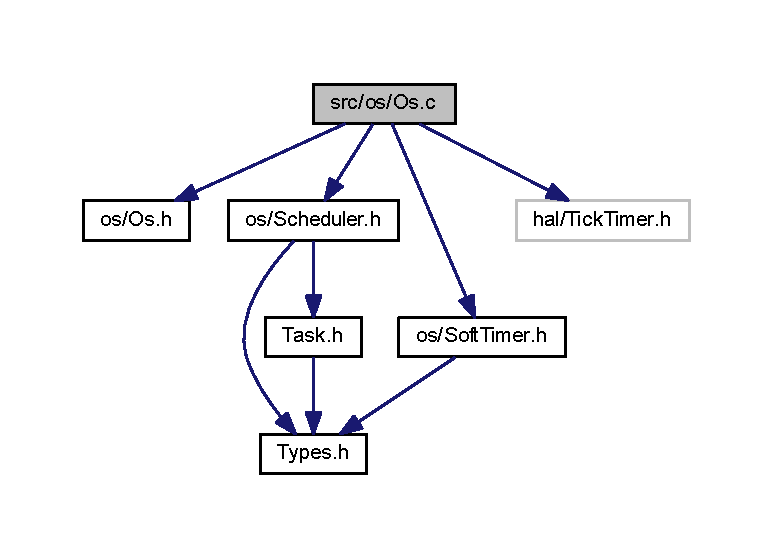
\includegraphics[width=350pt]{_os_8c__incl}
\end{center}
\end{figure}
\subsection*{Functions}
\begin{DoxyCompactItemize}
\item 
void \hyperlink{_os_8c_a9d68ac34142fe199f938dcdedd74318d}{O\+S\+\_\+init} (void)
\begin{DoxyCompactList}\small\item\em Initialize the O\+S. \end{DoxyCompactList}\end{DoxyCompactItemize}


\subsection{Detailed Description}
O\+S main module. 

\begin{DoxyVersion}{Version}
\$\+Id\+: \hyperlink{_os_8c}{Os.\+c} 281 2024-\/01-\/12 12\+:09\+:03\+Z leglaz \$ 
\end{DoxyVersion}


\subsection{Function Documentation}
\hypertarget{_os_8c_a9d68ac34142fe199f938dcdedd74318d}{\index{Os.\+c@{Os.\+c}!O\+S\+\_\+init@{O\+S\+\_\+init}}
\index{O\+S\+\_\+init@{O\+S\+\_\+init}!Os.\+c@{Os.\+c}}
\subsubsection[{O\+S\+\_\+init}]{\setlength{\rightskip}{0pt plus 5cm}void O\+S\+\_\+init (
\begin{DoxyParamCaption}
\item[{void}]{}
\end{DoxyParamCaption}
)}}\label{_os_8c_a9d68ac34142fe199f938dcdedd74318d}


Initialize the O\+S. 



References Scheduler\+\_\+init(), Soft\+Timer\+Handler\+\_\+init(), and Soft\+Timer\+Handler\+\_\+update().



Here is the call graph for this function\+:\nopagebreak
\begin{figure}[H]
\begin{center}
\leavevmode
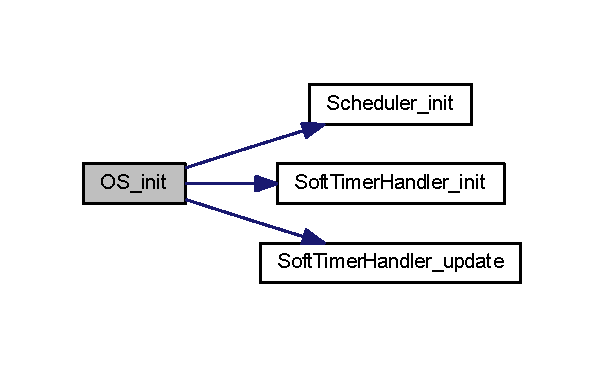
\includegraphics[width=290pt]{_os_8c_a9d68ac34142fe199f938dcdedd74318d_cgraph}
\end{center}
\end{figure}



\hypertarget{_os_8h}{\section{src/os/\+Os.h File Reference}
\label{_os_8h}\index{src/os/\+Os.\+h@{src/os/\+Os.\+h}}
}


Main header for O\+S module.  


This graph shows which files directly or indirectly include this file\+:\nopagebreak
\begin{figure}[H]
\begin{center}
\leavevmode
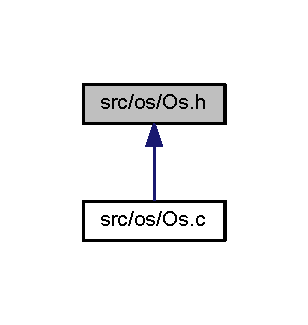
\includegraphics[width=148pt]{_os_8h__dep__incl}
\end{center}
\end{figure}
\subsection*{Functions}
\begin{DoxyCompactItemize}
\item 
void \hyperlink{_os_8h_a9d68ac34142fe199f938dcdedd74318d}{O\+S\+\_\+init} (void)
\begin{DoxyCompactList}\small\item\em Initialize the O\+S. \end{DoxyCompactList}\end{DoxyCompactItemize}


\subsection{Detailed Description}
Main header for O\+S module. 

\begin{DoxyVersion}{Version}
\$\+Id\+: \hyperlink{_os_8h}{Os.\+h} 294 2024-\/01-\/30 10\+:28\+:46\+Z leglaz \$ 
\end{DoxyVersion}


\subsection{Function Documentation}
\hypertarget{_os_8h_a9d68ac34142fe199f938dcdedd74318d}{\index{Os.\+h@{Os.\+h}!O\+S\+\_\+init@{O\+S\+\_\+init}}
\index{O\+S\+\_\+init@{O\+S\+\_\+init}!Os.\+h@{Os.\+h}}
\subsubsection[{O\+S\+\_\+init}]{\setlength{\rightskip}{0pt plus 5cm}void O\+S\+\_\+init (
\begin{DoxyParamCaption}
\item[{void}]{}
\end{DoxyParamCaption}
)}}\label{_os_8h_a9d68ac34142fe199f938dcdedd74318d}


Initialize the O\+S. 



References Scheduler\+\_\+init(), Soft\+Timer\+Handler\+\_\+init(), and Soft\+Timer\+Handler\+\_\+update().



Here is the call graph for this function\+:\nopagebreak
\begin{figure}[H]
\begin{center}
\leavevmode
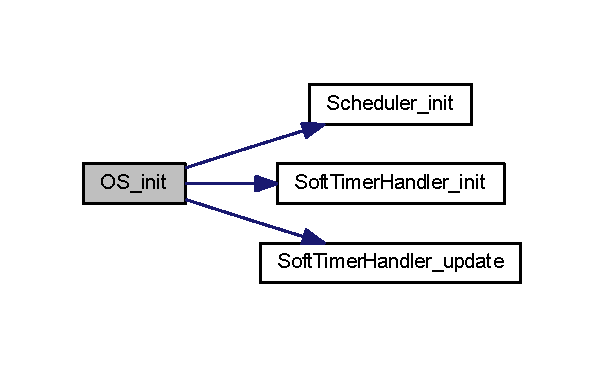
\includegraphics[width=290pt]{_os_8h_a9d68ac34142fe199f938dcdedd74318d_cgraph}
\end{center}
\end{figure}



\hypertarget{_scheduler_8c}{\section{src/os/\+Scheduler.c File Reference}
\label{_scheduler_8c}\index{src/os/\+Scheduler.\+c@{src/os/\+Scheduler.\+c}}
}


Simple task scheduler.  


{\ttfamily \#include \char`\"{}os/\+Scheduler.\+h\char`\"{}}\\*
{\ttfamily \#include \char`\"{}os/\+Task.\+h\char`\"{}}\\*
{\ttfamily \#include \char`\"{}hal/\+Irq.\+h\char`\"{}}\\*
Include dependency graph for Scheduler.\+c\+:\nopagebreak
\begin{figure}[H]
\begin{center}
\leavevmode
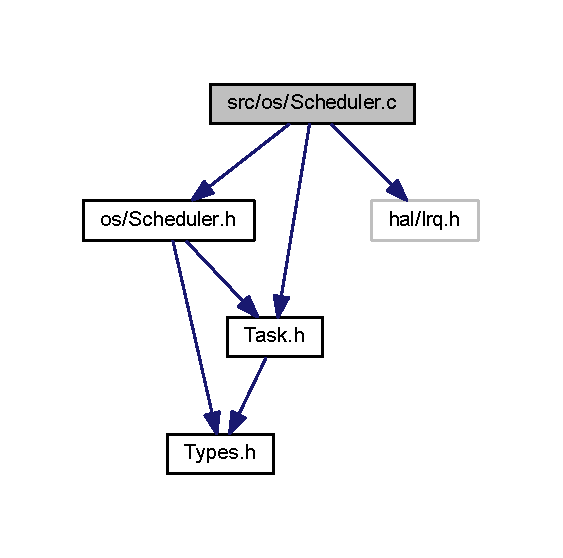
\includegraphics[width=270pt]{_scheduler_8c__incl}
\end{center}
\end{figure}
\subsection*{Functions}
\begin{DoxyCompactItemize}
\item 
\hypertarget{_scheduler_8c_a54f0b21668ad0d2c4d08e91a4a9577bf}{\hyperlink{_scheduler_8h_a4986e815f32ca6e968f160f11807f3b5}{Scheduler\+\_\+\+Ret} \hyperlink{_scheduler_8c_a54f0b21668ad0d2c4d08e91a4a9577bf}{Scheduler\+\_\+init} (void)}\label{_scheduler_8c_a54f0b21668ad0d2c4d08e91a4a9577bf}

\begin{DoxyCompactList}\small\item\em Initialize the scheduler module. \end{DoxyCompactList}\item 
void \hyperlink{_scheduler_8c_ac8b5914b94644528eb5212cded91576b}{Scheduler\+\_\+execute} (void)
\begin{DoxyCompactList}\small\item\em Execute one scheduler cycle. \end{DoxyCompactList}\item 
\hyperlink{_scheduler_8h_a4986e815f32ca6e968f160f11807f3b5}{Scheduler\+\_\+\+Ret} \hyperlink{_scheduler_8c_ab4e5be8ef348eae3a0ce316a8fe07bef}{Scheduler\+\_\+add\+Task} (\hyperlink{_task_8h_a77bbd51a2c7d34bd2aa764baadfb4b83}{Task} $\ast$p\+New\+Task)
\begin{DoxyCompactList}\small\item\em Add a task to the scheduler. \end{DoxyCompactList}\item 
\hyperlink{_scheduler_8h_a4986e815f32ca6e968f160f11807f3b5}{Scheduler\+\_\+\+Ret} \hyperlink{_scheduler_8c_af000216881be045d8a8d4b934c7caf67}{Scheduler\+\_\+remove\+Task} (\hyperlink{_task_8h_a77bbd51a2c7d34bd2aa764baadfb4b83}{Task} $\ast$p\+Task\+To\+Remove)
\begin{DoxyCompactList}\small\item\em Remove a task from the scheduler. \end{DoxyCompactList}\end{DoxyCompactItemize}


\subsection{Detailed Description}
Simple task scheduler. 

For a detailed description see the detailed description in \hyperlink{_scheduler_8h}{Scheduler.\+h}.

\begin{DoxyVersion}{Version}
\$\+Id\+: \hyperlink{_scheduler_8c}{Scheduler.\+c} 281 2024-\/01-\/12 12\+:09\+:03\+Z leglaz \$ 
\end{DoxyVersion}


\subsection{Function Documentation}
\hypertarget{_scheduler_8c_ab4e5be8ef348eae3a0ce316a8fe07bef}{\index{Scheduler.\+c@{Scheduler.\+c}!Scheduler\+\_\+add\+Task@{Scheduler\+\_\+add\+Task}}
\index{Scheduler\+\_\+add\+Task@{Scheduler\+\_\+add\+Task}!Scheduler.\+c@{Scheduler.\+c}}
\subsubsection[{Scheduler\+\_\+add\+Task}]{\setlength{\rightskip}{0pt plus 5cm}{\bf Scheduler\+\_\+\+Ret} Scheduler\+\_\+add\+Task (
\begin{DoxyParamCaption}
\item[{{\bf Task} $\ast$}]{task}
\end{DoxyParamCaption}
)}}\label{_scheduler_8c_ab4e5be8ef348eae3a0ce316a8fe07bef}


Add a task to the scheduler. 


\begin{DoxyParams}[1]{Parameters}
\mbox{\tt in}  & {\em task} & Pointer to task structure.\\
\hline
\end{DoxyParams}
\begin{DoxyReturn}{Returns}
true if successful, false if no more space or task already added. 
\end{DoxyReturn}


References N\+U\+L\+L, S\+C\+H\+E\+D\+U\+L\+E\+R\+\_\+\+M\+A\+X\+\_\+\+T\+A\+S\+K\+S, S\+C\+H\+E\+D\+U\+L\+E\+R\+\_\+\+R\+E\+T\+\_\+\+N\+O\+M\+O\+R\+E\+T\+A\+S\+K\+S, S\+C\+H\+E\+D\+U\+L\+E\+R\+\_\+\+R\+E\+T\+\_\+\+S\+U\+C\+C\+E\+S\+S, and S\+C\+H\+E\+D\+U\+L\+E\+R\+\_\+\+R\+E\+T\+\_\+\+T\+A\+S\+K\+A\+D\+D\+E\+D\+T\+W\+I\+C\+E.



Referenced by Main\+Task\+\_\+init().



Here is the caller graph for this function\+:\nopagebreak
\begin{figure}[H]
\begin{center}
\leavevmode
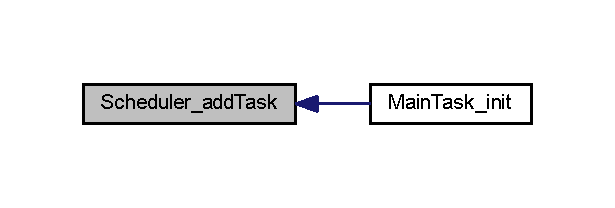
\includegraphics[width=295pt]{_scheduler_8c_ab4e5be8ef348eae3a0ce316a8fe07bef_icgraph}
\end{center}
\end{figure}


\hypertarget{_scheduler_8c_ac8b5914b94644528eb5212cded91576b}{\index{Scheduler.\+c@{Scheduler.\+c}!Scheduler\+\_\+execute@{Scheduler\+\_\+execute}}
\index{Scheduler\+\_\+execute@{Scheduler\+\_\+execute}!Scheduler.\+c@{Scheduler.\+c}}
\subsubsection[{Scheduler\+\_\+execute}]{\setlength{\rightskip}{0pt plus 5cm}void Scheduler\+\_\+execute (
\begin{DoxyParamCaption}
\item[{void}]{}
\end{DoxyParamCaption}
)}}\label{_scheduler_8c_ac8b5914b94644528eb5212cded91576b}


Execute one scheduler cycle. 

Call the work function of all running tasks sequentially. 

References N\+U\+L\+L, S\+C\+H\+E\+D\+U\+L\+E\+R\+\_\+\+M\+A\+X\+\_\+\+T\+A\+S\+K\+S, T\+A\+S\+K\+\_\+\+E\+X\+E\+C\+U\+T\+E, T\+A\+S\+K\+\_\+\+G\+E\+T\+\_\+\+S\+T\+A\+T\+E, and T\+A\+S\+K\+\_\+\+S\+T\+A\+T\+E\+\_\+\+R\+U\+N\+N\+I\+N\+G.

\hypertarget{_scheduler_8c_af000216881be045d8a8d4b934c7caf67}{\index{Scheduler.\+c@{Scheduler.\+c}!Scheduler\+\_\+remove\+Task@{Scheduler\+\_\+remove\+Task}}
\index{Scheduler\+\_\+remove\+Task@{Scheduler\+\_\+remove\+Task}!Scheduler.\+c@{Scheduler.\+c}}
\subsubsection[{Scheduler\+\_\+remove\+Task}]{\setlength{\rightskip}{0pt plus 5cm}{\bf Scheduler\+\_\+\+Ret} Scheduler\+\_\+remove\+Task (
\begin{DoxyParamCaption}
\item[{{\bf Task} $\ast$}]{task}
\end{DoxyParamCaption}
)}}\label{_scheduler_8c_af000216881be045d8a8d4b934c7caf67}


Remove a task from the scheduler. 


\begin{DoxyParams}[1]{Parameters}
\mbox{\tt in}  & {\em task} & Pointer to task structure.\\
\hline
\end{DoxyParams}
\begin{DoxyReturn}{Returns}
true if successful, falls if task not found. 
\end{DoxyReturn}


References N\+U\+L\+L, S\+C\+H\+E\+D\+U\+L\+E\+R\+\_\+\+M\+A\+X\+\_\+\+T\+A\+S\+K\+S, S\+C\+H\+E\+D\+U\+L\+E\+R\+\_\+\+R\+E\+T\+\_\+\+S\+U\+C\+C\+E\+S\+S, and S\+C\+H\+E\+D\+U\+L\+E\+R\+\_\+\+R\+E\+T\+\_\+\+U\+N\+K\+N\+O\+W\+N\+T\+A\+S\+K.


\hypertarget{_scheduler_8h}{\section{src/os/\+Scheduler.h File Reference}
\label{_scheduler_8h}\index{src/os/\+Scheduler.\+h@{src/os/\+Scheduler.\+h}}
}


Cooperative Round-\/\+Robin Scheduler.  


{\ttfamily \#include \char`\"{}Types.\+h\char`\"{}}\\*
{\ttfamily \#include \char`\"{}Task.\+h\char`\"{}}\\*
Include dependency graph for Scheduler.\+h\+:\nopagebreak
\begin{figure}[H]
\begin{center}
\leavevmode
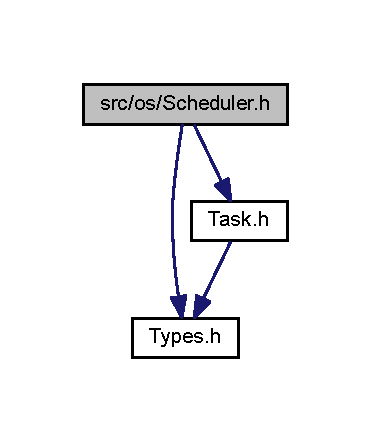
\includegraphics[width=178pt]{_scheduler_8h__incl}
\end{center}
\end{figure}
This graph shows which files directly or indirectly include this file\+:\nopagebreak
\begin{figure}[H]
\begin{center}
\leavevmode
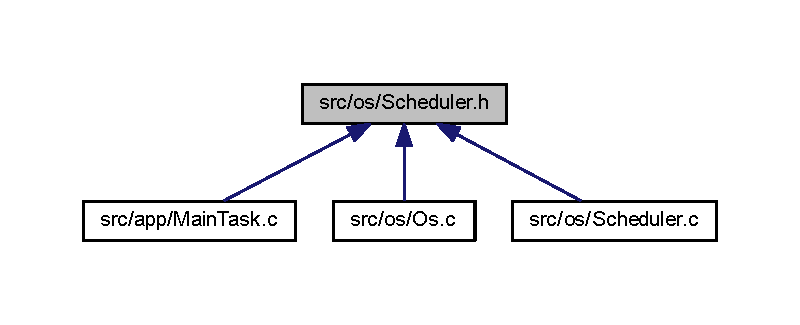
\includegraphics[width=350pt]{_scheduler_8h__dep__incl}
\end{center}
\end{figure}
\subsection*{Macros}
\begin{DoxyCompactItemize}
\item 
\#define \hyperlink{_scheduler_8h_af12cab9399b7b23dbe9fe6037e633cc8}{S\+C\+H\+E\+D\+U\+L\+E\+R\+\_\+\+M\+A\+X\+\_\+\+T\+A\+S\+K\+S}~(10)
\begin{DoxyCompactList}\small\item\em Maximum number of tasks that can be handled by the scheduler. \end{DoxyCompactList}\end{DoxyCompactItemize}
\subsection*{Enumerations}
\begin{DoxyCompactItemize}
\item 
enum \hyperlink{_scheduler_8h_a4986e815f32ca6e968f160f11807f3b5}{Scheduler\+\_\+\+Ret} \{ \\*
\hyperlink{_scheduler_8h_a4986e815f32ca6e968f160f11807f3b5a223c921c8a64ab80e8e2f086ae39037a}{S\+C\+H\+E\+D\+U\+L\+E\+R\+\_\+\+R\+E\+T\+\_\+\+S\+U\+C\+C\+E\+S\+S} = 0, 
\hyperlink{_scheduler_8h_a4986e815f32ca6e968f160f11807f3b5a722e14e81de2cd34ac141dd765b39fb4}{S\+C\+H\+E\+D\+U\+L\+E\+R\+\_\+\+R\+E\+T\+\_\+\+F\+A\+I\+L}, 
\hyperlink{_scheduler_8h_a4986e815f32ca6e968f160f11807f3b5a3ec86ed9827b2bb857f861b3dfb5cf5a}{S\+C\+H\+E\+D\+U\+L\+E\+R\+\_\+\+R\+E\+T\+\_\+\+N\+O\+M\+O\+R\+E\+T\+A\+S\+K\+S}, 
\hyperlink{_scheduler_8h_a4986e815f32ca6e968f160f11807f3b5a47071a842cf6ee2ec5e3165f70ef48c6}{S\+C\+H\+E\+D\+U\+L\+E\+R\+\_\+\+R\+E\+T\+\_\+\+T\+A\+S\+K\+A\+D\+D\+E\+D\+T\+W\+I\+C\+E}, 
\\*
\hyperlink{_scheduler_8h_a4986e815f32ca6e968f160f11807f3b5ad54312bce669278f7efec7ad9743e860}{S\+C\+H\+E\+D\+U\+L\+E\+R\+\_\+\+R\+E\+T\+\_\+\+U\+N\+K\+N\+O\+W\+N\+T\+A\+S\+K}
 \}
\begin{DoxyCompactList}\small\item\em Statuses of the scheduler. \end{DoxyCompactList}\end{DoxyCompactItemize}
\subsection*{Functions}
\begin{DoxyCompactItemize}
\item 
\hypertarget{_scheduler_8h_a54f0b21668ad0d2c4d08e91a4a9577bf}{\hyperlink{_scheduler_8h_a4986e815f32ca6e968f160f11807f3b5}{Scheduler\+\_\+\+Ret} \hyperlink{_scheduler_8h_a54f0b21668ad0d2c4d08e91a4a9577bf}{Scheduler\+\_\+init} (void)}\label{_scheduler_8h_a54f0b21668ad0d2c4d08e91a4a9577bf}

\begin{DoxyCompactList}\small\item\em Initialize the scheduler module. \end{DoxyCompactList}\item 
void \hyperlink{_scheduler_8h_ac8b5914b94644528eb5212cded91576b}{Scheduler\+\_\+execute} (void)
\begin{DoxyCompactList}\small\item\em Execute one scheduler cycle. \end{DoxyCompactList}\item 
\hyperlink{_scheduler_8h_a4986e815f32ca6e968f160f11807f3b5}{Scheduler\+\_\+\+Ret} \hyperlink{_scheduler_8h_a2010cdfa7c29f432542d6842f7e8d527}{Scheduler\+\_\+add\+Task} (\hyperlink{_task_8h_a77bbd51a2c7d34bd2aa764baadfb4b83}{Task} $\ast$task)
\begin{DoxyCompactList}\small\item\em Add a task to the scheduler. \end{DoxyCompactList}\item 
\hyperlink{_scheduler_8h_a4986e815f32ca6e968f160f11807f3b5}{Scheduler\+\_\+\+Ret} \hyperlink{_scheduler_8h_aa3171ba992feb30e29945f03da6a3a11}{Scheduler\+\_\+remove\+Task} (\hyperlink{_task_8h_a77bbd51a2c7d34bd2aa764baadfb4b83}{Task} $\ast$task)
\begin{DoxyCompactList}\small\item\em Remove a task from the scheduler. \end{DoxyCompactList}\end{DoxyCompactItemize}


\subsection{Detailed Description}
Cooperative Round-\/\+Robin Scheduler. 

A simple task scheduler that manages a fixed number of Tasks. Scheduling is cooperative, meaning task execution is done by calling a work cycle function that must return into the scheduler as fast as possible. Tasks in running state are called round-\/robion sequentially.

\begin{DoxyVersion}{Version}
\$\+Id\+: \hyperlink{_scheduler_8h}{Scheduler.\+h} 281 2024-\/01-\/12 12\+:09\+:03\+Z leglaz \$ 
\end{DoxyVersion}


\subsection{Macro Definition Documentation}
\hypertarget{_scheduler_8h_af12cab9399b7b23dbe9fe6037e633cc8}{\index{Scheduler.\+h@{Scheduler.\+h}!S\+C\+H\+E\+D\+U\+L\+E\+R\+\_\+\+M\+A\+X\+\_\+\+T\+A\+S\+K\+S@{S\+C\+H\+E\+D\+U\+L\+E\+R\+\_\+\+M\+A\+X\+\_\+\+T\+A\+S\+K\+S}}
\index{S\+C\+H\+E\+D\+U\+L\+E\+R\+\_\+\+M\+A\+X\+\_\+\+T\+A\+S\+K\+S@{S\+C\+H\+E\+D\+U\+L\+E\+R\+\_\+\+M\+A\+X\+\_\+\+T\+A\+S\+K\+S}!Scheduler.\+h@{Scheduler.\+h}}
\subsubsection[{S\+C\+H\+E\+D\+U\+L\+E\+R\+\_\+\+M\+A\+X\+\_\+\+T\+A\+S\+K\+S}]{\setlength{\rightskip}{0pt plus 5cm}\#define S\+C\+H\+E\+D\+U\+L\+E\+R\+\_\+\+M\+A\+X\+\_\+\+T\+A\+S\+K\+S~(10)}}\label{_scheduler_8h_af12cab9399b7b23dbe9fe6037e633cc8}


Maximum number of tasks that can be handled by the scheduler. 



Referenced by Scheduler\+\_\+add\+Task(), Scheduler\+\_\+execute(), Scheduler\+\_\+init(), and Scheduler\+\_\+remove\+Task().



\subsection{Enumeration Type Documentation}
\hypertarget{_scheduler_8h_a4986e815f32ca6e968f160f11807f3b5}{\index{Scheduler.\+h@{Scheduler.\+h}!Scheduler\+\_\+\+Ret@{Scheduler\+\_\+\+Ret}}
\index{Scheduler\+\_\+\+Ret@{Scheduler\+\_\+\+Ret}!Scheduler.\+h@{Scheduler.\+h}}
\subsubsection[{Scheduler\+\_\+\+Ret}]{\setlength{\rightskip}{0pt plus 5cm}enum {\bf Scheduler\+\_\+\+Ret}}}\label{_scheduler_8h_a4986e815f32ca6e968f160f11807f3b5}


Statuses of the scheduler. 

\begin{Desc}
\item[Enumerator]\par
\begin{description}
\index{S\+C\+H\+E\+D\+U\+L\+E\+R\+\_\+\+R\+E\+T\+\_\+\+S\+U\+C\+C\+E\+S\+S@{S\+C\+H\+E\+D\+U\+L\+E\+R\+\_\+\+R\+E\+T\+\_\+\+S\+U\+C\+C\+E\+S\+S}!Scheduler.\+h@{Scheduler.\+h}}\index{Scheduler.\+h@{Scheduler.\+h}!S\+C\+H\+E\+D\+U\+L\+E\+R\+\_\+\+R\+E\+T\+\_\+\+S\+U\+C\+C\+E\+S\+S@{S\+C\+H\+E\+D\+U\+L\+E\+R\+\_\+\+R\+E\+T\+\_\+\+S\+U\+C\+C\+E\+S\+S}}\item[{\em 
\hypertarget{_scheduler_8h_a4986e815f32ca6e968f160f11807f3b5a223c921c8a64ab80e8e2f086ae39037a}{S\+C\+H\+E\+D\+U\+L\+E\+R\+\_\+\+R\+E\+T\+\_\+\+S\+U\+C\+C\+E\+S\+S}\label{_scheduler_8h_a4986e815f32ca6e968f160f11807f3b5a223c921c8a64ab80e8e2f086ae39037a}
}]Operation succesful. \index{S\+C\+H\+E\+D\+U\+L\+E\+R\+\_\+\+R\+E\+T\+\_\+\+F\+A\+I\+L@{S\+C\+H\+E\+D\+U\+L\+E\+R\+\_\+\+R\+E\+T\+\_\+\+F\+A\+I\+L}!Scheduler.\+h@{Scheduler.\+h}}\index{Scheduler.\+h@{Scheduler.\+h}!S\+C\+H\+E\+D\+U\+L\+E\+R\+\_\+\+R\+E\+T\+\_\+\+F\+A\+I\+L@{S\+C\+H\+E\+D\+U\+L\+E\+R\+\_\+\+R\+E\+T\+\_\+\+F\+A\+I\+L}}\item[{\em 
\hypertarget{_scheduler_8h_a4986e815f32ca6e968f160f11807f3b5a722e14e81de2cd34ac141dd765b39fb4}{S\+C\+H\+E\+D\+U\+L\+E\+R\+\_\+\+R\+E\+T\+\_\+\+F\+A\+I\+L}\label{_scheduler_8h_a4986e815f32ca6e968f160f11807f3b5a722e14e81de2cd34ac141dd765b39fb4}
}]Operation failed. \index{S\+C\+H\+E\+D\+U\+L\+E\+R\+\_\+\+R\+E\+T\+\_\+\+N\+O\+M\+O\+R\+E\+T\+A\+S\+K\+S@{S\+C\+H\+E\+D\+U\+L\+E\+R\+\_\+\+R\+E\+T\+\_\+\+N\+O\+M\+O\+R\+E\+T\+A\+S\+K\+S}!Scheduler.\+h@{Scheduler.\+h}}\index{Scheduler.\+h@{Scheduler.\+h}!S\+C\+H\+E\+D\+U\+L\+E\+R\+\_\+\+R\+E\+T\+\_\+\+N\+O\+M\+O\+R\+E\+T\+A\+S\+K\+S@{S\+C\+H\+E\+D\+U\+L\+E\+R\+\_\+\+R\+E\+T\+\_\+\+N\+O\+M\+O\+R\+E\+T\+A\+S\+K\+S}}\item[{\em 
\hypertarget{_scheduler_8h_a4986e815f32ca6e968f160f11807f3b5a3ec86ed9827b2bb857f861b3dfb5cf5a}{S\+C\+H\+E\+D\+U\+L\+E\+R\+\_\+\+R\+E\+T\+\_\+\+N\+O\+M\+O\+R\+E\+T\+A\+S\+K\+S}\label{_scheduler_8h_a4986e815f32ca6e968f160f11807f3b5a3ec86ed9827b2bb857f861b3dfb5cf5a}
}]Maximum number of tasks reached. \index{S\+C\+H\+E\+D\+U\+L\+E\+R\+\_\+\+R\+E\+T\+\_\+\+T\+A\+S\+K\+A\+D\+D\+E\+D\+T\+W\+I\+C\+E@{S\+C\+H\+E\+D\+U\+L\+E\+R\+\_\+\+R\+E\+T\+\_\+\+T\+A\+S\+K\+A\+D\+D\+E\+D\+T\+W\+I\+C\+E}!Scheduler.\+h@{Scheduler.\+h}}\index{Scheduler.\+h@{Scheduler.\+h}!S\+C\+H\+E\+D\+U\+L\+E\+R\+\_\+\+R\+E\+T\+\_\+\+T\+A\+S\+K\+A\+D\+D\+E\+D\+T\+W\+I\+C\+E@{S\+C\+H\+E\+D\+U\+L\+E\+R\+\_\+\+R\+E\+T\+\_\+\+T\+A\+S\+K\+A\+D\+D\+E\+D\+T\+W\+I\+C\+E}}\item[{\em 
\hypertarget{_scheduler_8h_a4986e815f32ca6e968f160f11807f3b5a47071a842cf6ee2ec5e3165f70ef48c6}{S\+C\+H\+E\+D\+U\+L\+E\+R\+\_\+\+R\+E\+T\+\_\+\+T\+A\+S\+K\+A\+D\+D\+E\+D\+T\+W\+I\+C\+E}\label{_scheduler_8h_a4986e815f32ca6e968f160f11807f3b5a47071a842cf6ee2ec5e3165f70ef48c6}
}]Tried to add a task more then once. \index{S\+C\+H\+E\+D\+U\+L\+E\+R\+\_\+\+R\+E\+T\+\_\+\+U\+N\+K\+N\+O\+W\+N\+T\+A\+S\+K@{S\+C\+H\+E\+D\+U\+L\+E\+R\+\_\+\+R\+E\+T\+\_\+\+U\+N\+K\+N\+O\+W\+N\+T\+A\+S\+K}!Scheduler.\+h@{Scheduler.\+h}}\index{Scheduler.\+h@{Scheduler.\+h}!S\+C\+H\+E\+D\+U\+L\+E\+R\+\_\+\+R\+E\+T\+\_\+\+U\+N\+K\+N\+O\+W\+N\+T\+A\+S\+K@{S\+C\+H\+E\+D\+U\+L\+E\+R\+\_\+\+R\+E\+T\+\_\+\+U\+N\+K\+N\+O\+W\+N\+T\+A\+S\+K}}\item[{\em 
\hypertarget{_scheduler_8h_a4986e815f32ca6e968f160f11807f3b5ad54312bce669278f7efec7ad9743e860}{S\+C\+H\+E\+D\+U\+L\+E\+R\+\_\+\+R\+E\+T\+\_\+\+U\+N\+K\+N\+O\+W\+N\+T\+A\+S\+K}\label{_scheduler_8h_a4986e815f32ca6e968f160f11807f3b5ad54312bce669278f7efec7ad9743e860}
}]Task was not added. \end{description}
\end{Desc}


\subsection{Function Documentation}
\hypertarget{_scheduler_8h_a2010cdfa7c29f432542d6842f7e8d527}{\index{Scheduler.\+h@{Scheduler.\+h}!Scheduler\+\_\+add\+Task@{Scheduler\+\_\+add\+Task}}
\index{Scheduler\+\_\+add\+Task@{Scheduler\+\_\+add\+Task}!Scheduler.\+h@{Scheduler.\+h}}
\subsubsection[{Scheduler\+\_\+add\+Task}]{\setlength{\rightskip}{0pt plus 5cm}{\bf Scheduler\+\_\+\+Ret} Scheduler\+\_\+add\+Task (
\begin{DoxyParamCaption}
\item[{{\bf Task} $\ast$}]{task}
\end{DoxyParamCaption}
)}}\label{_scheduler_8h_a2010cdfa7c29f432542d6842f7e8d527}


Add a task to the scheduler. 


\begin{DoxyParams}[1]{Parameters}
\mbox{\tt in}  & {\em task} & Pointer to task structure.\\
\hline
\end{DoxyParams}
\begin{DoxyReturn}{Returns}
true if successful, false if no more space or task already added. 
\end{DoxyReturn}


References N\+U\+L\+L, S\+C\+H\+E\+D\+U\+L\+E\+R\+\_\+\+M\+A\+X\+\_\+\+T\+A\+S\+K\+S, S\+C\+H\+E\+D\+U\+L\+E\+R\+\_\+\+R\+E\+T\+\_\+\+N\+O\+M\+O\+R\+E\+T\+A\+S\+K\+S, S\+C\+H\+E\+D\+U\+L\+E\+R\+\_\+\+R\+E\+T\+\_\+\+S\+U\+C\+C\+E\+S\+S, and S\+C\+H\+E\+D\+U\+L\+E\+R\+\_\+\+R\+E\+T\+\_\+\+T\+A\+S\+K\+A\+D\+D\+E\+D\+T\+W\+I\+C\+E.



Referenced by Main\+Task\+\_\+init().



Here is the caller graph for this function\+:\nopagebreak
\begin{figure}[H]
\begin{center}
\leavevmode
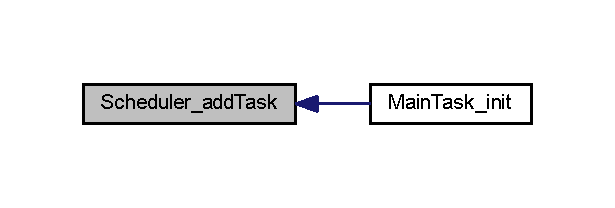
\includegraphics[width=295pt]{_scheduler_8h_a2010cdfa7c29f432542d6842f7e8d527_icgraph}
\end{center}
\end{figure}


\hypertarget{_scheduler_8h_ac8b5914b94644528eb5212cded91576b}{\index{Scheduler.\+h@{Scheduler.\+h}!Scheduler\+\_\+execute@{Scheduler\+\_\+execute}}
\index{Scheduler\+\_\+execute@{Scheduler\+\_\+execute}!Scheduler.\+h@{Scheduler.\+h}}
\subsubsection[{Scheduler\+\_\+execute}]{\setlength{\rightskip}{0pt plus 5cm}void Scheduler\+\_\+execute (
\begin{DoxyParamCaption}
\item[{void}]{}
\end{DoxyParamCaption}
)}}\label{_scheduler_8h_ac8b5914b94644528eb5212cded91576b}


Execute one scheduler cycle. 

Call the work function of all running tasks sequentially. 

References N\+U\+L\+L, S\+C\+H\+E\+D\+U\+L\+E\+R\+\_\+\+M\+A\+X\+\_\+\+T\+A\+S\+K\+S, T\+A\+S\+K\+\_\+\+E\+X\+E\+C\+U\+T\+E, T\+A\+S\+K\+\_\+\+G\+E\+T\+\_\+\+S\+T\+A\+T\+E, and T\+A\+S\+K\+\_\+\+S\+T\+A\+T\+E\+\_\+\+R\+U\+N\+N\+I\+N\+G.

\hypertarget{_scheduler_8h_aa3171ba992feb30e29945f03da6a3a11}{\index{Scheduler.\+h@{Scheduler.\+h}!Scheduler\+\_\+remove\+Task@{Scheduler\+\_\+remove\+Task}}
\index{Scheduler\+\_\+remove\+Task@{Scheduler\+\_\+remove\+Task}!Scheduler.\+h@{Scheduler.\+h}}
\subsubsection[{Scheduler\+\_\+remove\+Task}]{\setlength{\rightskip}{0pt plus 5cm}{\bf Scheduler\+\_\+\+Ret} Scheduler\+\_\+remove\+Task (
\begin{DoxyParamCaption}
\item[{{\bf Task} $\ast$}]{task}
\end{DoxyParamCaption}
)}}\label{_scheduler_8h_aa3171ba992feb30e29945f03da6a3a11}


Remove a task from the scheduler. 


\begin{DoxyParams}[1]{Parameters}
\mbox{\tt in}  & {\em task} & Pointer to task structure.\\
\hline
\end{DoxyParams}
\begin{DoxyReturn}{Returns}
true if successful, falls if task not found. 
\end{DoxyReturn}


References N\+U\+L\+L, S\+C\+H\+E\+D\+U\+L\+E\+R\+\_\+\+M\+A\+X\+\_\+\+T\+A\+S\+K\+S, S\+C\+H\+E\+D\+U\+L\+E\+R\+\_\+\+R\+E\+T\+\_\+\+S\+U\+C\+C\+E\+S\+S, and S\+C\+H\+E\+D\+U\+L\+E\+R\+\_\+\+R\+E\+T\+\_\+\+U\+N\+K\+N\+O\+W\+N\+T\+A\+S\+K.


\hypertarget{_soft_timer_8c}{\section{src/os/\+Soft\+Timer.c File Reference}
\label{_soft_timer_8c}\index{src/os/\+Soft\+Timer.\+c@{src/os/\+Soft\+Timer.\+c}}
}


Soft\+Timer implementation.  


{\ttfamily \#include \char`\"{}os/\+Soft\+Timer.\+h\char`\"{}}\\*
{\ttfamily \#include \char`\"{}hal/\+Tick\+Timer.\+h\char`\"{}}\\*
{\ttfamily \#include $<$util/atomic.\+h$>$}\\*
Include dependency graph for Soft\+Timer.\+c\+:\nopagebreak
\begin{figure}[H]
\begin{center}
\leavevmode
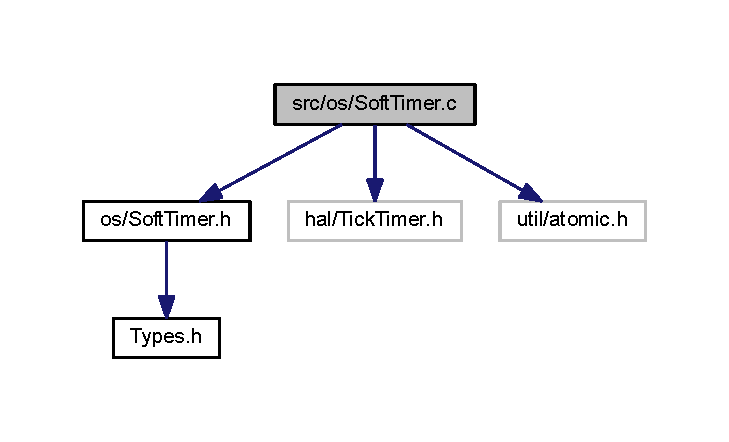
\includegraphics[width=350pt]{_soft_timer_8c__incl}
\end{center}
\end{figure}
\subsection*{Macros}
\begin{DoxyCompactItemize}
\item 
\hypertarget{_soft_timer_8c_ad8306d5e8474f678cee4b263f8358591}{\#define \hyperlink{_soft_timer_8c_ad8306d5e8474f678cee4b263f8358591}{S\+O\+F\+T\+\_\+\+T\+I\+M\+E\+R\+\_\+\+M\+A\+X\+\_\+\+T\+I\+M\+E\+R}~(10u)}\label{_soft_timer_8c_ad8306d5e8474f678cee4b263f8358591}

\begin{DoxyCompactList}\small\item\em Maximum number of soft timers. \end{DoxyCompactList}\end{DoxyCompactItemize}
\subsection*{Functions}
\begin{DoxyCompactItemize}
\item 
void \hyperlink{_soft_timer_8c_a7dc718cbe43429746a7bb831c867fbdc}{Soft\+Timer\+\_\+init} (\hyperlink{_soft_timer_8h_a5e4ffe7f5109549a43b9971bafa8f614}{Soft\+Timer} $\ast$p\+Soft\+Timer)
\begin{DoxyCompactList}\small\item\em Initialize a soft timer structure. \end{DoxyCompactList}\item 
\hyperlink{_soft_timer_8h_a58342871750337e1b043e19e4e565204}{Soft\+Timer\+\_\+\+Ret} \hyperlink{_soft_timer_8c_afa63b52bac28804a7a67a0aaebf1c182}{Soft\+Timer\+\_\+start} (\hyperlink{_soft_timer_8h_a5e4ffe7f5109549a43b9971bafa8f614}{Soft\+Timer} $\ast$p\+Soft\+Timer, \hyperlink{_types_8h_aad0fc9943ec46ed9388d30c8ebe52b77}{U\+Int16} thres\+Hold)
\begin{DoxyCompactList}\small\item\em Start a soft timer with a countdown value. \end{DoxyCompactList}\item 
\hyperlink{_soft_timer_8h_a58342871750337e1b043e19e4e565204}{Soft\+Timer\+\_\+\+Ret} \hyperlink{_soft_timer_8c_a9169331d10ecae626b4884804df30b61}{Soft\+Timer\+\_\+\+Stop} (\hyperlink{_soft_timer_8h_a5e4ffe7f5109549a43b9971bafa8f614}{Soft\+Timer} $\ast$p\+Soft\+Timer)
\begin{DoxyCompactList}\small\item\em Update a soft timer (interrupt context!). \end{DoxyCompactList}\item 
void \hyperlink{_soft_timer_8c_a43d0fbf6361bd5b7d5d67bc8879f068d}{Soft\+Timer\+\_\+\+Update} (\hyperlink{_soft_timer_8h_a5e4ffe7f5109549a43b9971bafa8f614}{Soft\+Timer} $\ast$p\+Soft\+Timer)
\begin{DoxyCompactList}\small\item\em Update a soft timer (interrupt context!). \end{DoxyCompactList}\item 
\hyperlink{_soft_timer_8h_a58342871750337e1b043e19e4e565204}{Soft\+Timer\+\_\+\+Ret} \hyperlink{_soft_timer_8c_af65202ec6e69ab0744e2a942b001419c}{Soft\+Timer\+\_\+restart} (\hyperlink{_soft_timer_8h_a5e4ffe7f5109549a43b9971bafa8f614}{Soft\+Timer} $\ast$p\+Soft\+Timer)
\begin{DoxyCompactList}\small\item\em Update a soft timer with thresh\+Hold from former start call. \end{DoxyCompactList}\item 
\hyperlink{_types_8h_aad0fc9943ec46ed9388d30c8ebe52b77}{U\+Int16} \hyperlink{_soft_timer_8c_a3ebeed43ab2994f280616c02f0232a79}{Soft\+Timer\+\_\+get} (\hyperlink{_soft_timer_8h_a5e4ffe7f5109549a43b9971bafa8f614}{Soft\+Timer} $\ast$p\+Soft\+Timer)
\begin{DoxyCompactList}\small\item\em Get current countdown value of a soft timer. \end{DoxyCompactList}\item 
\hypertarget{_soft_timer_8c_a66e135f2168b6d86cb842fad599dd139}{void \hyperlink{_soft_timer_8c_a66e135f2168b6d86cb842fad599dd139}{Soft\+Timer\+Handler\+\_\+init} ()}\label{_soft_timer_8c_a66e135f2168b6d86cb842fad599dd139}

\begin{DoxyCompactList}\small\item\em Initialize the soft timer handler. \end{DoxyCompactList}\item 
\hyperlink{_soft_timer_8h_a58342871750337e1b043e19e4e565204}{Soft\+Timer\+\_\+\+Ret} \hyperlink{_soft_timer_8c_a613921965e70da83d217293c54c5fb2f}{Soft\+Timer\+Handler\+\_\+register} (\hyperlink{_soft_timer_8h_a5e4ffe7f5109549a43b9971bafa8f614}{Soft\+Timer} $\ast$p\+New\+Soft\+Timer)
\begin{DoxyCompactList}\small\item\em Register a soft timer with the handler. \end{DoxyCompactList}\item 
\hyperlink{_soft_timer_8h_a58342871750337e1b043e19e4e565204}{Soft\+Timer\+\_\+\+Ret} \hyperlink{_soft_timer_8c_a3a1035d1c666892fc49a51e85c748fa3}{Soft\+Timer\+Handler\+\_\+un\+Register} (\hyperlink{_soft_timer_8h_a5e4ffe7f5109549a43b9971bafa8f614}{Soft\+Timer} $\ast$p\+Soft\+Timer\+To\+Remove)
\begin{DoxyCompactList}\small\item\em De-\/\+Register a soft timer from the handler. \end{DoxyCompactList}\item 
void \hyperlink{_soft_timer_8c_a158d51a820ff74bc56473d9f695f2531}{Soft\+Timer\+Handler\+\_\+update} ()
\begin{DoxyCompactList}\small\item\em Update all registered soft timer (interrupt context!). \end{DoxyCompactList}\item 
\hyperlink{_types_8h_aa1d7d331b6d522d6d9840fece27108d8}{U\+Int64} \hyperlink{_soft_timer_8c_abc0b5659889d661d7deb93e8dd4c9136}{Soft\+Timer\+\_\+get\+Timestamp\+Ms} ()
\begin{DoxyCompactList}\small\item\em Get the current value of the tick Counter in micro seconds since startup. \end{DoxyCompactList}\end{DoxyCompactItemize}


\subsection{Detailed Description}
Soft\+Timer implementation. 

For a detailed description see the detailed description in \hyperlink{_soft_timer_8h}{Soft\+Timer.\+h}.

\begin{DoxyVersion}{Version}
\$\+Id\+: \hyperlink{_soft_timer_8c}{Soft\+Timer.\+c} 281 2024-\/01-\/12 12\+:09\+:03\+Z leglaz \$ 
\end{DoxyVersion}


\subsection{Function Documentation}
\hypertarget{_soft_timer_8c_a3ebeed43ab2994f280616c02f0232a79}{\index{Soft\+Timer.\+c@{Soft\+Timer.\+c}!Soft\+Timer\+\_\+get@{Soft\+Timer\+\_\+get}}
\index{Soft\+Timer\+\_\+get@{Soft\+Timer\+\_\+get}!Soft\+Timer.\+c@{Soft\+Timer.\+c}}
\subsubsection[{Soft\+Timer\+\_\+get}]{\setlength{\rightskip}{0pt plus 5cm}{\bf U\+Int16} Soft\+Timer\+\_\+get (
\begin{DoxyParamCaption}
\item[{{\bf Soft\+Timer} $\ast$}]{p\+Soft\+Timer}
\end{DoxyParamCaption}
)}}\label{_soft_timer_8c_a3ebeed43ab2994f280616c02f0232a79}


Get current countdown value of a soft timer. 


\begin{DoxyParams}[1]{Parameters}
\mbox{\tt in}  & {\em p\+Soft\+Timer} & A soft timer structure. \\
\hline
\end{DoxyParams}


References tag\+\_\+\+Soft\+Timer\+::counter.

\hypertarget{_soft_timer_8c_abc0b5659889d661d7deb93e8dd4c9136}{\index{Soft\+Timer.\+c@{Soft\+Timer.\+c}!Soft\+Timer\+\_\+get\+Timestamp\+Ms@{Soft\+Timer\+\_\+get\+Timestamp\+Ms}}
\index{Soft\+Timer\+\_\+get\+Timestamp\+Ms@{Soft\+Timer\+\_\+get\+Timestamp\+Ms}!Soft\+Timer.\+c@{Soft\+Timer.\+c}}
\subsubsection[{Soft\+Timer\+\_\+get\+Timestamp\+Ms}]{\setlength{\rightskip}{0pt plus 5cm}{\bf U\+Int64} Soft\+Timer\+\_\+get\+Timestamp\+Ms (
\begin{DoxyParamCaption}
\item[{void}]{}
\end{DoxyParamCaption}
)}}\label{_soft_timer_8c_abc0b5659889d661d7deb93e8dd4c9136}


Get the current value of the tick Counter in micro seconds since startup. 

\begin{DoxyReturn}{Returns}
tick counter value in microseconds. 
\end{DoxyReturn}
\hypertarget{_soft_timer_8c_a7dc718cbe43429746a7bb831c867fbdc}{\index{Soft\+Timer.\+c@{Soft\+Timer.\+c}!Soft\+Timer\+\_\+init@{Soft\+Timer\+\_\+init}}
\index{Soft\+Timer\+\_\+init@{Soft\+Timer\+\_\+init}!Soft\+Timer.\+c@{Soft\+Timer.\+c}}
\subsubsection[{Soft\+Timer\+\_\+init}]{\setlength{\rightskip}{0pt plus 5cm}void Soft\+Timer\+\_\+init (
\begin{DoxyParamCaption}
\item[{{\bf Soft\+Timer} $\ast$}]{p\+Soft\+Timer}
\end{DoxyParamCaption}
)}}\label{_soft_timer_8c_a7dc718cbe43429746a7bb831c867fbdc}


Initialize a soft timer structure. 


\begin{DoxyParams}[1]{Parameters}
\mbox{\tt in}  & {\em p\+Soft\+Timer} & A soft timer structure. \\
\hline
\end{DoxyParams}


References tag\+\_\+\+Soft\+Timer\+::counter, S\+O\+F\+T\+\_\+\+T\+I\+M\+E\+R\+\_\+\+U\+N\+R\+E\+G\+I\+S\+T\+E\+R\+E\+D, tag\+\_\+\+Soft\+Timer\+::state, and tag\+\_\+\+Soft\+Timer\+::thresh\+Hold.

\hypertarget{_soft_timer_8c_af65202ec6e69ab0744e2a942b001419c}{\index{Soft\+Timer.\+c@{Soft\+Timer.\+c}!Soft\+Timer\+\_\+restart@{Soft\+Timer\+\_\+restart}}
\index{Soft\+Timer\+\_\+restart@{Soft\+Timer\+\_\+restart}!Soft\+Timer.\+c@{Soft\+Timer.\+c}}
\subsubsection[{Soft\+Timer\+\_\+restart}]{\setlength{\rightskip}{0pt plus 5cm}{\bf Soft\+Timer\+\_\+\+Ret} Soft\+Timer\+\_\+restart (
\begin{DoxyParamCaption}
\item[{{\bf Soft\+Timer} $\ast$}]{p\+Soft\+Timer}
\end{DoxyParamCaption}
)}}\label{_soft_timer_8c_af65202ec6e69ab0744e2a942b001419c}


Update a soft timer with thresh\+Hold from former start call. 


\begin{DoxyParams}[1]{Parameters}
\mbox{\tt in}  & {\em p\+Soft\+Timer} & A soft timer structure. \\
\hline
\end{DoxyParams}


References Soft\+Timer\+\_\+start(), and tag\+\_\+\+Soft\+Timer\+::thresh\+Hold.



Here is the call graph for this function\+:\nopagebreak
\begin{figure}[H]
\begin{center}
\leavevmode
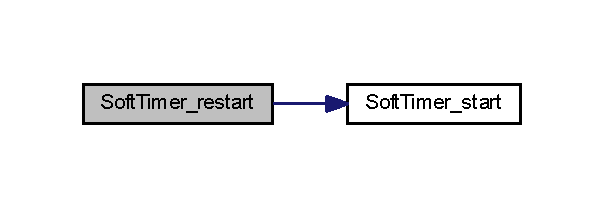
\includegraphics[width=290pt]{_soft_timer_8c_af65202ec6e69ab0744e2a942b001419c_cgraph}
\end{center}
\end{figure}


\hypertarget{_soft_timer_8c_afa63b52bac28804a7a67a0aaebf1c182}{\index{Soft\+Timer.\+c@{Soft\+Timer.\+c}!Soft\+Timer\+\_\+start@{Soft\+Timer\+\_\+start}}
\index{Soft\+Timer\+\_\+start@{Soft\+Timer\+\_\+start}!Soft\+Timer.\+c@{Soft\+Timer.\+c}}
\subsubsection[{Soft\+Timer\+\_\+start}]{\setlength{\rightskip}{0pt plus 5cm}{\bf Soft\+Timer\+\_\+\+Ret} Soft\+Timer\+\_\+start (
\begin{DoxyParamCaption}
\item[{{\bf Soft\+Timer} $\ast$}]{p\+Soft\+Timer, }
\item[{{\bf U\+Int16}}]{thres\+Hold}
\end{DoxyParamCaption}
)}}\label{_soft_timer_8c_afa63b52bac28804a7a67a0aaebf1c182}


Start a soft timer with a countdown value. 


\begin{DoxyParams}[1]{Parameters}
\mbox{\tt in}  & {\em p\+Soft\+Timer} & A soft timer structure. \\
\hline
\mbox{\tt in}  & {\em thres\+Hold} & The start value of the count down. \\
\hline
\end{DoxyParams}


References tag\+\_\+\+Soft\+Timer\+::counter, S\+O\+F\+T\+\_\+\+T\+I\+M\+E\+R\+\_\+\+R\+U\+N\+N\+I\+N\+G, S\+O\+F\+T\+\_\+\+T\+I\+M\+E\+R\+\_\+\+U\+N\+R\+E\+G\+I\+S\+T\+E\+R\+E\+D, S\+O\+F\+T\+T\+I\+M\+E\+R\+\_\+\+R\+E\+T\+\_\+\+N\+O\+T\+R\+E\+G\+I\+S\+T\+E\+R\+E\+D, S\+O\+F\+T\+T\+I\+M\+E\+R\+\_\+\+R\+E\+T\+\_\+\+S\+U\+C\+C\+E\+S\+S, tag\+\_\+\+Soft\+Timer\+::state, and tag\+\_\+\+Soft\+Timer\+::thresh\+Hold.



Referenced by Soft\+Timer\+\_\+restart().



Here is the caller graph for this function\+:\nopagebreak
\begin{figure}[H]
\begin{center}
\leavevmode
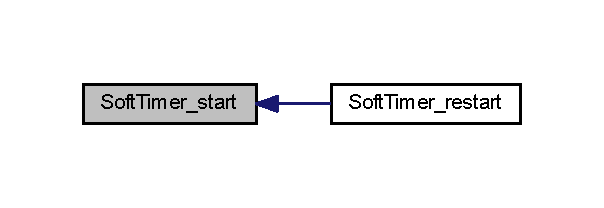
\includegraphics[width=290pt]{_soft_timer_8c_afa63b52bac28804a7a67a0aaebf1c182_icgraph}
\end{center}
\end{figure}


\hypertarget{_soft_timer_8c_a9169331d10ecae626b4884804df30b61}{\index{Soft\+Timer.\+c@{Soft\+Timer.\+c}!Soft\+Timer\+\_\+\+Stop@{Soft\+Timer\+\_\+\+Stop}}
\index{Soft\+Timer\+\_\+\+Stop@{Soft\+Timer\+\_\+\+Stop}!Soft\+Timer.\+c@{Soft\+Timer.\+c}}
\subsubsection[{Soft\+Timer\+\_\+\+Stop}]{\setlength{\rightskip}{0pt plus 5cm}{\bf Soft\+Timer\+\_\+\+Ret} Soft\+Timer\+\_\+\+Stop (
\begin{DoxyParamCaption}
\item[{{\bf Soft\+Timer} $\ast$}]{p\+Soft\+Timer}
\end{DoxyParamCaption}
)}}\label{_soft_timer_8c_a9169331d10ecae626b4884804df30b61}


Update a soft timer (interrupt context!). 


\begin{DoxyParams}[1]{Parameters}
\mbox{\tt in}  & {\em p\+Soft\+Timer} & A soft timer structure. \\
\hline
\end{DoxyParams}


References S\+O\+F\+T\+\_\+\+T\+I\+M\+E\+R\+\_\+\+S\+T\+O\+P\+P\+E\+D, S\+O\+F\+T\+\_\+\+T\+I\+M\+E\+R\+\_\+\+U\+N\+R\+E\+G\+I\+S\+T\+E\+R\+E\+D, S\+O\+F\+T\+T\+I\+M\+E\+R\+\_\+\+R\+E\+T\+\_\+\+N\+O\+T\+R\+E\+G\+I\+S\+T\+E\+R\+E\+D, S\+O\+F\+T\+T\+I\+M\+E\+R\+\_\+\+R\+E\+T\+\_\+\+S\+U\+C\+C\+E\+S\+S, and tag\+\_\+\+Soft\+Timer\+::state.

\hypertarget{_soft_timer_8c_a43d0fbf6361bd5b7d5d67bc8879f068d}{\index{Soft\+Timer.\+c@{Soft\+Timer.\+c}!Soft\+Timer\+\_\+\+Update@{Soft\+Timer\+\_\+\+Update}}
\index{Soft\+Timer\+\_\+\+Update@{Soft\+Timer\+\_\+\+Update}!Soft\+Timer.\+c@{Soft\+Timer.\+c}}
\subsubsection[{Soft\+Timer\+\_\+\+Update}]{\setlength{\rightskip}{0pt plus 5cm}void Soft\+Timer\+\_\+\+Update (
\begin{DoxyParamCaption}
\item[{{\bf Soft\+Timer} $\ast$}]{p\+Soft\+Timer}
\end{DoxyParamCaption}
)}}\label{_soft_timer_8c_a43d0fbf6361bd5b7d5d67bc8879f068d}


Update a soft timer (interrupt context!). 


\begin{DoxyParams}[1]{Parameters}
\mbox{\tt in}  & {\em p\+Soft\+Timer} & A soft timer structure. \\
\hline
\end{DoxyParams}


References tag\+\_\+\+Soft\+Timer\+::counter, S\+O\+F\+T\+\_\+\+T\+I\+M\+E\+R\+\_\+\+R\+U\+N\+N\+I\+N\+G, and tag\+\_\+\+Soft\+Timer\+::state.

\hypertarget{_soft_timer_8c_a613921965e70da83d217293c54c5fb2f}{\index{Soft\+Timer.\+c@{Soft\+Timer.\+c}!Soft\+Timer\+Handler\+\_\+register@{Soft\+Timer\+Handler\+\_\+register}}
\index{Soft\+Timer\+Handler\+\_\+register@{Soft\+Timer\+Handler\+\_\+register}!Soft\+Timer.\+c@{Soft\+Timer.\+c}}
\subsubsection[{Soft\+Timer\+Handler\+\_\+register}]{\setlength{\rightskip}{0pt plus 5cm}{\bf Soft\+Timer\+\_\+\+Ret} Soft\+Timer\+Handler\+\_\+register (
\begin{DoxyParamCaption}
\item[{{\bf Soft\+Timer} $\ast$}]{p\+Soft\+Timer}
\end{DoxyParamCaption}
)}}\label{_soft_timer_8c_a613921965e70da83d217293c54c5fb2f}


Register a soft timer with the handler. 


\begin{DoxyParams}[1]{Parameters}
\mbox{\tt in}  & {\em p\+Soft\+Timer} & A soft timer structure. \\
\hline
\end{DoxyParams}


References N\+U\+L\+L, S\+O\+F\+T\+\_\+\+T\+I\+M\+E\+R\+\_\+\+M\+A\+X\+\_\+\+T\+I\+M\+E\+R, S\+O\+F\+T\+\_\+\+T\+I\+M\+E\+R\+\_\+\+S\+T\+O\+P\+P\+E\+D, S\+O\+F\+T\+T\+I\+M\+E\+R\+\_\+\+R\+E\+T\+\_\+\+A\+L\+R\+E\+A\+D\+Y\+R\+E\+G\+I\+S\+T\+E\+R\+E\+D, S\+O\+F\+T\+T\+I\+M\+E\+R\+\_\+\+R\+E\+T\+\_\+\+N\+O\+M\+O\+R\+E\+T\+I\+M\+E\+R\+S, S\+O\+F\+T\+T\+I\+M\+E\+R\+\_\+\+R\+E\+T\+\_\+\+S\+U\+C\+C\+E\+S\+S, and tag\+\_\+\+Soft\+Timer\+::state.

\hypertarget{_soft_timer_8c_a3a1035d1c666892fc49a51e85c748fa3}{\index{Soft\+Timer.\+c@{Soft\+Timer.\+c}!Soft\+Timer\+Handler\+\_\+un\+Register@{Soft\+Timer\+Handler\+\_\+un\+Register}}
\index{Soft\+Timer\+Handler\+\_\+un\+Register@{Soft\+Timer\+Handler\+\_\+un\+Register}!Soft\+Timer.\+c@{Soft\+Timer.\+c}}
\subsubsection[{Soft\+Timer\+Handler\+\_\+un\+Register}]{\setlength{\rightskip}{0pt plus 5cm}{\bf Soft\+Timer\+\_\+\+Ret} Soft\+Timer\+Handler\+\_\+un\+Register (
\begin{DoxyParamCaption}
\item[{{\bf Soft\+Timer} $\ast$}]{p\+Soft\+Timer}
\end{DoxyParamCaption}
)}}\label{_soft_timer_8c_a3a1035d1c666892fc49a51e85c748fa3}


De-\/\+Register a soft timer from the handler. 


\begin{DoxyParams}[1]{Parameters}
\mbox{\tt in}  & {\em p\+Soft\+Timer} & A soft timer structure. \\
\hline
\end{DoxyParams}


References N\+U\+L\+L, S\+O\+F\+T\+\_\+\+T\+I\+M\+E\+R\+\_\+\+M\+A\+X\+\_\+\+T\+I\+M\+E\+R, S\+O\+F\+T\+T\+I\+M\+E\+R\+\_\+\+R\+E\+T\+\_\+\+S\+U\+C\+C\+E\+S\+S, and S\+O\+F\+T\+T\+I\+M\+E\+R\+\_\+\+R\+E\+T\+\_\+\+U\+N\+K\+N\+O\+W\+N\+T\+I\+M\+E\+R.

\hypertarget{_soft_timer_8c_a158d51a820ff74bc56473d9f695f2531}{\index{Soft\+Timer.\+c@{Soft\+Timer.\+c}!Soft\+Timer\+Handler\+\_\+update@{Soft\+Timer\+Handler\+\_\+update}}
\index{Soft\+Timer\+Handler\+\_\+update@{Soft\+Timer\+Handler\+\_\+update}!Soft\+Timer.\+c@{Soft\+Timer.\+c}}
\subsubsection[{Soft\+Timer\+Handler\+\_\+update}]{\setlength{\rightskip}{0pt plus 5cm}void Soft\+Timer\+Handler\+\_\+update (
\begin{DoxyParamCaption}
\item[{void}]{}
\end{DoxyParamCaption}
)}}\label{_soft_timer_8c_a158d51a820ff74bc56473d9f695f2531}


Update all registered soft timer (interrupt context!). 



References tag\+\_\+\+Soft\+Timer\+::counter, N\+U\+L\+L, S\+O\+F\+T\+\_\+\+T\+I\+M\+E\+R\+\_\+\+M\+A\+X\+\_\+\+T\+I\+M\+E\+R, S\+O\+F\+T\+\_\+\+T\+I\+M\+E\+R\+\_\+\+R\+U\+N\+N\+I\+N\+G, and tag\+\_\+\+Soft\+Timer\+::state.



Referenced by O\+S\+\_\+init().



Here is the caller graph for this function\+:\nopagebreak
\begin{figure}[H]
\begin{center}
\leavevmode
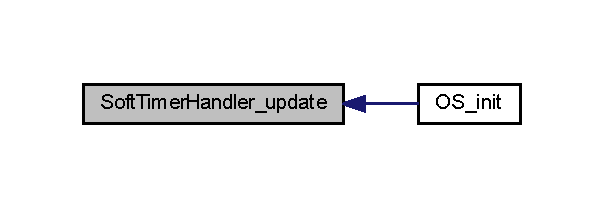
\includegraphics[width=290pt]{_soft_timer_8c_a158d51a820ff74bc56473d9f695f2531_icgraph}
\end{center}
\end{figure}



\hypertarget{_soft_timer_8h}{\section{src/os/\+Soft\+Timer.h File Reference}
\label{_soft_timer_8h}\index{src/os/\+Soft\+Timer.\+h@{src/os/\+Soft\+Timer.\+h}}
}


Soft\+Timer definiton.  


{\ttfamily \#include \char`\"{}Types.\+h\char`\"{}}\\*
Include dependency graph for Soft\+Timer.\+h\+:\nopagebreak
\begin{figure}[H]
\begin{center}
\leavevmode
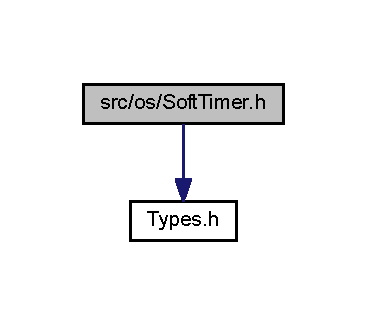
\includegraphics[width=176pt]{_soft_timer_8h__incl}
\end{center}
\end{figure}
This graph shows which files directly or indirectly include this file\+:\nopagebreak
\begin{figure}[H]
\begin{center}
\leavevmode
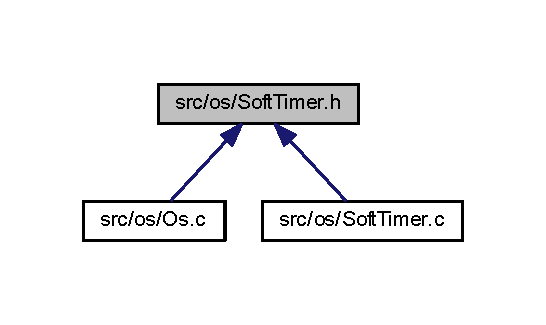
\includegraphics[width=262pt]{_soft_timer_8h__dep__incl}
\end{center}
\end{figure}
\subsection*{Data Structures}
\begin{DoxyCompactItemize}
\item 
struct \hyperlink{structtag___soft_timer}{tag\+\_\+\+Soft\+Timer}
\begin{DoxyCompactList}\small\item\em Soft\+Timer data structure. \end{DoxyCompactList}\end{DoxyCompactItemize}
\subsection*{Macros}
\begin{DoxyCompactItemize}
\item 
\hypertarget{_soft_timer_8h_a8f3ce7bf0fd80a03ad7db9c9ae3434f9}{\#define \hyperlink{_soft_timer_8h_a8f3ce7bf0fd80a03ad7db9c9ae3434f9}{S\+O\+F\+T\+T\+I\+M\+E\+R\+\_\+\+I\+S\+\_\+\+E\+X\+P\+I\+R\+E\+D}(p\+Soft\+Timer)~((0 == (p\+Soft\+Timer)-\/$>$counter) \&\& (\hyperlink{_soft_timer_8h_a745a4fd97331b42edaf70d71b104ff8faba08b201c54c6665952281a5d21bae4b}{S\+O\+F\+T\+\_\+\+T\+I\+M\+E\+R\+\_\+\+R\+U\+N\+N\+I\+N\+G} == (p\+Soft\+Timer)-\/$>$state))}\label{_soft_timer_8h_a8f3ce7bf0fd80a03ad7db9c9ae3434f9}

\begin{DoxyCompactList}\small\item\em Check if timer is expired. \end{DoxyCompactList}\end{DoxyCompactItemize}
\subsection*{Typedefs}
\begin{DoxyCompactItemize}
\item 
\hypertarget{_soft_timer_8h_a7f078e1503ae2d931bfbc6ada2145fed}{typedef enum \hyperlink{_soft_timer_8h_a745a4fd97331b42edaf70d71b104ff8f}{tag\+\_\+\+Soft\+Timer\+State} \hyperlink{_soft_timer_8h_a7f078e1503ae2d931bfbc6ada2145fed}{Soft\+Timer\+State}}\label{_soft_timer_8h_a7f078e1503ae2d931bfbc6ada2145fed}

\begin{DoxyCompactList}\small\item\em Soft\+Timer states. \end{DoxyCompactList}\item 
\hypertarget{_soft_timer_8h_a5e4ffe7f5109549a43b9971bafa8f614}{typedef struct \hyperlink{structtag___soft_timer}{tag\+\_\+\+Soft\+Timer} \hyperlink{_soft_timer_8h_a5e4ffe7f5109549a43b9971bafa8f614}{Soft\+Timer}}\label{_soft_timer_8h_a5e4ffe7f5109549a43b9971bafa8f614}

\begin{DoxyCompactList}\small\item\em Soft\+Timer data structure. \end{DoxyCompactList}\end{DoxyCompactItemize}
\subsection*{Enumerations}
\begin{DoxyCompactItemize}
\item 
enum \hyperlink{_soft_timer_8h_a58342871750337e1b043e19e4e565204}{Soft\+Timer\+\_\+\+Ret} \{ \\*
\hyperlink{_soft_timer_8h_a58342871750337e1b043e19e4e565204af209b166592ce7700937bfc2c6f4b7c8}{S\+O\+F\+T\+T\+I\+M\+E\+R\+\_\+\+R\+E\+T\+\_\+\+S\+U\+C\+C\+E\+S\+S} = 0, 
\hyperlink{_soft_timer_8h_a58342871750337e1b043e19e4e565204afe7599247a4e64c9bf9f33e5eb4cdd3a}{S\+O\+F\+T\+T\+I\+M\+E\+R\+\_\+\+R\+E\+T\+\_\+\+F\+A\+I\+L}, 
\hyperlink{_soft_timer_8h_a58342871750337e1b043e19e4e565204a1b1880e425115e61c03b6fe4936dec1e}{S\+O\+F\+T\+T\+I\+M\+E\+R\+\_\+\+R\+E\+T\+\_\+\+N\+O\+M\+O\+R\+E\+T\+I\+M\+E\+R\+S}, 
\hyperlink{_soft_timer_8h_a58342871750337e1b043e19e4e565204a224721c1ab3ae00c474fa5691406c2b7}{S\+O\+F\+T\+T\+I\+M\+E\+R\+\_\+\+R\+E\+T\+\_\+\+U\+N\+K\+N\+O\+W\+N\+T\+I\+M\+E\+R}, 
\\*
\hyperlink{_soft_timer_8h_a58342871750337e1b043e19e4e565204a2cc22debd063b9ffed80557c25c588d9}{S\+O\+F\+T\+T\+I\+M\+E\+R\+\_\+\+R\+E\+T\+\_\+\+A\+L\+R\+E\+A\+D\+Y\+R\+E\+G\+I\+S\+T\+E\+R\+E\+D}, 
\hyperlink{_soft_timer_8h_a58342871750337e1b043e19e4e565204a3e59e4ff6243dda2654e91c27b2e7a79}{S\+O\+F\+T\+T\+I\+M\+E\+R\+\_\+\+R\+E\+T\+\_\+\+N\+O\+T\+R\+E\+G\+I\+S\+T\+E\+R\+E\+D}
 \}
\begin{DoxyCompactList}\small\item\em Statuses of the soft timer api. \end{DoxyCompactList}\item 
enum \hyperlink{_soft_timer_8h_a745a4fd97331b42edaf70d71b104ff8f}{tag\+\_\+\+Soft\+Timer\+State} \{ \hyperlink{_soft_timer_8h_a745a4fd97331b42edaf70d71b104ff8fa9f44fef296f11747e45ed9e44adc3a24}{S\+O\+F\+T\+\_\+\+T\+I\+M\+E\+R\+\_\+\+U\+N\+R\+E\+G\+I\+S\+T\+E\+R\+E\+D} = 0, 
\hyperlink{_soft_timer_8h_a745a4fd97331b42edaf70d71b104ff8fab96a4e8b74b9adb07c757cc81c06fe22}{S\+O\+F\+T\+\_\+\+T\+I\+M\+E\+R\+\_\+\+S\+T\+O\+P\+P\+E\+D}, 
\hyperlink{_soft_timer_8h_a745a4fd97331b42edaf70d71b104ff8faba08b201c54c6665952281a5d21bae4b}{S\+O\+F\+T\+\_\+\+T\+I\+M\+E\+R\+\_\+\+R\+U\+N\+N\+I\+N\+G}
 \}
\begin{DoxyCompactList}\small\item\em Soft\+Timer states. \end{DoxyCompactList}\end{DoxyCompactItemize}
\subsection*{Functions}
\begin{DoxyCompactItemize}
\item 
void \hyperlink{_soft_timer_8h_a7dc718cbe43429746a7bb831c867fbdc}{Soft\+Timer\+\_\+init} (\hyperlink{_soft_timer_8h_a5e4ffe7f5109549a43b9971bafa8f614}{Soft\+Timer} $\ast$p\+Soft\+Timer)
\begin{DoxyCompactList}\small\item\em Initialize a soft timer structure. \end{DoxyCompactList}\item 
\hyperlink{_soft_timer_8h_a58342871750337e1b043e19e4e565204}{Soft\+Timer\+\_\+\+Ret} \hyperlink{_soft_timer_8h_afa63b52bac28804a7a67a0aaebf1c182}{Soft\+Timer\+\_\+start} (\hyperlink{_soft_timer_8h_a5e4ffe7f5109549a43b9971bafa8f614}{Soft\+Timer} $\ast$p\+Soft\+Timer, \hyperlink{_types_8h_aad0fc9943ec46ed9388d30c8ebe52b77}{U\+Int16} thres\+Hold)
\begin{DoxyCompactList}\small\item\em Start a soft timer with a countdown value. \end{DoxyCompactList}\item 
\hyperlink{_soft_timer_8h_a58342871750337e1b043e19e4e565204}{Soft\+Timer\+\_\+\+Ret} \hyperlink{_soft_timer_8h_a9169331d10ecae626b4884804df30b61}{Soft\+Timer\+\_\+\+Stop} (\hyperlink{_soft_timer_8h_a5e4ffe7f5109549a43b9971bafa8f614}{Soft\+Timer} $\ast$p\+Soft\+Timer)
\begin{DoxyCompactList}\small\item\em Update a soft timer (interrupt context!). \end{DoxyCompactList}\item 
void \hyperlink{_soft_timer_8h_a43d0fbf6361bd5b7d5d67bc8879f068d}{Soft\+Timer\+\_\+\+Update} (\hyperlink{_soft_timer_8h_a5e4ffe7f5109549a43b9971bafa8f614}{Soft\+Timer} $\ast$p\+Soft\+Timer)
\begin{DoxyCompactList}\small\item\em Update a soft timer (interrupt context!). \end{DoxyCompactList}\item 
\hyperlink{_soft_timer_8h_a58342871750337e1b043e19e4e565204}{Soft\+Timer\+\_\+\+Ret} \hyperlink{_soft_timer_8h_af65202ec6e69ab0744e2a942b001419c}{Soft\+Timer\+\_\+restart} (\hyperlink{_soft_timer_8h_a5e4ffe7f5109549a43b9971bafa8f614}{Soft\+Timer} $\ast$p\+Soft\+Timer)
\begin{DoxyCompactList}\small\item\em Update a soft timer with thresh\+Hold from former start call. \end{DoxyCompactList}\item 
\hyperlink{_types_8h_aad0fc9943ec46ed9388d30c8ebe52b77}{U\+Int16} \hyperlink{_soft_timer_8h_a3ebeed43ab2994f280616c02f0232a79}{Soft\+Timer\+\_\+get} (\hyperlink{_soft_timer_8h_a5e4ffe7f5109549a43b9971bafa8f614}{Soft\+Timer} $\ast$p\+Soft\+Timer)
\begin{DoxyCompactList}\small\item\em Get current countdown value of a soft timer. \end{DoxyCompactList}\item 
\hypertarget{_soft_timer_8h_a15e765af07b229a5925e5159c315fb52}{void \hyperlink{_soft_timer_8h_a15e765af07b229a5925e5159c315fb52}{Soft\+Timer\+Handler\+\_\+init} (void)}\label{_soft_timer_8h_a15e765af07b229a5925e5159c315fb52}

\begin{DoxyCompactList}\small\item\em Initialize the soft timer handler. \end{DoxyCompactList}\item 
\hyperlink{_soft_timer_8h_a58342871750337e1b043e19e4e565204}{Soft\+Timer\+\_\+\+Ret} \hyperlink{_soft_timer_8h_abe69cfc7d0e2b37de4ef7b58aae4eded}{Soft\+Timer\+Handler\+\_\+register} (\hyperlink{_soft_timer_8h_a5e4ffe7f5109549a43b9971bafa8f614}{Soft\+Timer} $\ast$p\+Soft\+Timer)
\begin{DoxyCompactList}\small\item\em Register a soft timer with the handler. \end{DoxyCompactList}\item 
\hyperlink{_soft_timer_8h_a58342871750337e1b043e19e4e565204}{Soft\+Timer\+\_\+\+Ret} \hyperlink{_soft_timer_8h_ab16250c90877e1284f842847c6aefefb}{Soft\+Timer\+Handler\+\_\+un\+Register} (\hyperlink{_soft_timer_8h_a5e4ffe7f5109549a43b9971bafa8f614}{Soft\+Timer} $\ast$p\+Soft\+Timer)
\begin{DoxyCompactList}\small\item\em De-\/\+Register a soft timer from the handler. \end{DoxyCompactList}\item 
void \hyperlink{_soft_timer_8h_a1cbbe3ecc12c3d921bc3f6b2798ba2cb}{Soft\+Timer\+Handler\+\_\+update} (void)
\begin{DoxyCompactList}\small\item\em Update all registered soft timer (interrupt context!). \end{DoxyCompactList}\item 
\hyperlink{_types_8h_aa1d7d331b6d522d6d9840fece27108d8}{U\+Int64} \hyperlink{_soft_timer_8h_a6f037f88705d2c2c5ffc621b9fd85722}{Soft\+Timer\+\_\+get\+Timestamp\+Ms} (void)
\begin{DoxyCompactList}\small\item\em Get the current value of the tick Counter in micro seconds since startup. \end{DoxyCompactList}\end{DoxyCompactItemize}


\subsection{Detailed Description}
Soft\+Timer definiton. 

A soft timer is a countdown Object that can be in state running or stopped. The countdown value is decremented in running state during every hardware timer tick until zero is reached to indicate an expired timer.

\begin{DoxyVersion}{Version}
\$\+Id\+: \hyperlink{_soft_timer_8h}{Soft\+Timer.\+h} 281 2024-\/01-\/12 12\+:09\+:03\+Z leglaz \$ 
\end{DoxyVersion}


\subsection{Enumeration Type Documentation}
\hypertarget{_soft_timer_8h_a58342871750337e1b043e19e4e565204}{\index{Soft\+Timer.\+h@{Soft\+Timer.\+h}!Soft\+Timer\+\_\+\+Ret@{Soft\+Timer\+\_\+\+Ret}}
\index{Soft\+Timer\+\_\+\+Ret@{Soft\+Timer\+\_\+\+Ret}!Soft\+Timer.\+h@{Soft\+Timer.\+h}}
\subsubsection[{Soft\+Timer\+\_\+\+Ret}]{\setlength{\rightskip}{0pt plus 5cm}enum {\bf Soft\+Timer\+\_\+\+Ret}}}\label{_soft_timer_8h_a58342871750337e1b043e19e4e565204}


Statuses of the soft timer api. 

\begin{Desc}
\item[Enumerator]\par
\begin{description}
\index{S\+O\+F\+T\+T\+I\+M\+E\+R\+\_\+\+R\+E\+T\+\_\+\+S\+U\+C\+C\+E\+S\+S@{S\+O\+F\+T\+T\+I\+M\+E\+R\+\_\+\+R\+E\+T\+\_\+\+S\+U\+C\+C\+E\+S\+S}!Soft\+Timer.\+h@{Soft\+Timer.\+h}}\index{Soft\+Timer.\+h@{Soft\+Timer.\+h}!S\+O\+F\+T\+T\+I\+M\+E\+R\+\_\+\+R\+E\+T\+\_\+\+S\+U\+C\+C\+E\+S\+S@{S\+O\+F\+T\+T\+I\+M\+E\+R\+\_\+\+R\+E\+T\+\_\+\+S\+U\+C\+C\+E\+S\+S}}\item[{\em 
\hypertarget{_soft_timer_8h_a58342871750337e1b043e19e4e565204af209b166592ce7700937bfc2c6f4b7c8}{S\+O\+F\+T\+T\+I\+M\+E\+R\+\_\+\+R\+E\+T\+\_\+\+S\+U\+C\+C\+E\+S\+S}\label{_soft_timer_8h_a58342871750337e1b043e19e4e565204af209b166592ce7700937bfc2c6f4b7c8}
}]Operation succesful. \index{S\+O\+F\+T\+T\+I\+M\+E\+R\+\_\+\+R\+E\+T\+\_\+\+F\+A\+I\+L@{S\+O\+F\+T\+T\+I\+M\+E\+R\+\_\+\+R\+E\+T\+\_\+\+F\+A\+I\+L}!Soft\+Timer.\+h@{Soft\+Timer.\+h}}\index{Soft\+Timer.\+h@{Soft\+Timer.\+h}!S\+O\+F\+T\+T\+I\+M\+E\+R\+\_\+\+R\+E\+T\+\_\+\+F\+A\+I\+L@{S\+O\+F\+T\+T\+I\+M\+E\+R\+\_\+\+R\+E\+T\+\_\+\+F\+A\+I\+L}}\item[{\em 
\hypertarget{_soft_timer_8h_a58342871750337e1b043e19e4e565204afe7599247a4e64c9bf9f33e5eb4cdd3a}{S\+O\+F\+T\+T\+I\+M\+E\+R\+\_\+\+R\+E\+T\+\_\+\+F\+A\+I\+L}\label{_soft_timer_8h_a58342871750337e1b043e19e4e565204afe7599247a4e64c9bf9f33e5eb4cdd3a}
}]Operation failed. \index{S\+O\+F\+T\+T\+I\+M\+E\+R\+\_\+\+R\+E\+T\+\_\+\+N\+O\+M\+O\+R\+E\+T\+I\+M\+E\+R\+S@{S\+O\+F\+T\+T\+I\+M\+E\+R\+\_\+\+R\+E\+T\+\_\+\+N\+O\+M\+O\+R\+E\+T\+I\+M\+E\+R\+S}!Soft\+Timer.\+h@{Soft\+Timer.\+h}}\index{Soft\+Timer.\+h@{Soft\+Timer.\+h}!S\+O\+F\+T\+T\+I\+M\+E\+R\+\_\+\+R\+E\+T\+\_\+\+N\+O\+M\+O\+R\+E\+T\+I\+M\+E\+R\+S@{S\+O\+F\+T\+T\+I\+M\+E\+R\+\_\+\+R\+E\+T\+\_\+\+N\+O\+M\+O\+R\+E\+T\+I\+M\+E\+R\+S}}\item[{\em 
\hypertarget{_soft_timer_8h_a58342871750337e1b043e19e4e565204a1b1880e425115e61c03b6fe4936dec1e}{S\+O\+F\+T\+T\+I\+M\+E\+R\+\_\+\+R\+E\+T\+\_\+\+N\+O\+M\+O\+R\+E\+T\+I\+M\+E\+R\+S}\label{_soft_timer_8h_a58342871750337e1b043e19e4e565204a1b1880e425115e61c03b6fe4936dec1e}
}]Maximum number of registered timers reached. \index{S\+O\+F\+T\+T\+I\+M\+E\+R\+\_\+\+R\+E\+T\+\_\+\+U\+N\+K\+N\+O\+W\+N\+T\+I\+M\+E\+R@{S\+O\+F\+T\+T\+I\+M\+E\+R\+\_\+\+R\+E\+T\+\_\+\+U\+N\+K\+N\+O\+W\+N\+T\+I\+M\+E\+R}!Soft\+Timer.\+h@{Soft\+Timer.\+h}}\index{Soft\+Timer.\+h@{Soft\+Timer.\+h}!S\+O\+F\+T\+T\+I\+M\+E\+R\+\_\+\+R\+E\+T\+\_\+\+U\+N\+K\+N\+O\+W\+N\+T\+I\+M\+E\+R@{S\+O\+F\+T\+T\+I\+M\+E\+R\+\_\+\+R\+E\+T\+\_\+\+U\+N\+K\+N\+O\+W\+N\+T\+I\+M\+E\+R}}\item[{\em 
\hypertarget{_soft_timer_8h_a58342871750337e1b043e19e4e565204a224721c1ab3ae00c474fa5691406c2b7}{S\+O\+F\+T\+T\+I\+M\+E\+R\+\_\+\+R\+E\+T\+\_\+\+U\+N\+K\+N\+O\+W\+N\+T\+I\+M\+E\+R}\label{_soft_timer_8h_a58342871750337e1b043e19e4e565204a224721c1ab3ae00c474fa5691406c2b7}
}]Timer is not known. \index{S\+O\+F\+T\+T\+I\+M\+E\+R\+\_\+\+R\+E\+T\+\_\+\+A\+L\+R\+E\+A\+D\+Y\+R\+E\+G\+I\+S\+T\+E\+R\+E\+D@{S\+O\+F\+T\+T\+I\+M\+E\+R\+\_\+\+R\+E\+T\+\_\+\+A\+L\+R\+E\+A\+D\+Y\+R\+E\+G\+I\+S\+T\+E\+R\+E\+D}!Soft\+Timer.\+h@{Soft\+Timer.\+h}}\index{Soft\+Timer.\+h@{Soft\+Timer.\+h}!S\+O\+F\+T\+T\+I\+M\+E\+R\+\_\+\+R\+E\+T\+\_\+\+A\+L\+R\+E\+A\+D\+Y\+R\+E\+G\+I\+S\+T\+E\+R\+E\+D@{S\+O\+F\+T\+T\+I\+M\+E\+R\+\_\+\+R\+E\+T\+\_\+\+A\+L\+R\+E\+A\+D\+Y\+R\+E\+G\+I\+S\+T\+E\+R\+E\+D}}\item[{\em 
\hypertarget{_soft_timer_8h_a58342871750337e1b043e19e4e565204a2cc22debd063b9ffed80557c25c588d9}{S\+O\+F\+T\+T\+I\+M\+E\+R\+\_\+\+R\+E\+T\+\_\+\+A\+L\+R\+E\+A\+D\+Y\+R\+E\+G\+I\+S\+T\+E\+R\+E\+D}\label{_soft_timer_8h_a58342871750337e1b043e19e4e565204a2cc22debd063b9ffed80557c25c588d9}
}]Timer is already registered. \index{S\+O\+F\+T\+T\+I\+M\+E\+R\+\_\+\+R\+E\+T\+\_\+\+N\+O\+T\+R\+E\+G\+I\+S\+T\+E\+R\+E\+D@{S\+O\+F\+T\+T\+I\+M\+E\+R\+\_\+\+R\+E\+T\+\_\+\+N\+O\+T\+R\+E\+G\+I\+S\+T\+E\+R\+E\+D}!Soft\+Timer.\+h@{Soft\+Timer.\+h}}\index{Soft\+Timer.\+h@{Soft\+Timer.\+h}!S\+O\+F\+T\+T\+I\+M\+E\+R\+\_\+\+R\+E\+T\+\_\+\+N\+O\+T\+R\+E\+G\+I\+S\+T\+E\+R\+E\+D@{S\+O\+F\+T\+T\+I\+M\+E\+R\+\_\+\+R\+E\+T\+\_\+\+N\+O\+T\+R\+E\+G\+I\+S\+T\+E\+R\+E\+D}}\item[{\em 
\hypertarget{_soft_timer_8h_a58342871750337e1b043e19e4e565204a3e59e4ff6243dda2654e91c27b2e7a79}{S\+O\+F\+T\+T\+I\+M\+E\+R\+\_\+\+R\+E\+T\+\_\+\+N\+O\+T\+R\+E\+G\+I\+S\+T\+E\+R\+E\+D}\label{_soft_timer_8h_a58342871750337e1b043e19e4e565204a3e59e4ff6243dda2654e91c27b2e7a79}
}]Timer is not registered. \end{description}
\end{Desc}
\hypertarget{_soft_timer_8h_a745a4fd97331b42edaf70d71b104ff8f}{\index{Soft\+Timer.\+h@{Soft\+Timer.\+h}!tag\+\_\+\+Soft\+Timer\+State@{tag\+\_\+\+Soft\+Timer\+State}}
\index{tag\+\_\+\+Soft\+Timer\+State@{tag\+\_\+\+Soft\+Timer\+State}!Soft\+Timer.\+h@{Soft\+Timer.\+h}}
\subsubsection[{tag\+\_\+\+Soft\+Timer\+State}]{\setlength{\rightskip}{0pt plus 5cm}enum {\bf tag\+\_\+\+Soft\+Timer\+State}}}\label{_soft_timer_8h_a745a4fd97331b42edaf70d71b104ff8f}


Soft\+Timer states. 

\begin{Desc}
\item[Enumerator]\par
\begin{description}
\index{S\+O\+F\+T\+\_\+\+T\+I\+M\+E\+R\+\_\+\+U\+N\+R\+E\+G\+I\+S\+T\+E\+R\+E\+D@{S\+O\+F\+T\+\_\+\+T\+I\+M\+E\+R\+\_\+\+U\+N\+R\+E\+G\+I\+S\+T\+E\+R\+E\+D}!Soft\+Timer.\+h@{Soft\+Timer.\+h}}\index{Soft\+Timer.\+h@{Soft\+Timer.\+h}!S\+O\+F\+T\+\_\+\+T\+I\+M\+E\+R\+\_\+\+U\+N\+R\+E\+G\+I\+S\+T\+E\+R\+E\+D@{S\+O\+F\+T\+\_\+\+T\+I\+M\+E\+R\+\_\+\+U\+N\+R\+E\+G\+I\+S\+T\+E\+R\+E\+D}}\item[{\em 
\hypertarget{_soft_timer_8h_a745a4fd97331b42edaf70d71b104ff8fa9f44fef296f11747e45ed9e44adc3a24}{S\+O\+F\+T\+\_\+\+T\+I\+M\+E\+R\+\_\+\+U\+N\+R\+E\+G\+I\+S\+T\+E\+R\+E\+D}\label{_soft_timer_8h_a745a4fd97331b42edaf70d71b104ff8fa9f44fef296f11747e45ed9e44adc3a24}
}]State unregistered. \index{S\+O\+F\+T\+\_\+\+T\+I\+M\+E\+R\+\_\+\+S\+T\+O\+P\+P\+E\+D@{S\+O\+F\+T\+\_\+\+T\+I\+M\+E\+R\+\_\+\+S\+T\+O\+P\+P\+E\+D}!Soft\+Timer.\+h@{Soft\+Timer.\+h}}\index{Soft\+Timer.\+h@{Soft\+Timer.\+h}!S\+O\+F\+T\+\_\+\+T\+I\+M\+E\+R\+\_\+\+S\+T\+O\+P\+P\+E\+D@{S\+O\+F\+T\+\_\+\+T\+I\+M\+E\+R\+\_\+\+S\+T\+O\+P\+P\+E\+D}}\item[{\em 
\hypertarget{_soft_timer_8h_a745a4fd97331b42edaf70d71b104ff8fab96a4e8b74b9adb07c757cc81c06fe22}{S\+O\+F\+T\+\_\+\+T\+I\+M\+E\+R\+\_\+\+S\+T\+O\+P\+P\+E\+D}\label{_soft_timer_8h_a745a4fd97331b42edaf70d71b104ff8fab96a4e8b74b9adb07c757cc81c06fe22}
}]State stopped. \index{S\+O\+F\+T\+\_\+\+T\+I\+M\+E\+R\+\_\+\+R\+U\+N\+N\+I\+N\+G@{S\+O\+F\+T\+\_\+\+T\+I\+M\+E\+R\+\_\+\+R\+U\+N\+N\+I\+N\+G}!Soft\+Timer.\+h@{Soft\+Timer.\+h}}\index{Soft\+Timer.\+h@{Soft\+Timer.\+h}!S\+O\+F\+T\+\_\+\+T\+I\+M\+E\+R\+\_\+\+R\+U\+N\+N\+I\+N\+G@{S\+O\+F\+T\+\_\+\+T\+I\+M\+E\+R\+\_\+\+R\+U\+N\+N\+I\+N\+G}}\item[{\em 
\hypertarget{_soft_timer_8h_a745a4fd97331b42edaf70d71b104ff8faba08b201c54c6665952281a5d21bae4b}{S\+O\+F\+T\+\_\+\+T\+I\+M\+E\+R\+\_\+\+R\+U\+N\+N\+I\+N\+G}\label{_soft_timer_8h_a745a4fd97331b42edaf70d71b104ff8faba08b201c54c6665952281a5d21bae4b}
}]State running. \end{description}
\end{Desc}


\subsection{Function Documentation}
\hypertarget{_soft_timer_8h_a3ebeed43ab2994f280616c02f0232a79}{\index{Soft\+Timer.\+h@{Soft\+Timer.\+h}!Soft\+Timer\+\_\+get@{Soft\+Timer\+\_\+get}}
\index{Soft\+Timer\+\_\+get@{Soft\+Timer\+\_\+get}!Soft\+Timer.\+h@{Soft\+Timer.\+h}}
\subsubsection[{Soft\+Timer\+\_\+get}]{\setlength{\rightskip}{0pt plus 5cm}{\bf U\+Int16} Soft\+Timer\+\_\+get (
\begin{DoxyParamCaption}
\item[{{\bf Soft\+Timer} $\ast$}]{p\+Soft\+Timer}
\end{DoxyParamCaption}
)}}\label{_soft_timer_8h_a3ebeed43ab2994f280616c02f0232a79}


Get current countdown value of a soft timer. 


\begin{DoxyParams}[1]{Parameters}
\mbox{\tt in}  & {\em p\+Soft\+Timer} & A soft timer structure. \\
\hline
\end{DoxyParams}


References tag\+\_\+\+Soft\+Timer\+::counter.

\hypertarget{_soft_timer_8h_a6f037f88705d2c2c5ffc621b9fd85722}{\index{Soft\+Timer.\+h@{Soft\+Timer.\+h}!Soft\+Timer\+\_\+get\+Timestamp\+Ms@{Soft\+Timer\+\_\+get\+Timestamp\+Ms}}
\index{Soft\+Timer\+\_\+get\+Timestamp\+Ms@{Soft\+Timer\+\_\+get\+Timestamp\+Ms}!Soft\+Timer.\+h@{Soft\+Timer.\+h}}
\subsubsection[{Soft\+Timer\+\_\+get\+Timestamp\+Ms}]{\setlength{\rightskip}{0pt plus 5cm}{\bf U\+Int64} Soft\+Timer\+\_\+get\+Timestamp\+Ms (
\begin{DoxyParamCaption}
\item[{void}]{}
\end{DoxyParamCaption}
)}}\label{_soft_timer_8h_a6f037f88705d2c2c5ffc621b9fd85722}


Get the current value of the tick Counter in micro seconds since startup. 

\begin{DoxyReturn}{Returns}
tick counter value in microseconds. 
\end{DoxyReturn}
\hypertarget{_soft_timer_8h_a7dc718cbe43429746a7bb831c867fbdc}{\index{Soft\+Timer.\+h@{Soft\+Timer.\+h}!Soft\+Timer\+\_\+init@{Soft\+Timer\+\_\+init}}
\index{Soft\+Timer\+\_\+init@{Soft\+Timer\+\_\+init}!Soft\+Timer.\+h@{Soft\+Timer.\+h}}
\subsubsection[{Soft\+Timer\+\_\+init}]{\setlength{\rightskip}{0pt plus 5cm}void Soft\+Timer\+\_\+init (
\begin{DoxyParamCaption}
\item[{{\bf Soft\+Timer} $\ast$}]{p\+Soft\+Timer}
\end{DoxyParamCaption}
)}}\label{_soft_timer_8h_a7dc718cbe43429746a7bb831c867fbdc}


Initialize a soft timer structure. 


\begin{DoxyParams}[1]{Parameters}
\mbox{\tt in}  & {\em p\+Soft\+Timer} & A soft timer structure. \\
\hline
\end{DoxyParams}


References tag\+\_\+\+Soft\+Timer\+::counter, S\+O\+F\+T\+\_\+\+T\+I\+M\+E\+R\+\_\+\+U\+N\+R\+E\+G\+I\+S\+T\+E\+R\+E\+D, tag\+\_\+\+Soft\+Timer\+::state, and tag\+\_\+\+Soft\+Timer\+::thresh\+Hold.

\hypertarget{_soft_timer_8h_af65202ec6e69ab0744e2a942b001419c}{\index{Soft\+Timer.\+h@{Soft\+Timer.\+h}!Soft\+Timer\+\_\+restart@{Soft\+Timer\+\_\+restart}}
\index{Soft\+Timer\+\_\+restart@{Soft\+Timer\+\_\+restart}!Soft\+Timer.\+h@{Soft\+Timer.\+h}}
\subsubsection[{Soft\+Timer\+\_\+restart}]{\setlength{\rightskip}{0pt plus 5cm}{\bf Soft\+Timer\+\_\+\+Ret} Soft\+Timer\+\_\+restart (
\begin{DoxyParamCaption}
\item[{{\bf Soft\+Timer} $\ast$}]{p\+Soft\+Timer}
\end{DoxyParamCaption}
)}}\label{_soft_timer_8h_af65202ec6e69ab0744e2a942b001419c}


Update a soft timer with thresh\+Hold from former start call. 


\begin{DoxyParams}[1]{Parameters}
\mbox{\tt in}  & {\em p\+Soft\+Timer} & A soft timer structure. \\
\hline
\end{DoxyParams}


References Soft\+Timer\+\_\+start(), and tag\+\_\+\+Soft\+Timer\+::thresh\+Hold.



Here is the call graph for this function\+:\nopagebreak
\begin{figure}[H]
\begin{center}
\leavevmode
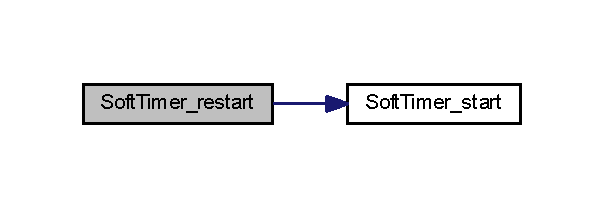
\includegraphics[width=290pt]{_soft_timer_8h_af65202ec6e69ab0744e2a942b001419c_cgraph}
\end{center}
\end{figure}


\hypertarget{_soft_timer_8h_afa63b52bac28804a7a67a0aaebf1c182}{\index{Soft\+Timer.\+h@{Soft\+Timer.\+h}!Soft\+Timer\+\_\+start@{Soft\+Timer\+\_\+start}}
\index{Soft\+Timer\+\_\+start@{Soft\+Timer\+\_\+start}!Soft\+Timer.\+h@{Soft\+Timer.\+h}}
\subsubsection[{Soft\+Timer\+\_\+start}]{\setlength{\rightskip}{0pt plus 5cm}{\bf Soft\+Timer\+\_\+\+Ret} Soft\+Timer\+\_\+start (
\begin{DoxyParamCaption}
\item[{{\bf Soft\+Timer} $\ast$}]{p\+Soft\+Timer, }
\item[{{\bf U\+Int16}}]{thres\+Hold}
\end{DoxyParamCaption}
)}}\label{_soft_timer_8h_afa63b52bac28804a7a67a0aaebf1c182}


Start a soft timer with a countdown value. 


\begin{DoxyParams}[1]{Parameters}
\mbox{\tt in}  & {\em p\+Soft\+Timer} & A soft timer structure. \\
\hline
\mbox{\tt in}  & {\em thres\+Hold} & The start value of the count down. \\
\hline
\end{DoxyParams}


References tag\+\_\+\+Soft\+Timer\+::counter, S\+O\+F\+T\+\_\+\+T\+I\+M\+E\+R\+\_\+\+R\+U\+N\+N\+I\+N\+G, S\+O\+F\+T\+\_\+\+T\+I\+M\+E\+R\+\_\+\+U\+N\+R\+E\+G\+I\+S\+T\+E\+R\+E\+D, S\+O\+F\+T\+T\+I\+M\+E\+R\+\_\+\+R\+E\+T\+\_\+\+N\+O\+T\+R\+E\+G\+I\+S\+T\+E\+R\+E\+D, S\+O\+F\+T\+T\+I\+M\+E\+R\+\_\+\+R\+E\+T\+\_\+\+S\+U\+C\+C\+E\+S\+S, tag\+\_\+\+Soft\+Timer\+::state, and tag\+\_\+\+Soft\+Timer\+::thresh\+Hold.



Referenced by Soft\+Timer\+\_\+restart().



Here is the caller graph for this function\+:\nopagebreak
\begin{figure}[H]
\begin{center}
\leavevmode
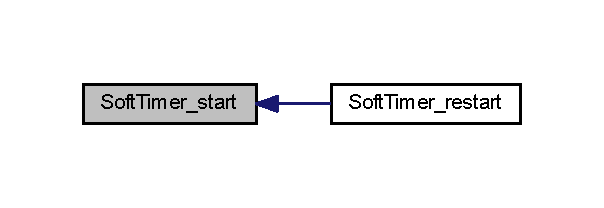
\includegraphics[width=290pt]{_soft_timer_8h_afa63b52bac28804a7a67a0aaebf1c182_icgraph}
\end{center}
\end{figure}


\hypertarget{_soft_timer_8h_a9169331d10ecae626b4884804df30b61}{\index{Soft\+Timer.\+h@{Soft\+Timer.\+h}!Soft\+Timer\+\_\+\+Stop@{Soft\+Timer\+\_\+\+Stop}}
\index{Soft\+Timer\+\_\+\+Stop@{Soft\+Timer\+\_\+\+Stop}!Soft\+Timer.\+h@{Soft\+Timer.\+h}}
\subsubsection[{Soft\+Timer\+\_\+\+Stop}]{\setlength{\rightskip}{0pt plus 5cm}{\bf Soft\+Timer\+\_\+\+Ret} Soft\+Timer\+\_\+\+Stop (
\begin{DoxyParamCaption}
\item[{{\bf Soft\+Timer} $\ast$}]{p\+Soft\+Timer}
\end{DoxyParamCaption}
)}}\label{_soft_timer_8h_a9169331d10ecae626b4884804df30b61}


Update a soft timer (interrupt context!). 


\begin{DoxyParams}[1]{Parameters}
\mbox{\tt in}  & {\em p\+Soft\+Timer} & A soft timer structure. \\
\hline
\end{DoxyParams}


References S\+O\+F\+T\+\_\+\+T\+I\+M\+E\+R\+\_\+\+S\+T\+O\+P\+P\+E\+D, S\+O\+F\+T\+\_\+\+T\+I\+M\+E\+R\+\_\+\+U\+N\+R\+E\+G\+I\+S\+T\+E\+R\+E\+D, S\+O\+F\+T\+T\+I\+M\+E\+R\+\_\+\+R\+E\+T\+\_\+\+N\+O\+T\+R\+E\+G\+I\+S\+T\+E\+R\+E\+D, S\+O\+F\+T\+T\+I\+M\+E\+R\+\_\+\+R\+E\+T\+\_\+\+S\+U\+C\+C\+E\+S\+S, and tag\+\_\+\+Soft\+Timer\+::state.

\hypertarget{_soft_timer_8h_a43d0fbf6361bd5b7d5d67bc8879f068d}{\index{Soft\+Timer.\+h@{Soft\+Timer.\+h}!Soft\+Timer\+\_\+\+Update@{Soft\+Timer\+\_\+\+Update}}
\index{Soft\+Timer\+\_\+\+Update@{Soft\+Timer\+\_\+\+Update}!Soft\+Timer.\+h@{Soft\+Timer.\+h}}
\subsubsection[{Soft\+Timer\+\_\+\+Update}]{\setlength{\rightskip}{0pt plus 5cm}void Soft\+Timer\+\_\+\+Update (
\begin{DoxyParamCaption}
\item[{{\bf Soft\+Timer} $\ast$}]{p\+Soft\+Timer}
\end{DoxyParamCaption}
)}}\label{_soft_timer_8h_a43d0fbf6361bd5b7d5d67bc8879f068d}


Update a soft timer (interrupt context!). 


\begin{DoxyParams}[1]{Parameters}
\mbox{\tt in}  & {\em p\+Soft\+Timer} & A soft timer structure. \\
\hline
\end{DoxyParams}


References tag\+\_\+\+Soft\+Timer\+::counter, S\+O\+F\+T\+\_\+\+T\+I\+M\+E\+R\+\_\+\+R\+U\+N\+N\+I\+N\+G, and tag\+\_\+\+Soft\+Timer\+::state.

\hypertarget{_soft_timer_8h_abe69cfc7d0e2b37de4ef7b58aae4eded}{\index{Soft\+Timer.\+h@{Soft\+Timer.\+h}!Soft\+Timer\+Handler\+\_\+register@{Soft\+Timer\+Handler\+\_\+register}}
\index{Soft\+Timer\+Handler\+\_\+register@{Soft\+Timer\+Handler\+\_\+register}!Soft\+Timer.\+h@{Soft\+Timer.\+h}}
\subsubsection[{Soft\+Timer\+Handler\+\_\+register}]{\setlength{\rightskip}{0pt plus 5cm}{\bf Soft\+Timer\+\_\+\+Ret} Soft\+Timer\+Handler\+\_\+register (
\begin{DoxyParamCaption}
\item[{{\bf Soft\+Timer} $\ast$}]{p\+Soft\+Timer}
\end{DoxyParamCaption}
)}}\label{_soft_timer_8h_abe69cfc7d0e2b37de4ef7b58aae4eded}


Register a soft timer with the handler. 


\begin{DoxyParams}[1]{Parameters}
\mbox{\tt in}  & {\em p\+Soft\+Timer} & A soft timer structure. \\
\hline
\end{DoxyParams}


References N\+U\+L\+L, S\+O\+F\+T\+\_\+\+T\+I\+M\+E\+R\+\_\+\+M\+A\+X\+\_\+\+T\+I\+M\+E\+R, S\+O\+F\+T\+\_\+\+T\+I\+M\+E\+R\+\_\+\+S\+T\+O\+P\+P\+E\+D, S\+O\+F\+T\+T\+I\+M\+E\+R\+\_\+\+R\+E\+T\+\_\+\+A\+L\+R\+E\+A\+D\+Y\+R\+E\+G\+I\+S\+T\+E\+R\+E\+D, S\+O\+F\+T\+T\+I\+M\+E\+R\+\_\+\+R\+E\+T\+\_\+\+N\+O\+M\+O\+R\+E\+T\+I\+M\+E\+R\+S, S\+O\+F\+T\+T\+I\+M\+E\+R\+\_\+\+R\+E\+T\+\_\+\+S\+U\+C\+C\+E\+S\+S, and tag\+\_\+\+Soft\+Timer\+::state.

\hypertarget{_soft_timer_8h_ab16250c90877e1284f842847c6aefefb}{\index{Soft\+Timer.\+h@{Soft\+Timer.\+h}!Soft\+Timer\+Handler\+\_\+un\+Register@{Soft\+Timer\+Handler\+\_\+un\+Register}}
\index{Soft\+Timer\+Handler\+\_\+un\+Register@{Soft\+Timer\+Handler\+\_\+un\+Register}!Soft\+Timer.\+h@{Soft\+Timer.\+h}}
\subsubsection[{Soft\+Timer\+Handler\+\_\+un\+Register}]{\setlength{\rightskip}{0pt plus 5cm}{\bf Soft\+Timer\+\_\+\+Ret} Soft\+Timer\+Handler\+\_\+un\+Register (
\begin{DoxyParamCaption}
\item[{{\bf Soft\+Timer} $\ast$}]{p\+Soft\+Timer}
\end{DoxyParamCaption}
)}}\label{_soft_timer_8h_ab16250c90877e1284f842847c6aefefb}


De-\/\+Register a soft timer from the handler. 


\begin{DoxyParams}[1]{Parameters}
\mbox{\tt in}  & {\em p\+Soft\+Timer} & A soft timer structure. \\
\hline
\end{DoxyParams}


References N\+U\+L\+L, S\+O\+F\+T\+\_\+\+T\+I\+M\+E\+R\+\_\+\+M\+A\+X\+\_\+\+T\+I\+M\+E\+R, S\+O\+F\+T\+T\+I\+M\+E\+R\+\_\+\+R\+E\+T\+\_\+\+S\+U\+C\+C\+E\+S\+S, and S\+O\+F\+T\+T\+I\+M\+E\+R\+\_\+\+R\+E\+T\+\_\+\+U\+N\+K\+N\+O\+W\+N\+T\+I\+M\+E\+R.

\hypertarget{_soft_timer_8h_a1cbbe3ecc12c3d921bc3f6b2798ba2cb}{\index{Soft\+Timer.\+h@{Soft\+Timer.\+h}!Soft\+Timer\+Handler\+\_\+update@{Soft\+Timer\+Handler\+\_\+update}}
\index{Soft\+Timer\+Handler\+\_\+update@{Soft\+Timer\+Handler\+\_\+update}!Soft\+Timer.\+h@{Soft\+Timer.\+h}}
\subsubsection[{Soft\+Timer\+Handler\+\_\+update}]{\setlength{\rightskip}{0pt plus 5cm}void Soft\+Timer\+Handler\+\_\+update (
\begin{DoxyParamCaption}
\item[{void}]{}
\end{DoxyParamCaption}
)}}\label{_soft_timer_8h_a1cbbe3ecc12c3d921bc3f6b2798ba2cb}


Update all registered soft timer (interrupt context!). 



References tag\+\_\+\+Soft\+Timer\+::counter, N\+U\+L\+L, S\+O\+F\+T\+\_\+\+T\+I\+M\+E\+R\+\_\+\+M\+A\+X\+\_\+\+T\+I\+M\+E\+R, S\+O\+F\+T\+\_\+\+T\+I\+M\+E\+R\+\_\+\+R\+U\+N\+N\+I\+N\+G, and tag\+\_\+\+Soft\+Timer\+::state.



Referenced by O\+S\+\_\+init().



Here is the caller graph for this function\+:\nopagebreak
\begin{figure}[H]
\begin{center}
\leavevmode
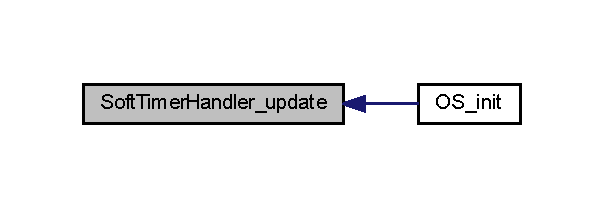
\includegraphics[width=290pt]{_soft_timer_8h_a1cbbe3ecc12c3d921bc3f6b2798ba2cb_icgraph}
\end{center}
\end{figure}



\hypertarget{_task_8c}{\section{src/os/\+Task.c File Reference}
\label{_task_8c}\index{src/os/\+Task.\+c@{src/os/\+Task.\+c}}
}


Simple task scheduler.  


{\ttfamily \#include $<$string.\+h$>$}\\*
{\ttfamily \#include \char`\"{}os/\+Task.\+h\char`\"{}}\\*
Include dependency graph for Task.\+c\+:\nopagebreak
\begin{figure}[H]
\begin{center}
\leavevmode
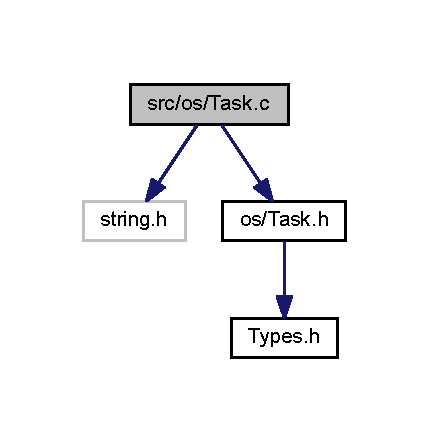
\includegraphics[width=206pt]{_task_8c__incl}
\end{center}
\end{figure}
\subsection*{Functions}
\begin{DoxyCompactItemize}
\item 
\hyperlink{_task_8h_a37f1bd0af944415ae4fa0cf9574d3ad5}{Task\+\_\+\+Ret} \hyperlink{_task_8c_a7826f67d79e978d4771d581421ba4210}{Task\+\_\+init} (\hyperlink{_task_8h_a77bbd51a2c7d34bd2aa764baadfb4b83}{Task} $\ast$p\+Task, \hyperlink{_task_8h_a8f3c61c0430299673ab83bf936073184}{Task\+Work\+Callback} callback, \hyperlink{_task_8h_a72a5e74cf680503ec09223c3cfdbf4e3}{Task\+State} state, void $\ast$data)
\begin{DoxyCompactList}\small\item\em Initialize a task structure. \end{DoxyCompactList}\end{DoxyCompactItemize}


\subsection{Detailed Description}
Simple task scheduler. 

For a detailed description see the detailed description in \hyperlink{_scheduler_8h}{Scheduler.\+h}.

\begin{DoxyVersion}{Version}
\$\+Id\+: \hyperlink{_task_8c}{Task.\+c} 281 2024-\/01-\/12 12\+:09\+:03\+Z leglaz \$ 
\end{DoxyVersion}


\subsection{Function Documentation}
\hypertarget{_task_8c_a7826f67d79e978d4771d581421ba4210}{\index{Task.\+c@{Task.\+c}!Task\+\_\+init@{Task\+\_\+init}}
\index{Task\+\_\+init@{Task\+\_\+init}!Task.\+c@{Task.\+c}}
\subsubsection[{Task\+\_\+init}]{\setlength{\rightskip}{0pt plus 5cm}{\bf Task\+\_\+\+Ret} Task\+\_\+init (
\begin{DoxyParamCaption}
\item[{{\bf Task} $\ast$}]{task, }
\item[{{\bf Task\+Work\+Callback}}]{callback, }
\item[{{\bf Task\+State}}]{state, }
\item[{void $\ast$}]{data}
\end{DoxyParamCaption}
)}}\label{_task_8c_a7826f67d79e978d4771d581421ba4210}


Initialize a task structure. 


\begin{DoxyParams}[1]{Parameters}
\mbox{\tt in}  & {\em task} & The task structure to initialize. \\
\hline
\mbox{\tt in}  & {\em callback} & The task work cycle function. \\
\hline
\mbox{\tt in}  & {\em state} & The task state. \\
\hline
\mbox{\tt in}  & {\em data} & Task context data that gets passed to the work cycle function.\\
\hline
\end{DoxyParams}
\begin{DoxyReturn}{Returns}
Task\+\_\+\+Ret Status of operation. 
\end{DoxyReturn}


References tag\+\_\+\+Task\+::instance\+Data, N\+U\+L\+L, tag\+\_\+\+Task\+::state, T\+A\+S\+K\+\_\+\+R\+E\+T\+\_\+\+F\+A\+I\+L, T\+A\+S\+K\+\_\+\+R\+E\+T\+\_\+\+S\+U\+C\+C\+E\+S\+S, and tag\+\_\+\+Task\+::work\+Callback.



Referenced by Main\+Task\+\_\+init().



Here is the caller graph for this function\+:\nopagebreak
\begin{figure}[H]
\begin{center}
\leavevmode
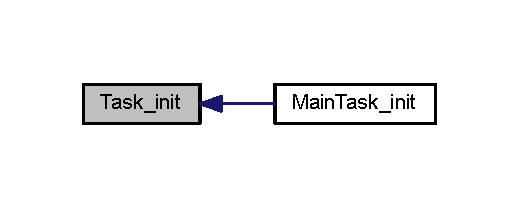
\includegraphics[width=249pt]{_task_8c_a7826f67d79e978d4771d581421ba4210_icgraph}
\end{center}
\end{figure}



\hypertarget{_task_8h}{\section{src/os/\+Task.h File Reference}
\label{_task_8h}\index{src/os/\+Task.\+h@{src/os/\+Task.\+h}}
}


Enter short description here.  


{\ttfamily \#include \char`\"{}Types.\+h\char`\"{}}\\*
Include dependency graph for Task.\+h\+:\nopagebreak
\begin{figure}[H]
\begin{center}
\leavevmode
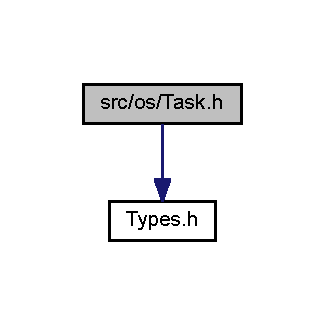
\includegraphics[width=156pt]{_task_8h__incl}
\end{center}
\end{figure}
This graph shows which files directly or indirectly include this file\+:\nopagebreak
\begin{figure}[H]
\begin{center}
\leavevmode
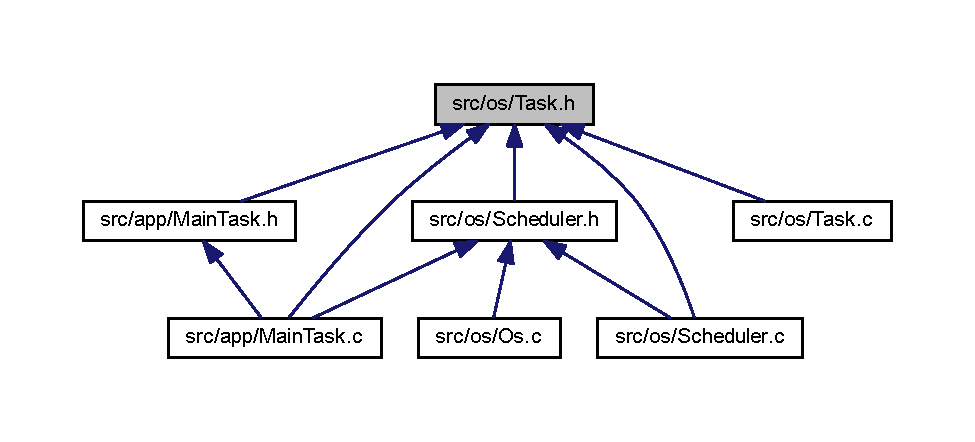
\includegraphics[width=350pt]{_task_8h__dep__incl}
\end{center}
\end{figure}
\subsection*{Data Structures}
\begin{DoxyCompactItemize}
\item 
struct \hyperlink{structtag___task}{tag\+\_\+\+Task}
\begin{DoxyCompactList}\small\item\em Task Structure. \end{DoxyCompactList}\end{DoxyCompactItemize}
\subsection*{Macros}
\begin{DoxyCompactItemize}
\item 
\#define \hyperlink{_task_8h_a1b1454a97d564dca99542ba060801e30}{T\+A\+S\+K\+\_\+\+G\+E\+T\+\_\+\+S\+T\+A\+T\+E}(task)~(task)-\/$>$state
\begin{DoxyCompactList}\small\item\em Get state of a given task. \end{DoxyCompactList}\item 
\#define \hyperlink{_task_8h_a4b05cd5351328ecb3a9ec9cbebd2ac77}{T\+A\+S\+K\+\_\+\+S\+E\+T\+\_\+\+S\+T\+A\+T\+E}(task, new\+State)~(task)-\/$>$state = (new\+State)
\begin{DoxyCompactList}\small\item\em Set state of given task. \end{DoxyCompactList}\item 
\#define \hyperlink{_task_8h_abab652c9af371c87e7a775e161ea80c5}{T\+A\+S\+K\+\_\+\+E\+X\+E\+C\+U\+T\+E}(task)~(task)-\/$>$work\+Callback((task-\/$>$instance\+Data))
\begin{DoxyCompactList}\small\item\em Execute the task work cycle function. \end{DoxyCompactList}\end{DoxyCompactItemize}
\subsection*{Typedefs}
\begin{DoxyCompactItemize}
\item 
\hypertarget{_task_8h_a72a5e74cf680503ec09223c3cfdbf4e3}{typedef enum \hyperlink{_task_8h_a729b795ce2389deacd8fbee97626723f}{tag\+\_\+\+Task\+State} \hyperlink{_task_8h_a72a5e74cf680503ec09223c3cfdbf4e3}{Task\+State}}\label{_task_8h_a72a5e74cf680503ec09223c3cfdbf4e3}

\begin{DoxyCompactList}\small\item\em Possible Task States. \end{DoxyCompactList}\item 
\hypertarget{_task_8h_a8f3c61c0430299673ab83bf936073184}{typedef void($\ast$ \hyperlink{_task_8h_a8f3c61c0430299673ab83bf936073184}{Task\+Work\+Callback} )(void $\ast$instance\+Data)}\label{_task_8h_a8f3c61c0430299673ab83bf936073184}

\begin{DoxyCompactList}\small\item\em Type of task work cycle function. \end{DoxyCompactList}\item 
\hypertarget{_task_8h_a77bbd51a2c7d34bd2aa764baadfb4b83}{typedef struct \hyperlink{structtag___task}{tag\+\_\+\+Task} \hyperlink{_task_8h_a77bbd51a2c7d34bd2aa764baadfb4b83}{Task}}\label{_task_8h_a77bbd51a2c7d34bd2aa764baadfb4b83}

\begin{DoxyCompactList}\small\item\em Task Structure. \end{DoxyCompactList}\end{DoxyCompactItemize}
\subsection*{Enumerations}
\begin{DoxyCompactItemize}
\item 
enum \hyperlink{_task_8h_a37f1bd0af944415ae4fa0cf9574d3ad5}{Task\+\_\+\+Ret} \{ \hyperlink{_task_8h_a37f1bd0af944415ae4fa0cf9574d3ad5ac6eaa84301a1ab2a52c6101b44c8a5d8}{T\+A\+S\+K\+\_\+\+R\+E\+T\+\_\+\+F\+A\+I\+L} = 0, 
\hyperlink{_task_8h_a37f1bd0af944415ae4fa0cf9574d3ad5a455a96c47d66f1cc26b316d2d05ace28}{T\+A\+S\+K\+\_\+\+R\+E\+T\+\_\+\+S\+U\+C\+C\+E\+S\+S}
 \}
\begin{DoxyCompactList}\small\item\em Statuses of the task. \end{DoxyCompactList}\item 
enum \hyperlink{_task_8h_a729b795ce2389deacd8fbee97626723f}{tag\+\_\+\+Task\+State} \{ \hyperlink{_task_8h_a729b795ce2389deacd8fbee97626723fac47ca944190c8714014acf6e55800747}{T\+A\+S\+K\+\_\+\+S\+T\+A\+T\+E\+\_\+\+S\+U\+S\+P\+E\+N\+D\+E\+D} = 0, 
\hyperlink{_task_8h_a729b795ce2389deacd8fbee97626723fa169adc0116f5c61af55d2dd88709ea4e}{T\+A\+S\+K\+\_\+\+S\+T\+A\+T\+E\+\_\+\+R\+U\+N\+N\+I\+N\+G}
 \}
\begin{DoxyCompactList}\small\item\em Possible Task States. \end{DoxyCompactList}\end{DoxyCompactItemize}
\subsection*{Functions}
\begin{DoxyCompactItemize}
\item 
\hyperlink{_task_8h_a37f1bd0af944415ae4fa0cf9574d3ad5}{Task\+\_\+\+Ret} \hyperlink{_task_8h_a4b074cf85d0db22ecd5abd511c33a2c4}{Task\+\_\+init} (\hyperlink{_task_8h_a77bbd51a2c7d34bd2aa764baadfb4b83}{Task} $\ast$task, \hyperlink{_task_8h_a8f3c61c0430299673ab83bf936073184}{Task\+Work\+Callback} callback, \hyperlink{_task_8h_a72a5e74cf680503ec09223c3cfdbf4e3}{Task\+State} state, void $\ast$data)
\begin{DoxyCompactList}\small\item\em Initialize a task structure. \end{DoxyCompactList}\end{DoxyCompactItemize}


\subsection{Detailed Description}
Enter short description here. 

Enter detailed description here.

\begin{DoxyVersion}{Version}
\$\+Id\+: \hyperlink{_task_8h}{Task.\+h} 281 2024-\/01-\/12 12\+:09\+:03\+Z leglaz \$ 
\end{DoxyVersion}


\subsection{Macro Definition Documentation}
\hypertarget{_task_8h_abab652c9af371c87e7a775e161ea80c5}{\index{Task.\+h@{Task.\+h}!T\+A\+S\+K\+\_\+\+E\+X\+E\+C\+U\+T\+E@{T\+A\+S\+K\+\_\+\+E\+X\+E\+C\+U\+T\+E}}
\index{T\+A\+S\+K\+\_\+\+E\+X\+E\+C\+U\+T\+E@{T\+A\+S\+K\+\_\+\+E\+X\+E\+C\+U\+T\+E}!Task.\+h@{Task.\+h}}
\subsubsection[{T\+A\+S\+K\+\_\+\+E\+X\+E\+C\+U\+T\+E}]{\setlength{\rightskip}{0pt plus 5cm}\#define T\+A\+S\+K\+\_\+\+E\+X\+E\+C\+U\+T\+E(
\begin{DoxyParamCaption}
\item[{}]{task}
\end{DoxyParamCaption}
)~(task)-\/$>$work\+Callback((task-\/$>$instance\+Data))}}\label{_task_8h_abab652c9af371c87e7a775e161ea80c5}


Execute the task work cycle function. 


\begin{DoxyParams}[1]{Parameters}
\mbox{\tt in}  & {\em task} & Pointer to task structure. \\
\hline
\end{DoxyParams}


Referenced by Scheduler\+\_\+execute().

\hypertarget{_task_8h_a1b1454a97d564dca99542ba060801e30}{\index{Task.\+h@{Task.\+h}!T\+A\+S\+K\+\_\+\+G\+E\+T\+\_\+\+S\+T\+A\+T\+E@{T\+A\+S\+K\+\_\+\+G\+E\+T\+\_\+\+S\+T\+A\+T\+E}}
\index{T\+A\+S\+K\+\_\+\+G\+E\+T\+\_\+\+S\+T\+A\+T\+E@{T\+A\+S\+K\+\_\+\+G\+E\+T\+\_\+\+S\+T\+A\+T\+E}!Task.\+h@{Task.\+h}}
\subsubsection[{T\+A\+S\+K\+\_\+\+G\+E\+T\+\_\+\+S\+T\+A\+T\+E}]{\setlength{\rightskip}{0pt plus 5cm}\#define T\+A\+S\+K\+\_\+\+G\+E\+T\+\_\+\+S\+T\+A\+T\+E(
\begin{DoxyParamCaption}
\item[{}]{task}
\end{DoxyParamCaption}
)~(task)-\/$>$state}}\label{_task_8h_a1b1454a97d564dca99542ba060801e30}


Get state of a given task. 


\begin{DoxyParams}[1]{Parameters}
\mbox{\tt in}  & {\em task} & Pointer to task structure. \\
\hline
\end{DoxyParams}


Referenced by Scheduler\+\_\+execute().

\hypertarget{_task_8h_a4b05cd5351328ecb3a9ec9cbebd2ac77}{\index{Task.\+h@{Task.\+h}!T\+A\+S\+K\+\_\+\+S\+E\+T\+\_\+\+S\+T\+A\+T\+E@{T\+A\+S\+K\+\_\+\+S\+E\+T\+\_\+\+S\+T\+A\+T\+E}}
\index{T\+A\+S\+K\+\_\+\+S\+E\+T\+\_\+\+S\+T\+A\+T\+E@{T\+A\+S\+K\+\_\+\+S\+E\+T\+\_\+\+S\+T\+A\+T\+E}!Task.\+h@{Task.\+h}}
\subsubsection[{T\+A\+S\+K\+\_\+\+S\+E\+T\+\_\+\+S\+T\+A\+T\+E}]{\setlength{\rightskip}{0pt plus 5cm}\#define T\+A\+S\+K\+\_\+\+S\+E\+T\+\_\+\+S\+T\+A\+T\+E(
\begin{DoxyParamCaption}
\item[{}]{task, }
\item[{}]{new\+State}
\end{DoxyParamCaption}
)~(task)-\/$>$state = (new\+State)}}\label{_task_8h_a4b05cd5351328ecb3a9ec9cbebd2ac77}


Set state of given task. 


\begin{DoxyParams}[1]{Parameters}
\mbox{\tt in}  & {\em task} & Pointer to task structure. \\
\hline
\mbox{\tt in}  & {\em new\+State} & New task state. \\
\hline
\end{DoxyParams}


\subsection{Enumeration Type Documentation}
\hypertarget{_task_8h_a729b795ce2389deacd8fbee97626723f}{\index{Task.\+h@{Task.\+h}!tag\+\_\+\+Task\+State@{tag\+\_\+\+Task\+State}}
\index{tag\+\_\+\+Task\+State@{tag\+\_\+\+Task\+State}!Task.\+h@{Task.\+h}}
\subsubsection[{tag\+\_\+\+Task\+State}]{\setlength{\rightskip}{0pt plus 5cm}enum {\bf tag\+\_\+\+Task\+State}}}\label{_task_8h_a729b795ce2389deacd8fbee97626723f}


Possible Task States. 

\begin{Desc}
\item[Enumerator]\par
\begin{description}
\index{T\+A\+S\+K\+\_\+\+S\+T\+A\+T\+E\+\_\+\+S\+U\+S\+P\+E\+N\+D\+E\+D@{T\+A\+S\+K\+\_\+\+S\+T\+A\+T\+E\+\_\+\+S\+U\+S\+P\+E\+N\+D\+E\+D}!Task.\+h@{Task.\+h}}\index{Task.\+h@{Task.\+h}!T\+A\+S\+K\+\_\+\+S\+T\+A\+T\+E\+\_\+\+S\+U\+S\+P\+E\+N\+D\+E\+D@{T\+A\+S\+K\+\_\+\+S\+T\+A\+T\+E\+\_\+\+S\+U\+S\+P\+E\+N\+D\+E\+D}}\item[{\em 
\hypertarget{_task_8h_a729b795ce2389deacd8fbee97626723fac47ca944190c8714014acf6e55800747}{T\+A\+S\+K\+\_\+\+S\+T\+A\+T\+E\+\_\+\+S\+U\+S\+P\+E\+N\+D\+E\+D}\label{_task_8h_a729b795ce2389deacd8fbee97626723fac47ca944190c8714014acf6e55800747}
}]Task is not allowed to run. \index{T\+A\+S\+K\+\_\+\+S\+T\+A\+T\+E\+\_\+\+R\+U\+N\+N\+I\+N\+G@{T\+A\+S\+K\+\_\+\+S\+T\+A\+T\+E\+\_\+\+R\+U\+N\+N\+I\+N\+G}!Task.\+h@{Task.\+h}}\index{Task.\+h@{Task.\+h}!T\+A\+S\+K\+\_\+\+S\+T\+A\+T\+E\+\_\+\+R\+U\+N\+N\+I\+N\+G@{T\+A\+S\+K\+\_\+\+S\+T\+A\+T\+E\+\_\+\+R\+U\+N\+N\+I\+N\+G}}\item[{\em 
\hypertarget{_task_8h_a729b795ce2389deacd8fbee97626723fa169adc0116f5c61af55d2dd88709ea4e}{T\+A\+S\+K\+\_\+\+S\+T\+A\+T\+E\+\_\+\+R\+U\+N\+N\+I\+N\+G}\label{_task_8h_a729b795ce2389deacd8fbee97626723fa169adc0116f5c61af55d2dd88709ea4e}
}]Task is allowed to run. \end{description}
\end{Desc}
\hypertarget{_task_8h_a37f1bd0af944415ae4fa0cf9574d3ad5}{\index{Task.\+h@{Task.\+h}!Task\+\_\+\+Ret@{Task\+\_\+\+Ret}}
\index{Task\+\_\+\+Ret@{Task\+\_\+\+Ret}!Task.\+h@{Task.\+h}}
\subsubsection[{Task\+\_\+\+Ret}]{\setlength{\rightskip}{0pt plus 5cm}enum {\bf Task\+\_\+\+Ret}}}\label{_task_8h_a37f1bd0af944415ae4fa0cf9574d3ad5}


Statuses of the task. 

\begin{Desc}
\item[Enumerator]\par
\begin{description}
\index{T\+A\+S\+K\+\_\+\+R\+E\+T\+\_\+\+F\+A\+I\+L@{T\+A\+S\+K\+\_\+\+R\+E\+T\+\_\+\+F\+A\+I\+L}!Task.\+h@{Task.\+h}}\index{Task.\+h@{Task.\+h}!T\+A\+S\+K\+\_\+\+R\+E\+T\+\_\+\+F\+A\+I\+L@{T\+A\+S\+K\+\_\+\+R\+E\+T\+\_\+\+F\+A\+I\+L}}\item[{\em 
\hypertarget{_task_8h_a37f1bd0af944415ae4fa0cf9574d3ad5ac6eaa84301a1ab2a52c6101b44c8a5d8}{T\+A\+S\+K\+\_\+\+R\+E\+T\+\_\+\+F\+A\+I\+L}\label{_task_8h_a37f1bd0af944415ae4fa0cf9574d3ad5ac6eaa84301a1ab2a52c6101b44c8a5d8}
}]Status\+: fail. \index{T\+A\+S\+K\+\_\+\+R\+E\+T\+\_\+\+S\+U\+C\+C\+E\+S\+S@{T\+A\+S\+K\+\_\+\+R\+E\+T\+\_\+\+S\+U\+C\+C\+E\+S\+S}!Task.\+h@{Task.\+h}}\index{Task.\+h@{Task.\+h}!T\+A\+S\+K\+\_\+\+R\+E\+T\+\_\+\+S\+U\+C\+C\+E\+S\+S@{T\+A\+S\+K\+\_\+\+R\+E\+T\+\_\+\+S\+U\+C\+C\+E\+S\+S}}\item[{\em 
\hypertarget{_task_8h_a37f1bd0af944415ae4fa0cf9574d3ad5a455a96c47d66f1cc26b316d2d05ace28}{T\+A\+S\+K\+\_\+\+R\+E\+T\+\_\+\+S\+U\+C\+C\+E\+S\+S}\label{_task_8h_a37f1bd0af944415ae4fa0cf9574d3ad5a455a96c47d66f1cc26b316d2d05ace28}
}]Status\+: success. \end{description}
\end{Desc}


\subsection{Function Documentation}
\hypertarget{_task_8h_a4b074cf85d0db22ecd5abd511c33a2c4}{\index{Task.\+h@{Task.\+h}!Task\+\_\+init@{Task\+\_\+init}}
\index{Task\+\_\+init@{Task\+\_\+init}!Task.\+h@{Task.\+h}}
\subsubsection[{Task\+\_\+init}]{\setlength{\rightskip}{0pt plus 5cm}{\bf Task\+\_\+\+Ret} Task\+\_\+init (
\begin{DoxyParamCaption}
\item[{{\bf Task} $\ast$}]{task, }
\item[{{\bf Task\+Work\+Callback}}]{callback, }
\item[{{\bf Task\+State}}]{state, }
\item[{void $\ast$}]{data}
\end{DoxyParamCaption}
)}}\label{_task_8h_a4b074cf85d0db22ecd5abd511c33a2c4}


Initialize a task structure. 


\begin{DoxyParams}[1]{Parameters}
\mbox{\tt in}  & {\em task} & The task structure to initialize. \\
\hline
\mbox{\tt in}  & {\em callback} & The task work cycle function. \\
\hline
\mbox{\tt in}  & {\em state} & The task state. \\
\hline
\mbox{\tt in}  & {\em data} & Task context data that gets passed to the work cycle function.\\
\hline
\end{DoxyParams}
\begin{DoxyReturn}{Returns}
Task\+\_\+\+Ret Status of operation. 
\end{DoxyReturn}


References tag\+\_\+\+Task\+::instance\+Data, N\+U\+L\+L, tag\+\_\+\+Task\+::state, T\+A\+S\+K\+\_\+\+R\+E\+T\+\_\+\+F\+A\+I\+L, T\+A\+S\+K\+\_\+\+R\+E\+T\+\_\+\+S\+U\+C\+C\+E\+S\+S, and tag\+\_\+\+Task\+::work\+Callback.



Referenced by Main\+Task\+\_\+init().



Here is the caller graph for this function\+:\nopagebreak
\begin{figure}[H]
\begin{center}
\leavevmode
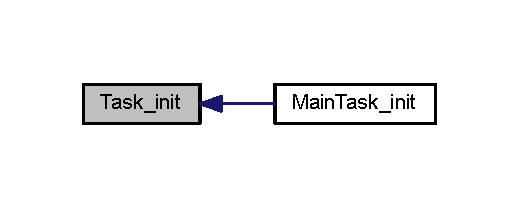
\includegraphics[width=249pt]{_task_8h_a4b074cf85d0db22ecd5abd511c33a2c4_icgraph}
\end{center}
\end{figure}



%--- End generated contents ---

% Index
\newpage
\phantomsection
\addcontentsline{toc}{chapter}{Index}
\printindex

\end{document}
